\documentclass[11pt,twoside]{book}
%Versión 4.0
% paquetes-----------------------------------------------------------------------------------------
\usepackage{lipsum} % para pruebas
\usepackage{pdftexcmds} %Para switch case
\usepackage[
paperwidth = 8.5in,
paperheight = 11in,
left = 1.25in,
right = 0.75in,
top = 0.950in,
bottom = 0.925in
]{geometry}
\usepackage{varwidth}
\usepackage{amsmath}
\usepackage{amsfonts}
\usepackage{amssymb}
\usepackage{graphicx}
\usepackage{pdfpages}
\usepackage{setspace} 
\usepackage{xltxtra}
\usepackage{enumitem}
\usepackage{xifthen}
\usepackage{xargs}
\usepackage{booktabs}
\usepackage{multirow}
\usepackage{pdflscape}
\usepackage{rotating}
\usepackage{bigstrut}
\usepackage{longtable}
\usepackage{fancyhdr}
\usepackage{url}
\usepackage{tocloft}
\usepackage[hidelinks, verbose]{hyperref}
\usepackage{colortbl}
\usepackage{multirow}
\usepackage{multicol}
\usepackage{changepage}
\usepackage[skins, breakable, hooks]{tcolorbox}
\usepackage[input-decimal-markers={.}, input-ignore={,}, group-separator={,}]{siunitx}
\usepackage{polyglossia}
\usepackage{tikz}
\usetikzlibrary{calc}
\usetikzlibrary{positioning}
\usepackage{array}
\usepackage{ragged2e} %Sirve para justificar texto
% \usepackage{fontspec} % se carga en xltxtra
% \usepackage{fixltx2e} % fixltx2e is not required with releases after 2015. All fixes are now in the LaTeX kernel.
% FIN-paquetes-------------------------------------------------------------------------------------
\setlength{\columnsep}{1.1cm} % estaba luego de multicol
\strictpagecheck % algo de changepage
\setmainlanguage{spanish} % de polyglossia
% leer pag 4 https://mirrors.ucr.ac.cr/CTAN/macros/latex/required/tools/array.pdf
% nuevos tipos de columnas
\newcolumntype{x}[1]{>{\centering\arraybackslash}p{#1}}
\newcolumntype{g}[1]{>{\raggedleft\arraybackslash}p{#1}}
\newcolumntype{q}[1]{>{\raggedright\arraybackslash}p{#1}}
% Tipo de letra
\usepackage[abspath]{currfile}
\setmainfont[
	Path=\currfileabsdir,
	BoldFont = Fuentes/OpenSans-CondBold.ttf ,
	ItalicFont = Fuentes/OpenSans-CondLightItalic.ttf ,
	BoldItalicFont = Fuentes/OpenSans-CondLightItalic.ttf
]{OpenSans-CondLight.ttf}
\newfontfamily\Bold{Open Sans Condensed Bold}
\newfontfamily\Sans{Open Sans}
\newfontfamily\SansBold{Open Sans Bold}
\newfontfamily\Italic{Open Sans Condensed Light Italic}
\newfontfamily\Logos{Latin Modern Roman}
\newfontfamily\Cinzel{Open Sans}
% diagramas de tikz
\tikzset{
    max width/.style args={#1}{
        execute at begin node={\begin{varwidth}{#1}},
        execute at end node={\end{varwidth}}
    }
}
\usetikzlibrary{shapes.geometric, arrows}
\tikzstyle{arrow} = [thick,->,>=stealth, to path={-| (\tikztotarget)}]
\tikzstyle{iniciofin} = [rectangle, minimum width=2cm, minimum height=0.7cm, text centered, draw=black, fill=blue!30, rounded corners]
\tikzstyle{process} = [rectangle, minimum width=3.5cm, minimum height=2cm, text centered, draw=black, max width=3.5cm]
\tikzstyle{decision} = [diamond, minimum width=3cm, minimum height=1cm, text centered, draw=black]
\tikzstyle{aux} = [fill=white,inner sep=0,outer sep=0]
\tikzstyle{diagrama} = [node distance=4cm, auto,scale=0.7, every node/.style={scale=0.7}]

% Estilo de página en blanco en el índice
\newcommand{\blank}{\addtocontents{toc}{\protect\thispagestyle{empty}}}

%título y fuente
\newcommand{\titulodoc}{Nombre del documento}
\newcommand{\lafuente}{Estadísticas INE}

\newcounter{Cuadro}[chapter]
\renewcommand{\theCuadro}{\thechapter.\arabic{Cuadro}}

\newcommand{\titulocuadro}[1]{\addtocounter{Cuadro}{1}
{\Bold\color{color1}{\normalsize Cuadro \theCuadro $\,-$  #1 }}
}

%%%%%%%%%%% Diseño global del documento
%	\setlength{\headsep}{0pt}
%	\setlength{\footskip}{46pt}
\setlength{\parindent}{1.5em}		%sangría
\setlength{\parskip}{2ex}		%separación entre párrafos  

%Distancias
\newlength{\cuadri} 
\setlength{\cuadri}{0.125in}

%Formato de contenidos
\setlength{\cftbeforetoctitleskip}{0em}
\AtBeginDocument{\addtocontents{toc}{\protect\thispagestyle{empty}}} 

\makeatletter
\renewcommand*\l@subsection{\@dottedtocline{2}{5.2em}{3.2em}}
\makeatother

\renewcommand{\thesection}{\thechapter.\arabic{section}}

\cftsetpnumwidth{2\cuadri}
\cftsetrmarg{8\cuadri}
\renewcommand{\cftsecnumwidth}{2.5\cuadri}
\renewcommand{\cftchapnumwidth}{2\cuadri}
\renewcommand{\cftsecindent}{2\cuadri}

%Colores base del documento
\definecolor{color1}{rgb}{0,0,0} % -Negro
%\definecolor{color2}{rgb}{0.56,0.36,0.65} %Debe ir en porcentaje de rgb (i.e. decimal) - morado rosadón
\definecolor{color2}{rgb}{0.45,0.44,0.78} % - Lila
%\definecolor{color2}{rgb}{0.09,0.47,0.27} % - Verde feminista
\definecolor{color3}{rgb}{0.2,0.2,0.5} %Debe ir en porcentaje de rgb (i.e. decimal) - Morado oscuro

%Para que las páginas en blanco no estén numeradas
\let\origdoublepage\cleardoublepage
\newcommand{\clearemptydoublepage}{
\clearpage
{\pagestyle{empty}\origdoublepage}
}
\let\cleardoublepage\clearemptydoublepage

%%%%%%%% Llamadas y notas al pie
\makeatletter
\newcommand{\markerspace}{\@ifnextchar.
{$\!$}{\@ifnextchar,
    {$\!$}{\@ifnextchar;
        {$\!$}{\@ifnextchar:
            {$\!$}{$\ $}
        }
    }
}}
\makeatother

\newcounter{numllamada}
\newcounter{numtextollamada}
\setcounter{numllamada}{0}
\setcounter{numtextollamada}{0}

\newcommand{\llamada}[1][\thenumllamada]{
	\stepcounter{numllamada}
	\begingroup
	\setcounter{mpfootnote}{#1}
	\renewcommand\thefootnote\thempfootnote$\hspace{0.2ex}$\footnotemark
	\endgroup
	\markerspace
}

\newcommand{\notita}[2][\thenumtextollamada]{
\stepcounter{numtextollamada}
\stepcounter{numllamada}
$\hspace{0.2ex}$
\footnote[#1]{#2}
}

\newcommand{\textollamada}[2][\thenumtextollamada]{
\ifthenelse{\equal{#1}{*}}
{
\begingroup
\renewcommand\thefootnote\thempfootnote\footnotetext[0]{#2\\[-1.7ex]}
\endgroup
}{
\stepcounter{numtextollamada}
\begingroup
\renewcommand\thefootnote\thempfootnote\footnotetext[#1]{#2}
\endgroup
}}

%redefinición de footnote
\newlength{\footnoterulewidth}
\setlength{\footnoterulewidth}{2.5cm}
\newlength{\footnoteruleheight}
\setlength{\footnoteruleheight}{.4pt} 
\makeatletter
\renewcommand{\footnoterule}{
	\kern -3pt
	\color{color2}
	\hrule width 
	\footnoterulewidth height 
	\footnoteruleheight
	\kern
	\dimexpr 3pt - \footnoteruleheight \relax
} 
\makeatother

\makeatletter
\renewcommand\@makefntext[1]{
	\noindent
	\makebox[1em][r]{\scriptsize\@makefnmark}
	\scriptsize#1
}
\makeatother

%%%%%%%%%%% tablas
\LTcapwidth=1.234\textwidth
\setlength{\arrayrulewidth}{0.8pt}
\arrayrulecolor{color2}

% Definición del comando cajita

\newtcolorbox{cajita-arriba}{
	width = 52\cuadri,
	height = 35\cuadri,
	enlarge left by = 0pt,
	enlarge top by = 1\cuadri,
	enlarge bottom by = 2\cuadri,
	nobeforeafter,
	opacityback=0, % Pone fondo transparente
	opacityframe=0, % Pone fondo transparente
	colframe=black, % Pone fondo transparente
%	colframe = white, % obsoleto, se dejó para referencia
%	colback = white, % obsoleto, se dejó para referencia
	left = -3pt,
	right = 0pt,
	bottom = 0pt,
	top = -3pt,
	arc = 0pt,
	boxrule = 0pt
}

\newtcolorbox{cajita-abajo}{
	width = 52\cuadri,
	height = 35\cuadri,
	enlarge top by = 0pt,
	enlarge left by = 0pt,
	enlarge bottom by = -2\cuadri,
	nobeforeafter,
	opacityback=0, % Pone fondo transparente
	opacityframe=0, % Pone fondo transparente
	colframe=black, % Pone fondo transparente
%	colframe = white, % obsoleto, se dejó para referencia
%	colback = white, % obsoleto, se dejó para referencia
	left = -3pt,
	right = 0pt,
	bottom = 0pt,
	top = -3pt,
	arc = 0pt,
	boxrule = 0pt
}

\newtcolorbox{cajota-unica}{
	width = 52\cuadri,
	height = 72\cuadri,
	enlarge left by = 0pt,
	enlarge top by  = 1\cuadri,
	enlarge bottom by = -2\cuadri,
	nobeforeafter,
	opacityback=0, % Pone fondo transparente
	opacityframe=0, % Pone fondo transparente
	colframe=black, % Pone fondo transparente
%	colframe = white, % obsoleto, se dejó para referencia
%	colback = white, % obsoleto, se dejó para referencia
	left = -3pt,
	right = 0pt,
	bottom =  0pt,
	top = -3pt,
	arc = 0pt,
	boxrule = 0pt
}

\newtcolorbox{descripcion-cajita}{
	width = 18\cuadri,
	height = 30.8\cuadri,
	nobeforeafter,
	opacityback=0, % Pone fondo transparente
	opacityframe=0, % Pone fondo transparente
	colframe=black, % Pone fondo transparente
	%colframe = white, % obsoleto, se dejó para referencia 
	%colback = white, % obsoleto, se dejó para referencia 
	left = -3pt,
	right = -3pt,
	bottom = -3pt,
	top = -8pt,
	arc = 0pt,
	boxrule = 0pt,
	enlarge bottom by = -29.78\cuadri
}

\newtcolorbox{grafica-cajita}{
	width = 32\cuadri,
	height = 30.8\cuadri,
	nobeforeafter,
	opacityback=0, % Pone fondo transparente
	opacityframe=0, % Pone fondo transparente
	colframe=black, % Pone fondo transparente
%	colframe = white, % obsoleto, se dejó para referencia
%	colback = white, % obsoleto, se dejó para referencia
	left = -3pt,
	right = -3pt,
	bottom = -3pt,
	top = -2pt,
	arc = 0pt,
	boxrule = 0pt,
	enlarge bottom by = -29.78\cuadri
}
% Cajas para fondos de capítulo y encabezado
\newtcolorbox{fondo-capitulo}{
	width = 8.5in,
	height = 11in,
	skin = enhancedmiddle, 
	nobeforeafter,
	watermark graphics = Plantilla/Capitulo_CEEG_2022.pdf,
	watermark opacity = 1.0,
	watermark overzoom = 1.0,
	enlarge left by=-1.475in,
	enlarge top by = -0.95in,
	enlarge bottom by = -20\cuadri,
	boxrule = 0pt,
	colframe = white,
	left = -3pt,
	bottom = -1pt,
	top = 8\cuadri,
	right = -3pt,
	arc = 0pt
}

% Cajas para agregar ODS



\newcommand{\cajitaODS}[1]{%
	\ifthenelse{ \equal{#1}{1} }{%
			\begin{tcolorbox}[
			width = 1.5cm,
	height = 1.5cm,
	skin = enhancedmiddle, 
	nobeforeafter,
	watermark graphics = Plantilla/ODS/ods1.pdf,
	watermark opacity = 1.0,
	watermark overzoom = 1.0,
	enlarge top by = 0.01in,
	enlarge bottom by = -1.5cm,
	boxrule = 0pt,
	colframe = white,
	colback = white,
	left = -3pt,
	bottom = -5in,
	top = -10\cuadri,
	right = -3pt,
	arc = 0pt]
\end{tcolorbox}	
	}%
	{}%
	\ifthenelse{\equal{#1}{2}}{%
			\begin{tcolorbox}[
			width = 1.5cm,
			height = 1.5cm,
			skin = enhancedmiddle, 
			nobeforeafter,
			watermark graphics = Plantilla/ODS/ods2.pdf,
			watermark opacity = 1.0,
			watermark overzoom = 1.0,
			enlarge top by = 0.01in,
			enlarge bottom by = -1.5cm,
			boxrule = 0pt,
			colframe = white,
			colback = white,
			left = -3pt,
			bottom = -5in,
			top = -10\cuadri,
			right = -3pt,
			arc = 0pt]
		\end{tcolorbox}	
	}%
	{}
		\ifthenelse{\equal{#1}{3}}{%
			\begin{tcolorbox}[
			width = 1.5cm,
	height = 1.5cm,
	skin = enhancedmiddle, 
	nobeforeafter,
	watermark graphics = Plantilla/ODS/ods3.pdf,
	watermark opacity = 1.0,
	watermark overzoom = 1.0,
	enlarge top by = 0.01in,
	enlarge bottom by = -1.5cm,
	boxrule = 0pt,
	colframe = white,
	colback = white,
	left = -3pt,
	bottom = -5in,
	top = -10\cuadri,
	right = -3pt,
	arc = 0pt]
\end{tcolorbox}	
	}%
	{}
		\ifthenelse{\equal{#1}{4}}{%
			\begin{tcolorbox}[
	width = 1.5cm,
	height = 1.5cm,
	skin = enhancedmiddle, 
	nobeforeafter,
	watermark graphics = Plantilla/ODS/ods4.pdf,
	watermark opacity = 1.0,
	watermark overzoom = 1.0,
	enlarge top by = 0.01in,
	enlarge bottom by = -1.5cm,
	boxrule = 0pt,
	colframe = white,
	colback = white,
	left = -3pt,
	bottom = -5in,
	top = -10\cuadri,
	right = -3pt,
	arc = 0pt]
\end{tcolorbox}	
	}%
	{}
		\ifthenelse{\equal{#1}{5}}{%
			\begin{tcolorbox}[
	width = 1.5cm,
	height = 1.5cm,
	skin = enhancedmiddle, 
	nobeforeafter,
	watermark graphics = Plantilla/ODS/ods5.pdf,
	watermark opacity = 1.0,
	watermark overzoom = 1.0,
	enlarge top by = 0.01in,
	enlarge bottom by = -1.5cm,
	boxrule = 0pt,
	colframe = white,
	colback = white,
	left = -3pt,
	bottom = -5in,
	top = -10\cuadri,
	right = -3pt,
	arc = 0pt]
\end{tcolorbox}	
	}%
	{}
		\ifthenelse{\equal{#1}{6}}{%
			\begin{tcolorbox}[
	width = 1.5cm,
	height = 1.5cm,
	skin = enhancedmiddle, 
	nobeforeafter,
	watermark graphics = Plantilla/ODS/ods6.pdf,
	watermark opacity = 1.0,
	watermark overzoom = 1.0,
	enlarge top by = 0.01in,
	enlarge bottom by = -1.5cm,
	boxrule = 0pt,
	colframe = white,
	colback = white,
	left = -3pt,
	bottom = -5in,
	top = -10\cuadri,
	right = -3pt,
	arc = 0pt]
\end{tcolorbox}	
	}%
	{}
		\ifthenelse{\equal{#1}{7}}{%
			\begin{tcolorbox}[
	width = 1.5cm,
	height = 1.5cm,
	skin = enhancedmiddle, 
	nobeforeafter,
	watermark graphics = Plantilla/ODS/ods7.pdf,
	watermark opacity = 1.0,
	watermark overzoom = 1.0,
	enlarge top by = 0.01in,
	enlarge bottom by = -1.5cm,
	boxrule = 0pt,
	colframe = white,
	colback = white,
	left = -3pt,
	bottom = -5in,
	top = -10\cuadri,
	right = -3pt,
	arc = 0pt]
\end{tcolorbox}	
	}%
	{}
		\ifthenelse{\equal{#1}{8}}{%
			\begin{tcolorbox}[
	width = 1.5cm,
	height = 1.5cm,
	skin = enhancedmiddle, 
	nobeforeafter,
	watermark graphics = Plantilla/ODS/ods8.pdf,
	watermark opacity = 1.0,
	watermark overzoom = 1.0,
	enlarge top by = 0.01in,
	enlarge bottom by = -1.5cm,
	boxrule = 0pt,
	colframe = white,
	colback = white,
	left = -3pt,
	bottom = -5in,
	top = -10\cuadri,
	right = -3pt,
	arc = 0pt]
\end{tcolorbox}	
	}%
	{}
	
			\ifthenelse{\equal{#1}{9}}{%
		\begin{tcolorbox}[
			width = 1.5cm,
			height = 1.5cm,
			skin = enhancedmiddle, 
			nobeforeafter,
			watermark graphics = Plantilla/ODS/ods9.pdf,
			watermark opacity = 1.0,
			watermark overzoom = 1.0,
			enlarge top by = 0.01in,
			enlarge bottom by = -1.5cm,
			boxrule = 0pt,
			colframe = white,
			colback = white,
			left = -3pt,
			bottom = -5in,
			top = -10\cuadri,
			right = -3pt,
			arc = 0pt]
		\end{tcolorbox}	
	}%
	{}
	
			\ifthenelse{\equal{#1}{10}}{%
		\begin{tcolorbox}[
			width = 1.5cm,
			height = 1.5cm,
			skin = enhancedmiddle, 
			nobeforeafter,
			watermark graphics = Plantilla/ODS/ods10.pdf,
			watermark opacity = 1.0,
			watermark overzoom = 1.0,
			enlarge top by = 0.01in,
			enlarge bottom by = -1.5cm,
			boxrule = 0pt,
			colframe = white,
			colback = white,
			left = -3pt,
			bottom = -5in,
			top = -10\cuadri,
			right = -3pt,
			arc = 0pt]
		\end{tcolorbox}	
	}%
	{}
	
			\ifthenelse{\equal{#1}{11}}{%
		\begin{tcolorbox}[
			width = 1.5cm,
			height = 1.5cm,
			skin = enhancedmiddle, 
			nobeforeafter,
			watermark graphics = Plantilla/ODS/ods11.pdf,
			watermark opacity = 1.0,
			watermark overzoom = 1.0,
			enlarge top by = 0.01in,
			enlarge bottom by = -1.5cm,
			boxrule = 0pt,
			colframe = white,
			colback = white,
			left = -3pt,
			bottom = -5in,
			top = -10\cuadri,
			right = -3pt,
			arc = 0pt]
		\end{tcolorbox}	
	}%
	{}
	
			\ifthenelse{\equal{#1}{12}}{%
		\begin{tcolorbox}[
			width = 1.5cm,
			height = 1.5cm,
			skin = enhancedmiddle, 
			nobeforeafter,
			watermark graphics = Plantilla/ODS/ods12.pdf,
			watermark opacity = 1.0,
			watermark overzoom = 1.0,
			enlarge top by = 0.01in,
			enlarge bottom by = -1.5cm,
			boxrule = 0pt,
			colframe = white,
			colback = white,
			left = -3pt,
			bottom = -5in,
			top = -10\cuadri,
			right = -3pt,
			arc = 0pt]
		\end{tcolorbox}	
	}%
	{}
	
			\ifthenelse{\equal{#1}{13}}{%
		\begin{tcolorbox}[
			width = 1.5cm,
			height = 1.5cm,
			skin = enhancedmiddle, 
			nobeforeafter,
			watermark graphics = Plantilla/ODS/ods13.pdf,
			watermark opacity = 1.0,
			watermark overzoom = 1.0,
			enlarge top by = 0.01in,
			enlarge bottom by = -1.5cm,
			boxrule = 0pt,
			colframe = white,
			colback = white,
			left = -3pt,
			bottom = -5in,
			top = -10\cuadri,
			right = -3pt,
			arc = 0pt]
		\end{tcolorbox}	
	}%
	{}
	
			\ifthenelse{\equal{#1}{14}}{%
		\begin{tcolorbox}[
			width = 1.5cm,
			height = 1.5cm,
			skin = enhancedmiddle, 
			nobeforeafter,
			watermark graphics = Plantilla/ODS/ods14.pdf,
			watermark opacity = 1.0,
			watermark overzoom = 1.0,
			enlarge top by = 0.01in,
			enlarge bottom by = -1.5cm,
			boxrule = 0pt,
			colframe = white,
			colback = white,
			left = -3pt,
			bottom = -5in,
			top = -10\cuadri,
			right = -3pt,
			arc = 0pt]
		\end{tcolorbox}	
	}%
	{}
	
			\ifthenelse{\equal{#1}{15}}{%
		\begin{tcolorbox}[
			width = 1.5cm,
			height = 1.5cm,
			skin = enhancedmiddle, 
			nobeforeafter,
			watermark graphics = Plantilla/ODS/ods15.pdf,
			watermark opacity = 1.0,
			watermark overzoom = 1.0,
			enlarge top by = 0.01in,
			enlarge bottom by = -1.5cm,
			boxrule = 0pt,
			colframe = white,
			colback = white,
			left = -3pt,
			bottom = -5in,
			top = -10\cuadri,
			right = -3pt,
			arc = 0pt]
		\end{tcolorbox}	
	}%
	{}
	
			\ifthenelse{\equal{#1}{16}}{%
		\begin{tcolorbox}[
			width = 1.5cm,
			height = 1.5cm,
			skin = enhancedmiddle, 
			nobeforeafter,
			watermark graphics = Plantilla/ODS/ods16.pdf,
			watermark opacity = 1.0,
			watermark overzoom = 1.0,
			enlarge top by = 0.01in,
			enlarge bottom by = -1.5cm,
			boxrule = 0pt,
			colframe = white,
			colback = white,
			left = -3pt,
			bottom = -5in,
			top = -10\cuadri,
			right = -3pt,
			arc = 0pt]
		\end{tcolorbox}	
	}%
	{}
	
			\ifthenelse{\equal{#1}{17}}{%
		\begin{tcolorbox}[
			width = 1.5cm,
			height = 1.5cm,
			skin = enhancedmiddle, 
			nobeforeafter,
			watermark graphics = Plantilla/ODS/ods17.pdf,
			watermark opacity = 1.0,
			watermark overzoom = 1.0,
			enlarge top by = 0.01in,
			enlarge bottom by = -1.5cm,
			boxrule = 0pt,
			colframe = white,
			colback = white,
			left = -3pt,
			bottom = -5in,
			top = -10\cuadri,
			right = -3pt,
			arc = 0pt]
		\end{tcolorbox}	
	}%
	{}
	
}

\newcommand{\cajitaODSArriba}[1]{%
				\ifthenelse{\equal{#1}{1}}{%
				\begin{tcolorbox}[
			width = 1.5cm,
			height = 1.5cm,
			skin = enhancedmiddle, 
			nobeforeafter,
			watermark graphics = Plantilla/ODS/ods1.pdf,
			watermark opacity = 1.0,
			watermark overzoom = 1.0,
			enlarge top by = -5mm,
			enlarge bottom by = -1cm,
			boxrule = 0pt,
			colframe = white,
			colback = white,
			arc = 0pt]
		\end{tcolorbox}	
	}%
	{}
	
					\ifthenelse{\equal{#1}{2}}{%
		\begin{tcolorbox}[
			width = 1.5cm,
			height = 1.5cm,
			skin = enhancedmiddle, 
			nobeforeafter,
			watermark graphics = Plantilla/ODS/ods2.pdf,
			watermark opacity = 1.0,
			watermark overzoom = 1.0,
			enlarge top by = -5mm,
			enlarge bottom by = -1cm,
			boxrule = 0pt,
			colframe = white,
			colback = white,
			arc = 0pt]
		\end{tcolorbox}	
	}%
	{}
					\ifthenelse{\equal{#1}{3}}{%
		\begin{tcolorbox}[
			width = 1.5cm,
			height = 1.5cm,
			skin = enhancedmiddle, 
			nobeforeafter,
			watermark graphics = Plantilla/ODS/ods3.pdf,
			watermark opacity = 1.0,
			watermark overzoom = 1.0,
			enlarge top by = -5mm,
			enlarge bottom by = -1cm,
			boxrule = 0pt,
			colframe = white,
			colback = white,
			arc = 0pt]
		\end{tcolorbox}	
	}%
	{}
	
					\ifthenelse{\equal{#1}{4}}{%
		\begin{tcolorbox}[
			width = 1.5cm,
			height = 1.5cm,
			skin = enhancedmiddle, 
			nobeforeafter,
			watermark graphics = Plantilla/ODS/ods4.pdf,
			watermark opacity = 1.0,
			watermark overzoom = 1.0,
			enlarge top by = -5mm,
			enlarge bottom by = -1cm,
			boxrule = 0pt,
			colframe = white,
			colback = white,
			arc = 0pt]
		\end{tcolorbox}	
	}%
	{}
	
					\ifthenelse{\equal{#1}{5}}{%
		\begin{tcolorbox}[
			width = 1.5cm,
			height = 1.5cm,
			skin = enhancedmiddle, 
			nobeforeafter,
			watermark graphics = Plantilla/ODS/ods5.pdf,
			watermark opacity = 1.0,
			watermark overzoom = 1.0,
			enlarge top by = -5mm,
			enlarge bottom by = -1cm,
			boxrule = 0pt,
			colframe = white,
			colback = white,
			arc = 0pt]
		\end{tcolorbox}	
	}%
	{}
	
					\ifthenelse{\equal{#1}{6}}{%
		\begin{tcolorbox}[
			width = 1.5cm,
			height = 1.5cm,
			skin = enhancedmiddle, 
			nobeforeafter,
			watermark graphics = Plantilla/ODS/ods6.pdf,
			watermark opacity = 1.0,
			watermark overzoom = 1.0,
			enlarge top by = -5mm,
			enlarge bottom by = -1cm,
			boxrule = 0pt,
			colframe = white,
			colback = white,
			arc = 0pt]
		\end{tcolorbox}	
	}%
	{}
	
					\ifthenelse{\equal{#1}{7}}{%
		\begin{tcolorbox}[
			width = 1.5cm,
			height = 1.5cm,
			skin = enhancedmiddle, 
			nobeforeafter,
			watermark graphics = Plantilla/ODS/ods7.pdf,
			watermark opacity = 1.0,
			watermark overzoom = 1.0,
			enlarge top by = -5mm,
			enlarge bottom by = -1cm,
			boxrule = 0pt,
			colframe = white,
			colback = white,
			arc = 0pt]
		\end{tcolorbox}	
	}%
	{}
	
					\ifthenelse{\equal{#1}{8}}{%
		\begin{tcolorbox}[
			width = 1.5cm,
			height = 1.5cm,
			skin = enhancedmiddle, 
			nobeforeafter,
			watermark graphics = Plantilla/ODS/ods8.pdf,
			watermark opacity = 1.0,
			watermark overzoom = 1.0,
			enlarge top by = -5mm,
			enlarge bottom by = -1cm,
			boxrule = 0pt,
			colframe = white,
			colback = white,
			arc = 0pt]
		\end{tcolorbox}	
	}%
	{}
	
					\ifthenelse{\equal{#1}{9}}{%
		\begin{tcolorbox}[
			width = 1.5cm,
			height = 1.5cm,
			skin = enhancedmiddle, 
			nobeforeafter,
			watermark graphics = Plantilla/ODS/ods9.pdf,
			watermark opacity = 1.0,
			watermark overzoom = 1.0,
			enlarge top by = -5mm,
			enlarge bottom by = -1cm,
			boxrule = 0pt,
			colframe = white,
			colback = white,
			arc = 0pt]
		\end{tcolorbox}	
	}%
	{}
	
					\ifthenelse{\equal{#1}{10}}{%
		\begin{tcolorbox}[
			width = 1.5cm,
			height = 1.5cm,
			skin = enhancedmiddle, 
			nobeforeafter,
			watermark graphics = Plantilla/ODS/ods10.pdf,
			watermark opacity = 1.0,
			watermark overzoom = 1.0,
			enlarge top by = -5mm,
			enlarge bottom by = -1cm,
			boxrule = 0pt,
			colframe = white,
			colback = white,
			arc = 0pt]
		\end{tcolorbox}	
	}%
	{}
	
					\ifthenelse{\equal{#1}{11}}{%
		\begin{tcolorbox}[
			width = 1.5cm,
			height = 1.5cm,
			skin = enhancedmiddle, 
			nobeforeafter,
			watermark graphics = Plantilla/ODS/ods11.pdf,
			watermark opacity = 1.0,
			watermark overzoom = 1.0,
			enlarge top by = -5mm,
			enlarge bottom by = -1cm,
			boxrule = 0pt,
			colframe = white,
			colback = white,
			arc = 0pt]
		\end{tcolorbox}	
	}%
	{}
	
					\ifthenelse{\equal{#1}{12}}{%
		\begin{tcolorbox}[
			width = 1.5cm,
			height = 1.5cm,
			skin = enhancedmiddle, 
			nobeforeafter,
			watermark graphics = Plantilla/ODS/ods12.pdf,
			watermark opacity = 1.0,
			watermark overzoom = 1.0,
			enlarge top by = -5mm,
			enlarge bottom by = -1cm,
			boxrule = 0pt,
			colframe = white,
			colback = white,
			arc = 0pt]
		\end{tcolorbox}	
	}%
	{}
	
					\ifthenelse{\equal{#1}{13}}{%
		\begin{tcolorbox}[
			width = 1.5cm,
			height = 1.5cm,
			skin = enhancedmiddle, 
			nobeforeafter,
			watermark graphics = Plantilla/ODS/ods13.pdf,
			watermark opacity = 1.0,
			watermark overzoom = 1.0,
			enlarge top by = -5mm,
			enlarge bottom by = -1cm,
			boxrule = 0pt,
			colframe = white,
			colback = white,
			arc = 0pt]
		\end{tcolorbox}	
	}%
	{}
	
					\ifthenelse{\equal{#1}{14}}{%
		\begin{tcolorbox}[
			width = 1.5cm,
			height = 1.5cm,
			skin = enhancedmiddle, 
			nobeforeafter,
			watermark graphics = Plantilla/ODS/ods14.pdf,
			watermark opacity = 1.0,
			watermark overzoom = 1.0,
			enlarge top by = -5mm,
			enlarge bottom by = -1cm,
			boxrule = 0pt,
			colframe = white,
			colback = white,
			arc = 0pt]
		\end{tcolorbox}	
	}%
	{}
	
					\ifthenelse{\equal{#1}{15}}{%
		\begin{tcolorbox}[
			width = 1.5cm,
			height = 1.5cm,
			skin = enhancedmiddle, 
			nobeforeafter,
			watermark graphics = Plantilla/ODS/ods15.pdf,
			watermark opacity = 1.0,
			watermark overzoom = 1.0,
			enlarge top by = -5mm,
			enlarge bottom by = -1cm,
			boxrule = 0pt,
			colframe = white,
			colback = white,
			arc = 0pt]
		\end{tcolorbox}	
	}%
	{}
	
					\ifthenelse{\equal{#1}{16}}{%
		\begin{tcolorbox}[
			width = 1.5cm,
			height = 1.5cm,
			skin = enhancedmiddle, 
			nobeforeafter,
			watermark graphics = Plantilla/ODS/ods16.pdf,
			watermark opacity = 1.0,
			watermark overzoom = 1.0,
			enlarge top by = -5mm,
			enlarge bottom by = -1cm,
			boxrule = 0pt,
			colframe = white,
			colback = white,
			arc = 0pt]
		\end{tcolorbox}	
	}%
	{}
	
					\ifthenelse{\equal{#1}{17}}{%
		\begin{tcolorbox}[
			width = 1.5cm,
			height = 1.5cm,
			skin = enhancedmiddle, 
			nobeforeafter,
			watermark graphics = Plantilla/ODS/ods17.pdf,
			watermark opacity = 1.0,
			watermark overzoom = 1.0,
			enlarge top by = -5mm,
			enlarge bottom by = -1cm,
			boxrule = 0pt,
			colframe = white,
			colback = white,
			arc = 0pt]
		\end{tcolorbox}	
	}%
	{}


}


\newtcolorbox{parte-toc}{
	width = 52\cuadri,
	enlarge left by = 0pt,
	enlarge top by = 0\cuadri,
	enlarge bottom by = 0\cuadri,
	nobeforeafter,
	colframe = color1!90!black,
	colback = white,
	left = 3pt,
	right = 0pt,
	bottom = 0pt,
	top = 0pt,
	arc = 0pt,
	boxrule = 0pt,
	leftrule = 4pt
}

\newtcolorbox{fondo-parte}{
	width=8.5in,
	height=11in,
	skin=enhancedmiddle,
	nobeforeafter,
	watermark graphics=Plantilla/parte.pdf,
	watermark opacity=1.0,
	watermark overzoom=1.0,
	enlarge left by=-1.455in,
	enlarge top by=-0.95in, 
	enlarge bottom by=-20\cuadri,
	boxrule=0pt,
	colframe=white,
	left=-3pt,
	bottom=-1pt,
	top=8\cuadri,
	right=-3pt,
	arc=0pt
}

\newtcolorbox{fondo-capitulo-no-descripcion}{
	width=8.5in,
	height=11in,
	skin=enhancedmiddle,
	nobeforeafter,
	watermark graphics=Plantilla/Apendice_CEEG_2022.pdf,
	watermark opacity=1.0,
	watermark overzoom=1.0,
	enlarge left by=-1.475in,
	enlarge top by=-0.95in,
	enlarge bottom by=-20\cuadri,
	boxrule=0pt,
	colframe=white,
	left=-3pt,
	bottom=-1pt,
	top=8\cuadri,
	right=-3pt,
	arc=0pt
}

\newtcolorbox{numcapitulo}{
	height=1.2in,
	width=1.12in,
	enlarge top by= -1.3in,
	enlarge bottom by=-0.47in,
	boxrule=3pt,arc=3pt,
	colframe=white,
	colback=white,
	right=2pt,
	left=3pt,
	top=14pt,
	bottom=2pt
}

\newtcolorbox{encabezadoimpar}{
	width=8.5in,
	height=11.01in,
	skin=enhancedmiddle,
	nobeforeafter,
	watermark graphics=Plantilla/Cintillo_Derecha_CEEG_2022.pdf,
%	watermark opacity=1.0,
	watermark overzoom=1.0,
	enlarge left by=-1.25in,
	enlarge top by=-0.51in,
	enlarge bottom by=3\cuadri,
	boxrule=0pt, colframe=white,
	left=0.71in,
	bottom=-1pt,
	top=2.5\cuadri,
	right=0.71in,
	arc=0pt
}

\newtcolorbox{encabezadopar}{
	width=8.5in,
	height=11.01in,
	skin=enhancedmiddle,
	nobeforeafter,
	watermark graphics=Plantilla/Cintillo_Izquierda_CEEG_2022.pdf,
	watermark opacity=1.0,
	watermark overzoom=1.0,
	enlarge left by=-0.75in,
	enlarge top by=-0.51in,
	enlarge bottom by=3\cuadri,
	boxrule=0pt,
	colframe=white,
	left=0.71in,
	bottom=-1pt,
	top=2.5\cuadri,
	right=0.71in,
	arc=0pt
}

\newtcbox{numpag}{
	colback=color1,
	colframe=color1,
	arc=0pt,
	top=3pt,
	bottom=2pt,
	left=3pt,
	right=3pt,
	nobeforeafter,
	enlarge top by=-0.125in
}

%%%%%%%%%%% Encabezado y pie de página
\fancypagestyle{estandar}{
	\fancyhf{}
	\renewcommand{\headrulewidth}{0pt}
	\fancyhead[CO]{
		\begin{encabezadoimpar}
		\end{encabezadoimpar}
	}
	\fancyfoot[RO]{
		\color{color3}{\capituloencabezado \ \ }
		\color{color3}
		\raisebox{0.5mm}{$\mid$}
		\color{color3}
		\textbf{ \ \ \ \thepage}
	}
	\fancyhead[CE]{
		\begin{encabezadopar}
		\end{encabezadopar}
	}
	\fancyhead[CO]{
		\begin{encabezadoimpar}
		\end{encabezadoimpar}
	}
	\fancyfoot[LE]{
		\color{color3}
		\textbf{\thepage \ \ \ }
		\color{black}
		\raisebox{0.5mm}{$\mid$}
		\color{color3}{ \ \  \titulodoc}
	}
}

\fancypagestyle{soloarriba}{
	\fancyhf{}
	\renewcommand{\headrulewidth}{0pt}
	\fancyhead[CO]{
		\begin{encabezadoimpar}
		\end{encabezadoimpar}
	}
	\fancyfoot[RO]{}
	\fancyhead[CE]{
		\begin{encabezadopar}
		\end{encabezadopar}
	}
	\fancyfoot[LE]{}
}

\pagestyle{estandar}

%%%%%%%%%%% Macros de cajitas
%  El comando se escribe así: \cajita[Sección en índice]{Sección en cuerpo}{Descripción}{Título gráfica}{Desagregación}{Gráfica con \includegraphics o tikz}{Fuente}
\newcounter{updown}
\setcounter{updown}{0}

\newcommand{\cajitaalternante}[1]{
\ifthenelse{\equal{\theupdown}{0}}{
	\noindent
	\begin{cajita-arriba}
		\phantomsection
		\stepcounter{section} #1
	\end{cajita-arriba}
	\setcounter{updown}{1}
	}{
	\noindent
	\begin{cajita-abajo}
		\phantomsection
		\stepcounter{section} #1
	\end{cajita-abajo}
	\setcounter{updown}{0}
	}
}

\newcommand{\titulizador}[1]{
	\begin{tabular}{@{}p{3.5\cuadri}p{3pt}@{}p{46.0\cuadri}}
		& &\\[-1\cuadri]
		\textbf{\color{color3}\huge \thesection}$\ $ & & \textbf{\color{color3}\huge #1}\\[-1\cuadri]
	\end{tabular}
}

\newcommand{\titulizadormanual}[2]{
	\begin{tabular}{@{}p{3.5\cuadri}|p{3pt}@{}p{46.0\cuadri}}
		& &\\[-1\cuadri]
		\textbf{\color{color2}\Large #2}$\ $ & &\textbf{\Large #1}\\[-1\cuadri]
		& &\\[-0.8pt] \cline{2-3}
	\end{tabular}
}

\newcommand{\cajitaderecha}[8][]{%
	\ifthenelse{\isempty{#1}}{
		\cajitaalternante{
			\addcontentsline{toc}{section}{\numberline{\thesection} #2}
			\addtocontents{toc}{\protect\thispagestyle{empty}}
			\titulizador{#2}
			\begin{tabular}[b]{@{}p{17.5\cuadri}@{}p{1.5\cuadri}@{} x{34\cuadri}@{}x{3\cuadri}}
				 &  &  &  \\[\cuadri]
				\begin{descripcion-cajita}
					\parskip 6pt\parindent 1em 
					#3
				\end{descripcion-cajita}
				&  &
				\begin{grafica-cajita}
				\begin{center}
					\ifthenelse{\isempty{#4}}{}{{\textbf{\color{color2}#4}}\\[-1pt]}
					\ifthenelse{\isempty{#5}}{
						$\ $\\[-0.1\cuadri]
					}{
						{\footnotesize\texttwelveudash$\,\,$#5$\,\,$\texttwelveudash}\\[0.6\cuadri]
					}
					#6
					\begin{flushleft}
						$\ $\\[-2\cuadri]
						\ \ \ \footnotesize Fuente: #7
					\end{flushleft}
				\end{center}
			
				\end{grafica-cajita}& \ifthenelse{\isempty{#8}}{}{\cajitaODS{#8} }
			\end{tabular}
		}
	}{
		\cajitaalternante{
			\addcontentsline{toc}{section}{\numberline{\thesection} #1}
			\addtocontents{toc}{\protect\thispagestyle{empty}}
			\titulizador{#2}

			\begin{tabular}[b]{@{}p{17.5\cuadri}@{}p{1.5\cuadri}@{} x{34\cuadri}@{}x{3\cuadri}}
				 &  &  & \\[\cuadri]
				\begin{descripcion-cajita}
					\parskip 6pt\parindent 1em%
					#3
				\end{descripcion-cajita}
				&  &
				\begin{grafica-cajita}
					\begin{center}
						\ifthenelse{\isempty{#4}}{}{{\textbf{\color{color2}#4}}\\[-1pt]}%
						\ifthenelse{\isempty{#5}}{
							$\ $\\[-0.1\cuadri]
						}{
							{\footnotesize\texttwelveudash$\,\,$#5$\,\,$\texttwelveudash}\\[0.6\cuadri]
						}
						#6
						\begin{flushleft}
							$\ $\\[-2\cuadri]
							\ \ \ \footnotesize Fuente: #7
						\end{flushleft}
					\end{center}
				\end{grafica-cajita} & & \ifthenelse{\isempty{#8}}{}{\cajitaODS{#8} }
			\end{tabular}
		}
	}
}

\newcommand{\cajitaizquierda}[8][]{
	\ifthenelse{\isempty{#1}}{
		\cajitaalternante{
			\addcontentsline{toc}{section}{\numberline{\thesection} #2}
			\addtocontents{toc}{\protect\thispagestyle{empty}}
			\titulizador{#2}
			\begin{tabular}[b]{@{}p{34\cuadri}@{}p{0\cuadri}@{} x{17.5\cuadri}@{}x{7\cuadri}}
				&  &  &  \\[\cuadri]
				\begin{grafica-cajita}
					\begin{center}
						\ifthenelse{\isempty{#4}}{}{{\textbf{\color{color2}#4}}\\[-1pt]}%
						\ifthenelse{\isempty{#5}}{
							$\ $\\[-0.1\cuadri]
						}{
							{\footnotesize\texttwelveudash$\,\,$#5$\,\,$\texttwelveudash}\\[0.6\cuadri]
						}
						#6
						\begin{flushleft}
							$\ $\\[-2\cuadri]
							\ \ \ \footnotesize Fuente: #7
						\end{flushleft}
					\end{center}
				\end{grafica-cajita}
				& &
				\begin{descripcion-cajita}
					\parskip 6pt\parindent 1em%
					#3
				\end{descripcion-cajita} & \ifthenelse{\isempty{#8}}{}{\cajitaODSArriba{#8} }
			\end{tabular}
		}
	}{
		\cajitaalternante{
			\addcontentsline{toc}{section}{\numberline{\thesection} #1}
			\addtocontents{toc}{\protect\thispagestyle{empty}}
			\titulizador{#2}
			\begin{tabular}[b]{@{}p{34\cuadri}@{}p{0\cuadri}@{} x{17.5\cuadri}@{}x{7\cuadri}}
				&  &  & \\[0.5\cuadri]
				\begin{grafica-cajita}
					\begin{center}
						\ifthenelse{\isempty{#4}}{}{{\textbf{\color{color2}#4}}\\[-1pt]}%
						\ifthenelse{\isempty{#5}}{
							$\ $\\[-0.1\cuadri]
						}{
							{\footnotesize\texttwelveudash$\,\,$#5$\,\,$\texttwelveudash}\\[0.6\cuadri]
						}
						#6
						\begin{flushleft}
							$\ $\\[-2\cuadri]
							\ \ \ \footnotesize Fuente: #7
						\end{flushleft}
					\end{center}
				\end{grafica-cajita}
				& &
				\begin{descripcion-cajita}
					\parskip 6pt\parindent 1em%
					#3
				\end{descripcion-cajita}& \ifthenelse{\isempty{#8}}{}{\cajitaODSArriba{#8} }
			\end{tabular}
		}
	}
}

\newcommand{\cajita}[8][]{
	\ifthenelse{\equal{\theupdown}{0}}{
		\cajitaizquierda[#1]{#2}{#3}{#4}{#5}{#6}{#7}{#8}
	}{
		\cajitaderecha[#1]{#2}{#3}{#4}{#5}{#6}{#7}{#8}
	}
}
%%%%%%%%%%%%%%%  Cajita manual
\newcommand{\cajitaderechamanual}[8][]{
	\ifthenelse{\isempty{#1}}{
		\cajitaalternante{
			\addcontentsline{toc}{section}{\numberline{\thesection} #2}
			\addtocontents{toc}{\protect\thispagestyle{empty}}
			\titulizadormanual{#2}{#8}
			\begin{tabular}[b]{@{}p{17.5\cuadri}@{}p{1.5\cuadri}@{} x{34\cuadri}@{}}
				& &\\[0.5\cuadri]
				\begin{descripcion-cajita}
				\parskip 6pt\parindent 1em
				#3
				\end{descripcion-cajita}
				& &
				\begin{grafica-cajita}
					\begin{center}
						\ifthenelse{\isempty{#4}}{}{{\textbf{\color{color2}#4}}\\[-1pt]}
						\ifthenelse{\isempty{#5}}{
							$\ $\\[-0.1\cuadri]
						}{
							{\footnotesize\texttwelveudash$\,\,$#5$\,\,$\texttwelveudash}\\[0.6\cuadri]
						}
						#6
						\begin{flushleft}
							$\ $\\[-2\cuadri]
							\ \ \ \footnotesize Fuente: #7
						\end{flushleft}
					\end{center}
				\end{grafica-cajita}
			\end{tabular}
		}
	}{
		\cajitaalternante{
			\addcontentsline{toc}{section}{\numberline{\thesection} #1}
			\addtocontents{toc}{\protect\thispagestyle{empty}}
			\titulizadormanual{#2}{#8}
			\begin{tabular}[b]{@{}p{17.5\cuadri}@{}p{1.5\cuadri}@{} x{34\cuadri}@{}}
				& &\\[0.5\cuadri]
				\begin{descripcion-cajita}
					\parskip 6pt\parindent 1em
					#3
					\end{descripcion-cajita}
					& &
				\begin{grafica-cajita}
					\begin{center}
						\ifthenelse{\isempty{#4}}{}{{\textbf{\color{color2}#4}}\\[-1pt]}%
						\ifthenelse{\isempty{#5}}{
							$\ $\\[-0.1\cuadri]
						}{
							{\footnotesize\texttwelveudash$\,\,$#5$\,\,$\texttwelveudash}\\[0.6\cuadri]
						}
						#6
						\begin{flushleft}
							$\ $\\[-2\cuadri]
							\ \ \ \footnotesize Fuente: #7
						\end{flushleft}
					\end{center}
				\end{grafica-cajita}
			\end{tabular}
		}
	}
}

\newcommand{\cajitaizquierdamanual}[8][]{
	\ifthenelse{\isempty{#1}}{
		\cajitaalternante{
			\addcontentsline{toc}{section}{\numberline{\thesection} #2}
			\addtocontents{toc}{\protect\thispagestyle{empty}}
			\titulizadormanual{#2}{#8}
			\begin{tabular}[b]{@{}p{34\cuadri}@{}p{0\cuadri}@{} x{17.5\cuadri}@{}}
				& &\\[0.5\cuadri]
				\begin{grafica-cajita}
					\begin{center}
						\ifthenelse{\isempty{#4}}{}{{\textbf{\color{color2}#4}}\\[-1pt]}
						\ifthenelse{\isempty{#5}}{
							$\ $\\[-0.1\cuadri]
						}{
							{\footnotesize\texttwelveudash$\,\,$#5$\,\,$\texttwelveudash}\\[0.6\cuadri]
						}
						#6
						\begin{flushleft}
							$\ $\\[-2\cuadri]
							\ \ \ \footnotesize Fuente: #7
						\end{flushleft}
					\end{center}
				\end{grafica-cajita}
				& &
				\begin{descripcion-cajita}
					\parskip 6pt\parindent 1em
					#3
				\end{descripcion-cajita}
			\end{tabular}
		}
	}{
	\cajitaalternante{
		\addcontentsline{toc}{section}{\numberline{\thesection} #1}
		\addtocontents{toc}{\protect\thispagestyle{empty}}
		\titulizadormanual{#2}{#8}
		\begin{tabular}[b]{@{}p{34\cuadri}@{}p{0\cuadri}@{} x{17.5\cuadri}@{}}
			& &\\[0.5\cuadri]
			\begin{grafica-cajita}
				\begin{center}
					\ifthenelse{\isempty{#4}}{}{{\textbf{\color{color2}#4}}\\[-1pt]}
					\ifthenelse{\isempty{#5}}{
						$\ $\\[-0.1\cuadri]
					}{
						{\footnotesize\texttwelveudash$\,\,$#5$\,\,$\texttwelveudash}\\[0.6\cuadri]
					}
					#6
					\begin{flushleft}
						$\ $\\[-2\cuadri]
						\ \ \ \footnotesize Fuente: #7
					\end{flushleft}
				\end{center}
			\end{grafica-cajita}
			& &
			\begin{descripcion-cajita}
				\parskip 6pt\parindent 1em
				#3
			\end{descripcion-cajita}
		\end{tabular}
		}
	}
}

\newcommand{\cajitamanual}[8][]{
	\ifthenelse{\equal{\theupdown}{0}}{
		\cajitaizquierdamanual[#1]{#2}{#3}{#4}{#5}{#6}{#7}{#8}
	}{
		\cajitaderechamanual[#1]{#2}{#3}{#4}{#5}{#6}{#7}{#8}
	}
}

%%%%%%%%%%%%%%%  Cajita de tabla
\newcommand{\cajitaizquierdatabla}[7][]{
	\ifthenelse{\isempty{#1}}{
		\cajitaalternante{
			\addcontentsline{toc}{section}{\numberline{\thesection} #2}
			\addtocontents{toc}{\protect\thispagestyle{empty}}
			\titulizador{#2}
			\begin{tabular}[b]{@{}p{34\cuadri}@{}p{0\cuadri}@{} x{17.5\cuadri}@{}}
				& &\\[0.5\cuadri]
				\begin{grafica-cajita}
					\begin{center}
						\ifthenelse{\isempty{#4}}{}{{\textbf{\color{color2}#4}}\\[-1pt]}
						\ifthenelse{\isempty{#5}}{$\ $\\[-0.1\cuadri]}{
							{\footnotesize\texttwelveudash$\,\,$#5$\,\,$\texttwelveudash}\\[0.6\cuadri]}
						\ifthenelse{\isempty{#7}}{\renewcommand{\lafuente}{Estadísticas INE}}{\renewcommand{\lafuente}{#7}}
						\begin{tabular}{l}
							#6\\[4mm]
							$\ $\\[-3.5mm]
							{\footnotesize $\ \ \ $Fuente: \lafuente}
						\end{tabular}
					\end{center}
				\end{grafica-cajita}
				& &
				\begin{descripcion-cajita}
					\parskip 6pt\parindent 1em
					#3
				\end{descripcion-cajita}
			\end{tabular}
		}
	}{
		\cajitaalternante{
			\addcontentsline{toc}{section}{\numberline{\thesection} #1}
			\addtocontents{toc}{\protect\thispagestyle{empty}}
			\titulizador{#2}
			\begin{tabular}[b]{@{}p{34\cuadri}@{}p{0\cuadri}@{} x{17.5\cuadri}@{}}
				& &\\[0.5\cuadri]
				\begin{grafica-cajita}
					\begin{center}
						\ifthenelse{\isempty{#4}}{}{{\textbf{\color{color2}#4}}\\[-1pt]}
						\ifthenelse{\isempty{#5}}{
							$\ $\\[-0.1\cuadri]
						}{
							{\footnotesize\texttwelveudash$\,\,$#5$\,\,$\texttwelveudash}\\[0.6\cuadri]
						}
						\ifthenelse{\isempty{#7}}{
							\renewcommand{\lafuente}{Estadísticas INE}
						}{
							\renewcommand{\lafuente}{#7}
						}
						\begin{tabular}{l}
							#6\\[4mm]
							$\ $\\[-3.5mm]
							{\footnotesize $\ \ \ $Fuente: \lafuente}
						\end{tabular}
					\end{center}
				\end{grafica-cajita}
				& &
				\begin{descripcion-cajita}
					\parskip 6pt\parindent 1em
					#3
				\end{descripcion-cajita}
			\end{tabular}
		}
	}
}

\newcommand{\cajitaderechatabla}[7][]{
	\ifthenelse{\isempty{#1}}{
		\cajitaalternante{
			\addcontentsline{toc}{section}{\numberline{\thesection} #2}
			\addtocontents{toc}{\protect\thispagestyle{empty}}
			\titulizador{#2}
			\begin{tabular}[b]{@{}p{17.5\cuadri}@{}p{1.5\cuadri}@{} x{34\cuadri}@{}}
				& &\\[0.5\cuadri]
				\begin{descripcion-cajita}
					\parskip 6pt\parindent 1em
					#3
				\end{descripcion-cajita}
				& &
				\begin{grafica-cajita}
					\begin{center}
						\ifthenelse{\isempty{#4}}{}{{\textbf{\color{color2}#4}}\\[-1pt]}
						\ifthenelse{\isempty{#5}}{$\ $\\[-0.1\cuadri]}{
							{\footnotesize\texttwelveudash$\,\,$#5$\,\,$\texttwelveudash}\\[0.6\cuadri]}
						\ifthenelse{\isempty{#7}}{\renewcommand{\lafuente}{Estadísticas INE}}{\renewcommand{\lafuente}{#7}}
						\begin{tabular}{l}
							#6\\[4mm]
							$\ $\\[-3.5mm]
							{\footnotesize $\ \ \ $Fuente: \lafuente}
						\end{tabular}
					\end{center}
				\end{grafica-cajita}
			\end{tabular}
		}
	}{
		\cajitaalternante{
			\addcontentsline{toc}{section}{\numberline{\thesection} #1}
			\addtocontents{toc}{\protect\thispagestyle{empty}}
			\titulizador{#2}
			
			\begin{tabular}[b]{@{}p{17.5\cuadri}@{}p{1.5\cuadri}@{} x{34\cuadri}@{}}
				& &\\[0.5\cuadri]
				\begin{descripcion-cajita}
					\parskip 6pt\parindent 1em
					#3
				\end{descripcion-cajita}
				& &
				\begin{grafica-cajita}
					\begin{center}
						\ifthenelse{\isempty{#4}}{}{{\textbf{\color{color2}#4}}\\[-1pt]}
						\ifthenelse{\isempty{#5}}{$\ $\\[-0.1\cuadri]}{
							{\footnotesize\texttwelveudash$\,\,$#5$\,\,$\texttwelveudash}\\[0.6\cuadri]}
						\ifthenelse{\isempty{#7}}{\renewcommand{\lafuente}{Estadísticas INE}}{\renewcommand{\lafuente}{#7}}
						\begin{tabular}{l}
							#6\\[4mm]
							$\ $\\[-3.5mm]
							{\footnotesize $\ \ \ $Fuente: \lafuente}
						\end{tabular}
					\end{center}
				\end{grafica-cajita}
			\end{tabular}
		}
	}
}

\newcommand{\cajitatabla}[7][]{
	\ifthenelse{\equal{\theupdown}{0}}{
		\cajitaizquierdatabla[#1]{#2}{#3}{#4}{#5}{#6}{#7}
	}{
		\cajitaderechatabla[#1]{#2}{#3}{#4}{#5}{#6}{#7}
	}
}
% seguir con psudo-pep8
%%%%%%%%%%%%%%%% Macro de cajota

\newcommand{\cajota}[7][]{
\noindent\begin{cajota-unica}\phantomsection\stepcounter{section}
\ifthenelse{\equal{\theupdown}{0}}{}{\setcounter{updown}{0}}
\ifthenelse{\isempty{#1}}{
\addcontentsline{toc}{section}{\numberline{\thesection} #2}
\addtocontents{toc}{\protect\thispagestyle{empty}}
\titulizador{#2}}{
\addcontentsline{toc}{section}{\numberline{\thesection} #1}
\addtocontents{toc}{\protect\thispagestyle{empty}}
\titulizador{#2}
}

\begin{center}
\ifthenelse{\isempty{#4}}{}{{\large\textbf{\color{color2}#4}}\\[2pt]}
\ifthenelse{\isempty{#5}}{$\ $\\[0.5\cuadri]}{
	{\normalsize\texttwelveudash$\,\,$#5$\,\,$\texttwelveudash}\\[4.0\cuadri]}
#6
\begin{flushleft}
$\ $\\[-1.5\cuadri]
\normalsize Fuente: #7 $\ \ \ $ 
\end{flushleft}
\parskip 6pt\parindent 2em
$\ $\\[0.3cm]

#3$\ $\\[-1\cuadri]
\end{center}
$\ $\\[-3\cuadri]

\end{cajota-unica}
}

%%%%%%%%% Cajota de Tabla

\newcommand{\cajotatabla}[7][]{
	\noindent\begin{cajota-unica}\phantomsection\stepcounter{section}
		\ifthenelse{\equal{\theupdown}{0}}{}{\setcounter{updown}{0}}
		\ifthenelse{\isempty{#1}}{
			\addcontentsline{toc}{section}{\numberline{\thesection} #2}
			\addtocontents{toc}{\protect\thispagestyle{empty}}
			\titulizador{#2}}{
			\addcontentsline{toc}{section}{\numberline{\thesection} #1}
			\addtocontents{toc}{\protect\thispagestyle{empty}}
			\titulizador{#2}
		}
		\parskip 6pt\parindent 2em
		$\ $\\
		
		#3$\ $\\[-1\cuadri]
		
		\begin{center}
			\ifthenelse{\isempty{#4}}{}{{\textbf{\color{color2}#4}}\\[-1pt]}
			\ifthenelse{\isempty{#5}}{$\ $\\[0.2\cuadri]}{
			{\footnotesize\texttwelveudash$\,\,$#5$\,\,$\texttwelveudash}\\[2.0\cuadri]}
		\ifthenelse{\isempty{#7}}{\renewcommand{\lafuente}{Estadísticas INE}}{\renewcommand{\lafuente}{#7}}
			\begin{tabular}{l}
				#6\\[4mm]
				$\ $\\[-3.5mm]
				{\footnotesize $\ \ \ $Fuente: \lafuente}
			\end{tabular}
		\end{center}
		$\ $\\[-3\cuadri]
		
	\end{cajota-unica}
	
	
}

%%%%%%%%%% Macro de capítulo

%previos

\newcommand{\capituloencabezado}{}

\newcommand{\capitulocondescripcion}[2]{%
\begin{fondo-capitulo}
$\ $\\[7\cuadri]
\begin{center}
\begin{tabular}{p{4.75in}}
 \fontsize{2.5in}{3em}\selectfont\color{color3}\centering\textbf{\thechapter}\\[1cm]
 \fontsize{1in}{0.2em}\selectfont\color{color3}\Bold\centering #1
\end{tabular}
\\[1cm]

\begin{tabular}{p{5.5in}}
 \parskip 2.5ex \parindent 2em \Large #2
\end{tabular} 
\end{center}
\end{fondo-capitulo}
}

\newcommand{\capitulosindescripcion}[1]{%
\begin{fondo-capitulo-no-descripcion}
$\ $\\[10\cuadri]
\begin{center}
\begin{tabular}{p{4.75in}}
 \fontsize{2.5in}{3em}\selectfont\color{color3}\centering\textbf{\thechapter} \\[1cm]
 \fontsize{1in}{0.2em}\selectfont\color{color3}\Bold\centering #1 
 \end{tabular}
\end{center}
\end{fondo-capitulo-no-descripcion}
}

\newcommand{\rayitatoc}{\addtocontents{toc}{\protect\addvspace{0.2\baselineskip}{\color{color2}\hrule height 0.9pt} \addvspace{0.6\baselineskip} \color{color1}} }

% El macro definitivo
\newcommand{\partes}{}
\newcommand{\INEchaptercarta}[3][]{%
\cleardoublepage\stepcounter{chapter}\addtocontents{toc}{\protect\addvspace{0.6\baselineskip}\color{color3}}%
\phantomsection
\ifthenelse{\isempty{#1}}{
	\addcontentsline{toc}{chapter}{\numberline{\thechapter}#2}
	\renewcommand{\capituloencabezado}{#2}
}{
	\addcontentsline{toc}{chapter}{\numberline{\thechapter}#1}
	\renewcommand{\capituloencabezado}{#1}
}
\thispagestyle{empty}
\ifthenelse{\equal{\partes}{}}{\rayitatoc}{}
\addtocontents{toc}{\color{color1}\addvspace{0.2\baselineskip}}
\ifthenelse{\equal{\unexpanded{#3}}{}}{
	\capitulosindescripcion{#2}
}{
	\capitulocondescripcion{#2}{#3}
}
\cleardoublepage
\setcounter{section}{0}
\setcounter{updown}{0}
\setcounter{footnote}{0}
}

%%%%%%%%%%  PARTES

\newcommand{\partesindescripcion}[1]{%
\begin{fondo-parte}
$\ $\\[17.65\cuadri]
\begin{tabular}{p{1.4in}p{5.75in}}
 & \begin{tabular}[t]{x{5.75in}}
\Cinzel \fontsize{0.4in}{3.5em}\selectfont \textbf{PARTE \Roman{parte}}\\[0.4in] \hline
\\[-0.08in]
\Cinzel\fontsize{0.4in}{3.5em}\selectfont {\color{color1} #1}  \\[0.2in]\hline
 \end{tabular} \\ 
\end{tabular}
\end{fondo-parte}
}

\newcommand{\partecondescripcion}[2]{%
\begin{fondo-parte}
$\ $\\[7.00\cuadri]
\begin{tabular}{p{1.4in}p{5.75in}}
 &  \begin{tabular}[t]{x{5.75in}} 
\Cinzel\fontsize{0.4in}{3.5em}\selectfont \textbf{PARTE \Roman{parte}}\\[0.4in] \hline
\\[-0.08in]
\Cinzel\fontsize{0.4in}{3.5em}\selectfont {\color{color1} #1} 
  \\[0.2in]\hline
 \end{tabular} \\ 
\end{tabular}\\[0.85in]

\begin{tabular}{p{1.4in}p{5.75in}}
 &\parskip 2.5ex \parindent 2em \Logos\LARGE
 \begin{multicols}{2}
 #2
\end{multicols}
\\ 
\end{tabular} 
\end{fondo-parte}
}

% El macro de parte definitivo

\newcounter{parte}
\setcounter{parte}{0}

\newcommand{\INEpartecarta}[3][]{%
	\cleardoublepage\stepcounter{parte}\addtocontents{toc}{\protect\addvspace{3.1\baselineskip}\color{color2!60!black}}%
	\phantomsection
	\ifthenelse{\isempty{#1}}{
	\addtocontents{toc}{\protect \textbf{\Cinzel\large PARTE {\Roman{parte}} }\\[1.0mm] {\Cinzel\large #2 }\\[-2.5mm]
			\protect \par} \rayitatoc	
		}{
\addtocontents{toc}{\protect \textbf{\Cinzel\large PARTE {\Roman{parte}} }\\[1.0mm] {\Cinzel\large #1 }\\[-2.5mm]
	\protect \par} \rayitatoc
}
\thispagestyle{empty}%
\addtocontents{toc}{\protect\addvspace{-0.1\baselineskip}\color{black}}%
\ifthenelse{\equal{\unexpanded{#3}}{}}{%
	\partesindescripcion{#2}
}{%
\partecondescripcion{#2}{#3}
}

\cleardoublepage
\setcounter{section}{0}
\setcounter{updown}{0}
}

%%%%%%%%

\let\oldappendix\appendix

\renewcommand{\appendix}{
\cleardoublepage
\oldappendix

$\ $
\vspace{6.6cm}

\thispagestyle{empty}
\begin{center}
	\fontsize{16mm}{1em}\selectfont\Bold \color{color3} APÉNDICES
\end{center}
\addtocontents{toc}{\protect\addvspace{0.6\baselineskip}}
\addcontentsline{toc}{chapter}{APÉNDICES}
\cleardoublepage
\renewcommand{\rayitatoc}{}
}

% % % % % % % % % % % % % % % % % % % % % % % % % % % %
%  Parte en construcción

% De la ENEI vieja.
\newtcolorbox{fondo}{width=6.5in, height=9in, nobeforeafter, boxrule=0pt, colframe=white, left=-3pt, bottom=-1in, top=-13pt, right=0pt, arc=0pt, enlarge bottom by= -3in, colback= white}
\newcommand{\hoja}[1]{\noindent\begin{fondo} #1 \end{fondo}\clearpage}


\newcommand{\titulo}[1]{
$\ $\\[0.3in]
\noindent{\color{color1}\LARGE \textbf{#1}}\\[-0.1in]
{\color{color1}\hrule}
$\ $\\[-0.1in]
}

\renewcommand{\titulodoc}{Compendio Estadístico con Enfoque de Género 2022}


\begin{document}
	
	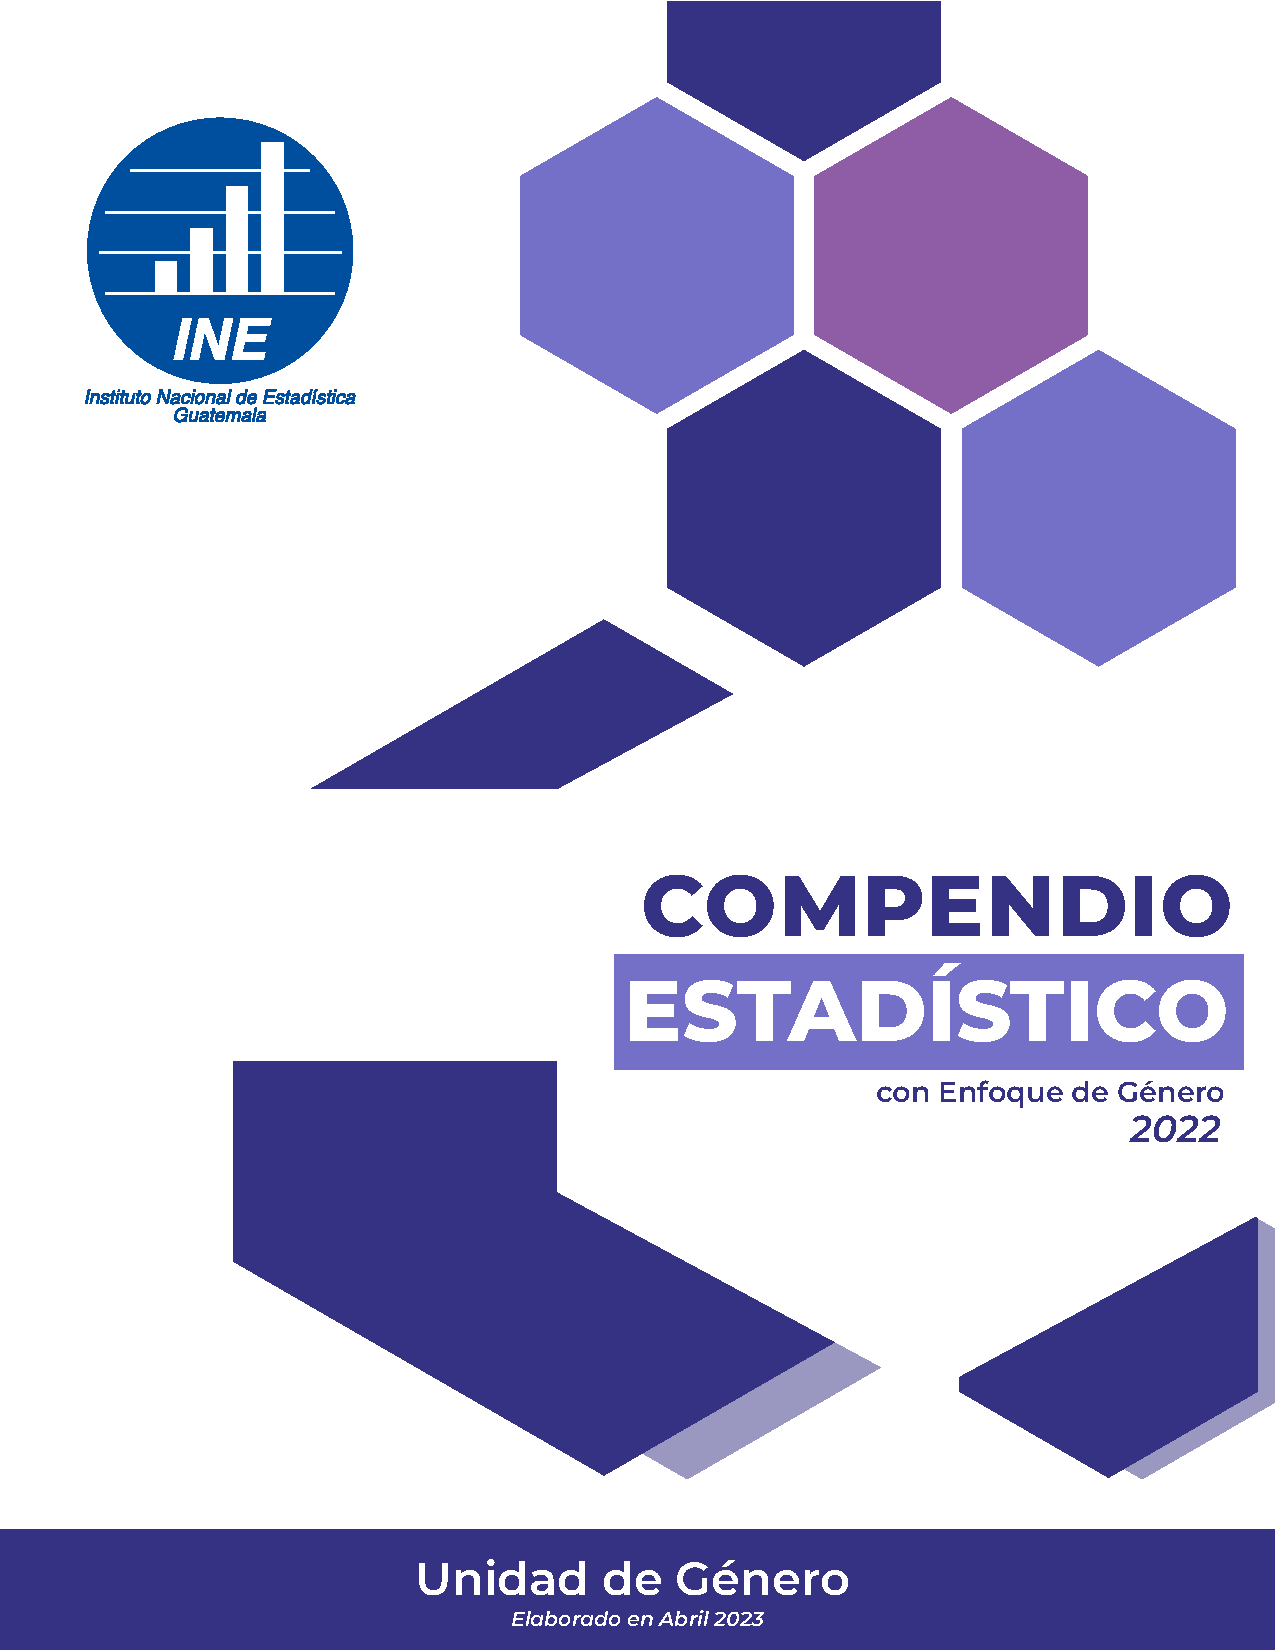
\includepdf{Plantilla/Portada_CEEG_2022.pdf}
	\cleardoublepage
	\thispagestyle{soloarriba}
	\begin{center}
	{\Bold \LARGE AUTORIDADES}\\[1cm]
{\Bold \large \color{color3} JUNTA  DIRECTIVA} \\[0.4cm]
{\Bold Ministerio de Economía}\\ 
Titular: Janio Moacyr Rosales Alegría \\ 
Suplente: Francisca de Jesús Cárdenas Morán\\[0.4cm]

{\Bold Ministerio de Finanzas Públicas}\\ 
Titular: Edwin Oswaldo Martínez Cameros\\ 
Suplente: José Hugo Valle Alegría\\[0.4cm]

{\Bold Ministerio de Agricultura, Ganadería y Alimentación}\\ 
Titular: Edgar René De León Moreno\\ 
Suplente: César Vinicio Arreaga Morales\\[0.4cm]

{\Bold Ministerio de Energía y Minas}\\ 
Titular: Alberto Pimentel Mata\\ 
Suplente: Oscar Rafael Pérez Ramírez\\[0.4cm]

{\Bold Secretaría de Planificación y Programación de la Presidencia}\\ 
Titular: Luz Keila Virginia Gramajo Vilchez\\ 
Suplente: Manuel Augusto Alonzo Araujo\\[0.4cm]

{\Bold Banco de Guatemala}\\ 
Titular: Álvaro González Ricci \\ 
Suplente: José Alfredo Blanco Valdés\\[0.4cm]

{\Bold Universidad de San Carlos de Guatemala}\\ 
Titular: Sindy Massiel Godínez Bautista\\ 
Suplente: José Lara Samayoa\\[0.4cm]

{\Bold Universidades Privadas}\\ 
Titular: Miguel Ángel Franco de León\\ 
Suplente: Oscar Leonel Herrera Velásquez\\[0.4cm]

{\Bold Comité Coordinador de Asociaciones Agrícolas, Comerciales, Industriales y Financieras}\\ 
Titular: Hugo Leonel Maúl Rivas\\ 
Suplente: Ricardo Antonio Rodríguez Martínez\\[0.4cm]

{\Bold \large \color{color3} GERENCIA}\\[0.2cm]
Gerente: Brenda Izabel Miranda Consuegra\\ 
Subgerente Técnico: Hugo Allan García Monterrosa\\ 
Subgerente Administrativo Financiero: Marco Antonio Mejía Villatoro\\ 

	\end{center}
	\cleardoublepage
	$\ $
	\vspace{0.0cm}
	\thispagestyle{soloarriba}
	\begin{center}
	{\Bold \LARGE EQUIPO RESPONSABLE}\\[2cm]
%{\Bold \large \color{color1!89!black} REVISIÓN GENERAL}\\[0.2cm]
%Brenda Izabel Miranda Consuegra\\[0.8cm]
{\Bold \large \color{color1!89!black} EQUIPO TÉCNICO}\\[0.2cm]
Brenda Izabel Miranda Consuegra\\
Hugo Allan García Monterrosa\\
Edgar Edwardo Herrarte Rodríguez\\
Julio Roberto Ramírez Pacheco \\
Luis Fernando Castellanos Bonilla \\
María Eugenia Guzmán Chete\\
Cristian Miguel Cabrera Ayala\\
Marvin Isaac Reyes López\\
Patricia Eugenia Hernandez García\\
Paula Natalia Gálvez Molina\\
Rodrigo Rafael Castillo Chong\\
Gerardo Ernesto Rodríguez\\
Mario Raul Soto Gómez\\
Luis Alberto Peñate López\\[0.8cm]
{\Bold \large \color{color1!89!black} DIAGRAMACIÓN Y DISEÑO}\\[0.2cm]
Andrea Michelle Rojas Salvatierra\\[0.8cm]

	\end{center}
	\cleardoublepage
	$\ $
	\vspace{0.0cm}
	\thispagestyle{soloarriba}
	\begin{center}
{\Bold \LARGE \color{color3} PRESENTACIÓN}\\[2cm]
\end{center}

EN PROCESO
\begin{center}
Brenda Izabel Miranda Consuegra\\
\textbf{Gerente}
\end{center}


	\cleardoublepage
	$\ $\\[2cm]
	\tableofcontents
	\pagestyle{estandar}	
	\vspace{0.0cm}
	\clearpage
	\setcounter{page}{0}
	
\INEchaptercarta{Población y demografía}{Capítulo dedicado a mostrar una composición general de las personas que habitan en el territorio guatemalteco respecto a su tamaño y su estructura de la población diferenciada por sexo, por edad, contribuyendo a la construcción de indicadores de la dinámica demográfica, a nivel nacional con un enfoque de género y pueblos.}
\cajota{Población por sexo, según grupos de edad}{Para el 2022, el grupo de edad de 15 a 19 años tiene la población más grande de los grupos de edad con 956,598.8 miles de personas. El siguiente grupo más poblado es de 0 a 4 años de edad con 1681.9 miles de personas. Por el contrario,  la población de 100 años o más cuenta con la menor cantidad de personas de todos los grupos con 1.2 miles de personas. }{Población por sexo, según grupos de edad (miles de personas), 2022}{República de Guatemala, Instituto Nacional de Estadística}{\begin{tikzpicture}[x=1pt,y=1pt, scale=1.75]% Created by tikzDevice version 0.12.4 on 2023-04-04 13:49:55
% !TEX encoding = UTF-8 Unicode
\definecolor{fillColor}{RGB}{255,255,255}
\path[use as bounding box,fill=fillColor,fill opacity=0.00] (0,0) rectangle (289.08,198.74);
\begin{scope}
\path[clip] (  0.00,  0.00) rectangle (289.08,198.74);
\definecolor{drawColor}{RGB}{255,255,255}
\definecolor{fillColor}{RGB}{255,255,255}

\path[draw=drawColor,line width= 0.6pt,line join=round,line cap=round,fill=fillColor] (  0.00,  0.00) rectangle (289.08,198.74);
\end{scope}
\begin{scope}
\path[clip] (  0.00,  0.00) rectangle (289.08,198.74);
\definecolor{fillColor}{RGB}{54,50,131}

\path[fill=fillColor] ( 49.83, 33.17) rectangle (128.50, 40.01);

\path[fill=fillColor] ( 50.06, 40.77) rectangle (128.50, 47.62);

\path[fill=fillColor] ( 53.08, 48.38) rectangle (128.50, 55.22);

\path[fill=fillColor] ( 47.93, 55.98) rectangle (128.50, 62.83);

\path[fill=fillColor] ( 55.37, 63.59) rectangle (128.50, 70.43);

\path[fill=fillColor] ( 66.82, 71.19) rectangle (128.50, 78.03);

\path[fill=fillColor] ( 77.71, 78.79) rectangle (128.50, 85.64);

\path[fill=fillColor] ( 81.13, 86.40) rectangle (128.50, 93.24);

\path[fill=fillColor] ( 90.24, 94.00) rectangle (128.50,100.85);

\path[fill=fillColor] ( 96.76,101.61) rectangle (128.50,108.45);

\path[fill=fillColor] (101.65,109.21) rectangle (128.50,116.06);

\path[fill=fillColor] (105.47,116.82) rectangle (128.50,123.66);

\path[fill=fillColor] (109.95,124.42) rectangle (128.50,131.27);

\path[fill=fillColor] (113.42,132.03) rectangle (128.50,138.87);

\path[fill=fillColor] (118.19,139.63) rectangle (128.50,146.47);

\path[fill=fillColor] (121.23,147.24) rectangle (128.50,154.08);

\path[fill=fillColor] (123.82,154.84) rectangle (128.50,161.68);

\path[fill=fillColor] (125.59,162.44) rectangle (128.50,169.29);

\path[fill=fillColor] (127.43,170.05) rectangle (128.50,176.89);

\path[fill=fillColor] (128.15,177.65) rectangle (128.50,184.50);

\path[fill=fillColor] (128.43,185.26) rectangle (128.50,192.10);
\definecolor{fillColor}{RGB}{116,112,200}

\path[fill=fillColor] (128.50, 33.17) rectangle (208.89, 40.01);

\path[fill=fillColor] (128.50, 40.77) rectangle (208.64, 47.62);

\path[fill=fillColor] (128.50, 48.38) rectangle (205.73, 55.22);

\path[fill=fillColor] (128.50, 55.98) rectangle (207.08, 62.83);

\path[fill=fillColor] (128.50, 63.59) rectangle (196.62, 70.43);

\path[fill=fillColor] (128.50, 71.19) rectangle (183.82, 78.03);

\path[fill=fillColor] (128.50, 78.79) rectangle (173.20, 85.64);

\path[fill=fillColor] (128.50, 86.40) rectangle (169.09, 93.24);

\path[fill=fillColor] (128.50, 94.00) rectangle (162.08,100.85);

\path[fill=fillColor] (128.50,101.61) rectangle (155.53,108.45);

\path[fill=fillColor] (128.50,109.21) rectangle (152.06,116.06);

\path[fill=fillColor] (128.50,116.82) rectangle (148.32,123.66);

\path[fill=fillColor] (128.50,124.42) rectangle (145.04,131.27);

\path[fill=fillColor] (128.50,132.03) rectangle (141.84,138.87);

\path[fill=fillColor] (128.50,139.63) rectangle (138.12,146.47);

\path[fill=fillColor] (128.50,147.24) rectangle (135.12,154.08);

\path[fill=fillColor] (128.50,154.84) rectangle (132.74,161.68);

\path[fill=fillColor] (128.50,162.44) rectangle (130.97,169.29);

\path[fill=fillColor] (128.50,170.05) rectangle (129.36,176.89);

\path[fill=fillColor] (128.50,177.65) rectangle (128.75,184.50);

\path[fill=fillColor] (128.50,185.26) rectangle (128.54,192.10);
\end{scope}
\begin{scope}
\path[clip] (  0.00,  0.00) rectangle (289.08,198.74);
\definecolor{drawColor}{gray}{0.30}

\node[text=drawColor,anchor=base east,inner sep=0pt, outer sep=0pt, scale=  0.80] at ( 34.93, 33.46) {0-4};

\node[text=drawColor,anchor=base east,inner sep=0pt, outer sep=0pt, scale=  0.80] at ( 34.93, 41.07) {5-9};

\node[text=drawColor,anchor=base east,inner sep=0pt, outer sep=0pt, scale=  0.80] at ( 34.93, 48.67) {10-14};

\node[text=drawColor,anchor=base east,inner sep=0pt, outer sep=0pt, scale=  0.80] at ( 34.93, 56.28) {15-19};

\node[text=drawColor,anchor=base east,inner sep=0pt, outer sep=0pt, scale=  0.80] at ( 34.93, 63.88) {20-24};

\node[text=drawColor,anchor=base east,inner sep=0pt, outer sep=0pt, scale=  0.80] at ( 34.93, 71.49) {25-29};

\node[text=drawColor,anchor=base east,inner sep=0pt, outer sep=0pt, scale=  0.80] at ( 34.93, 79.09) {30-34};

\node[text=drawColor,anchor=base east,inner sep=0pt, outer sep=0pt, scale=  0.80] at ( 34.93, 86.69) {35-39};

\node[text=drawColor,anchor=base east,inner sep=0pt, outer sep=0pt, scale=  0.80] at ( 34.93, 94.30) {40-44};

\node[text=drawColor,anchor=base east,inner sep=0pt, outer sep=0pt, scale=  0.80] at ( 34.93,101.90) {45-49};

\node[text=drawColor,anchor=base east,inner sep=0pt, outer sep=0pt, scale=  0.80] at ( 34.93,109.51) {50-54};

\node[text=drawColor,anchor=base east,inner sep=0pt, outer sep=0pt, scale=  0.80] at ( 34.93,117.11) {55-59};

\node[text=drawColor,anchor=base east,inner sep=0pt, outer sep=0pt, scale=  0.80] at ( 34.93,124.72) {60-64};

\node[text=drawColor,anchor=base east,inner sep=0pt, outer sep=0pt, scale=  0.80] at ( 34.93,132.32) {65-69};

\node[text=drawColor,anchor=base east,inner sep=0pt, outer sep=0pt, scale=  0.80] at ( 34.93,139.93) {70-74};

\node[text=drawColor,anchor=base east,inner sep=0pt, outer sep=0pt, scale=  0.80] at ( 34.93,147.53) {75-79};

\node[text=drawColor,anchor=base east,inner sep=0pt, outer sep=0pt, scale=  0.80] at ( 34.93,155.14) {80-84};

\node[text=drawColor,anchor=base east,inner sep=0pt, outer sep=0pt, scale=  0.80] at ( 34.93,162.74) {85-89};

\node[text=drawColor,anchor=base east,inner sep=0pt, outer sep=0pt, scale=  0.80] at ( 34.93,170.34) {90-94};

\node[text=drawColor,anchor=base east,inner sep=0pt, outer sep=0pt, scale=  0.80] at ( 34.93,177.95) {95-99};

\node[text=drawColor,anchor=base east,inner sep=0pt, outer sep=0pt, scale=  0.80] at ( 34.93,185.55) {100+};
\end{scope}
\begin{scope}
\path[clip] (  0.00,  0.00) rectangle (289.08,198.74);
\definecolor{drawColor}{gray}{0.20}

\path[draw=drawColor,line width= 0.6pt,line join=round] ( 37.13, 36.59) --
	( 39.88, 36.59);

\path[draw=drawColor,line width= 0.6pt,line join=round] ( 37.13, 44.19) --
	( 39.88, 44.19);

\path[draw=drawColor,line width= 0.6pt,line join=round] ( 37.13, 51.80) --
	( 39.88, 51.80);

\path[draw=drawColor,line width= 0.6pt,line join=round] ( 37.13, 59.40) --
	( 39.88, 59.40);

\path[draw=drawColor,line width= 0.6pt,line join=round] ( 37.13, 67.01) --
	( 39.88, 67.01);

\path[draw=drawColor,line width= 0.6pt,line join=round] ( 37.13, 74.61) --
	( 39.88, 74.61);

\path[draw=drawColor,line width= 0.6pt,line join=round] ( 37.13, 82.22) --
	( 39.88, 82.22);

\path[draw=drawColor,line width= 0.6pt,line join=round] ( 37.13, 89.82) --
	( 39.88, 89.82);

\path[draw=drawColor,line width= 0.6pt,line join=round] ( 37.13, 97.43) --
	( 39.88, 97.43);

\path[draw=drawColor,line width= 0.6pt,line join=round] ( 37.13,105.03) --
	( 39.88,105.03);

\path[draw=drawColor,line width= 0.6pt,line join=round] ( 37.13,112.63) --
	( 39.88,112.63);

\path[draw=drawColor,line width= 0.6pt,line join=round] ( 37.13,120.24) --
	( 39.88,120.24);

\path[draw=drawColor,line width= 0.6pt,line join=round] ( 37.13,127.84) --
	( 39.88,127.84);

\path[draw=drawColor,line width= 0.6pt,line join=round] ( 37.13,135.45) --
	( 39.88,135.45);

\path[draw=drawColor,line width= 0.6pt,line join=round] ( 37.13,143.05) --
	( 39.88,143.05);

\path[draw=drawColor,line width= 0.6pt,line join=round] ( 37.13,150.66) --
	( 39.88,150.66);

\path[draw=drawColor,line width= 0.6pt,line join=round] ( 37.13,158.26) --
	( 39.88,158.26);

\path[draw=drawColor,line width= 0.6pt,line join=round] ( 37.13,165.87) --
	( 39.88,165.87);

\path[draw=drawColor,line width= 0.6pt,line join=round] ( 37.13,173.47) --
	( 39.88,173.47);

\path[draw=drawColor,line width= 0.6pt,line join=round] ( 37.13,181.08) --
	( 39.88,181.08);

\path[draw=drawColor,line width= 0.6pt,line join=round] ( 37.13,188.68) --
	( 39.88,188.68);
\end{scope}
\begin{scope}
\path[clip] (  0.00,  0.00) rectangle (289.08,198.74);
\definecolor{drawColor}{gray}{0.20}

\path[draw=drawColor,line width= 0.6pt,line join=round] ( 47.93, 29.28) --
	( 47.93, 32.03);

\path[draw=drawColor,line width= 0.6pt,line join=round] ( 88.21, 29.28) --
	( 88.21, 32.03);

\path[draw=drawColor,line width= 0.6pt,line join=round] (128.50, 29.28) --
	(128.50, 32.03);

\path[draw=drawColor,line width= 0.6pt,line join=round] (168.69, 29.28) --
	(168.69, 32.03);

\path[draw=drawColor,line width= 0.6pt,line join=round] (208.89, 29.28) --
	(208.89, 32.03);
\end{scope}
\begin{scope}
\path[clip] (  0.00,  0.00) rectangle (289.08,198.74);
\definecolor{drawColor}{gray}{0.30}

\node[text=drawColor,anchor=base,inner sep=0pt, outer sep=0pt, scale=  0.80] at ( 47.93, 20.82) {851.9};

\node[text=drawColor,anchor=base,inner sep=0pt, outer sep=0pt, scale=  0.80] at ( 88.21, 20.82) {426};

\node[text=drawColor,anchor=base,inner sep=0pt, outer sep=0pt, scale=  0.80] at (128.50, 20.82) {0};

\node[text=drawColor,anchor=base,inner sep=0pt, outer sep=0pt, scale=  0.80] at (168.69, 20.82) {425};

\node[text=drawColor,anchor=base,inner sep=0pt, outer sep=0pt, scale=  0.80] at (208.89, 20.82) {850.1};
\end{scope}
\begin{scope}
\path[clip] (  0.00,  0.00) rectangle (289.08,198.74);
\definecolor{drawColor}{RGB}{0,0,0}

\node[text=drawColor,anchor=base,inner sep=0pt, outer sep=0pt, scale=  1.00] at (128.41,  8.14) {Población en miles de personas};
\end{scope}
\begin{scope}
\path[clip] (  0.00,  0.00) rectangle (289.08,198.74);
\definecolor{drawColor}{RGB}{0,0,0}

\node[text=drawColor,rotate= 90.00,anchor=base,inner sep=0pt, outer sep=0pt, scale=  1.00] at ( 13.32,112.63) {Grupo de edad};
\end{scope}
\begin{scope}
\path[clip] (  0.00,  0.00) rectangle (289.08,198.74);
\definecolor{fillColor}{RGB}{255,255,255}

\path[fill=fillColor] (227.94, 83.26) rectangle (283.58,142.01);
\end{scope}
\begin{scope}
\path[clip] (  0.00,  0.00) rectangle (289.08,198.74);
\definecolor{drawColor}{RGB}{0,0,0}

\node[text=drawColor,anchor=base west,inner sep=0pt, outer sep=0pt, scale=  1.00] at (233.44,127.38) {Sexo};
\end{scope}
\begin{scope}
\path[clip] (  0.00,  0.00) rectangle (289.08,198.74);
\definecolor{fillColor}{gray}{0.95}

\path[fill=fillColor] (233.44,104.66) rectangle (249.34,120.55);
\end{scope}
\begin{scope}
\path[clip] (  0.00,  0.00) rectangle (289.08,198.74);
\definecolor{fillColor}{RGB}{54,50,131}

\path[fill=fillColor] (234.15,105.37) rectangle (248.63,119.84);
\end{scope}
\begin{scope}
\path[clip] (  0.00,  0.00) rectangle (289.08,198.74);
\definecolor{fillColor}{gray}{0.95}

\path[fill=fillColor] (233.44, 88.76) rectangle (249.34,104.66);
\end{scope}
\begin{scope}
\path[clip] (  0.00,  0.00) rectangle (289.08,198.74);
\definecolor{fillColor}{RGB}{116,112,200}

\path[fill=fillColor] (234.15, 89.47) rectangle (248.63,103.94);
\end{scope}
\begin{scope}
\path[clip] (  0.00,  0.00) rectangle (289.08,198.74);
\definecolor{drawColor}{RGB}{0,0,0}

\node[text=drawColor,anchor=base west,inner sep=0pt, outer sep=0pt, scale=  0.80] at (254.84,109.48) {Mujer};
\end{scope}
\begin{scope}
\path[clip] (  0.00,  0.00) rectangle (289.08,198.74);
\definecolor{drawColor}{RGB}{0,0,0}

\node[text=drawColor,anchor=base west,inner sep=0pt, outer sep=0pt, scale=  0.80] at (254.84, 93.58) {Hombre};
\end{scope}
\end{tikzpicture}}{INE - Proyecciones 2020} %1

\cajita{Población por sexo, según dominio de estudio}{Para 2022, según las proyecciones de población del Instituto Nacional de Estadística, en la República de Guatemala habitaban 17,357,886 personas. }{Población por sexo, según dominio de estudio (porcentaje), 2022}{República de Guatemala, Instituto Nacional de Estadística}{\begin{tikzpicture}[x=1pt,y=1pt, scale = 1.25]% Created by tikzDevice version 0.12.4 on 2023-04-20 12:31:17
% !TEX encoding = UTF-8 Unicode
\end{tikzpicture}}{INE - ENEI 2022}{} %2

\cajita{Población por sexo, según Pueblos}{Para 2022, el 31.2\% de la población guatemalteca estaba compuesta por mujeres ladinas. El 27.8\% eran hombres ladinos, y el 19.6\% mujeres mayas. El 0.1\% eran mujeres garífunas, otro 0.1\% hombres garífunas, y 0.1\% mujeres extranjeras. \footnote{Afrodescendiente*: Afrodescendiente/Creole/Afro mestizo.}}{Población por sexo, según Pueblos (porcentaje), 2022}{República de Guatemala, Instituto Nacional de Estadística}{\begin{tikzpicture}[x=1pt,y=1pt]% Created by tikzDevice version 0.12.4 on 2023-05-02 12:30:50
% !TEX encoding = UTF-8 Unicode
\definecolor{fillColor}{RGB}{255,255,255}
\path[use as bounding box,fill=fillColor,fill opacity=0.00] (0,0) rectangle (289.08,198.74);
\begin{scope}
\path[clip] (  0.00,  0.00) rectangle (289.08,198.74);

\path[] (  0.00,  0.00) rectangle (289.08,198.74);
\end{scope}
\begin{scope}
\path[clip] (  0.00,  0.00) rectangle (289.08,198.74);
\definecolor{fillColor}{RGB}{54,50,131}

\path[fill=fillColor] ( 80.50,171.20) rectangle ( 85.23,183.01);

\path[fill=fillColor] ( 80.50, 92.52) rectangle ( 81.24,104.32);

\path[fill=fillColor] ( 80.50,118.75) rectangle (279.15,130.55);

\path[fill=fillColor] ( 80.50, 40.07) rectangle ( 88.59, 51.87);

\path[fill=fillColor] ( 80.50, 66.29) rectangle ( 81.13, 78.10);

\path[fill=fillColor] ( 80.50,144.98) rectangle (205.38,156.78);
\definecolor{fillColor}{RGB}{116,112,200}

\path[fill=fillColor] ( 80.50,183.01) rectangle ( 84.35,194.81);

\path[fill=fillColor] ( 80.50,104.32) rectangle ( 81.11,116.13);

\path[fill=fillColor] ( 80.50,130.55) rectangle (257.44,142.35);

\path[fill=fillColor] ( 80.50, 51.87) rectangle ( 89.16, 63.67);

\path[fill=fillColor] ( 80.50, 78.10) rectangle ( 81.45, 89.90);

\path[fill=fillColor] ( 80.50,156.78) rectangle (188.23,168.58);
\definecolor{drawColor}{RGB}{0,0,0}

\node[text=drawColor,anchor=base west,inner sep=0pt, outer sep=0pt, scale=  0.68] at ( 89.50,173.42) {0.7};

\node[text=drawColor,anchor=base west,inner sep=0pt, outer sep=0pt, scale=  0.68] at ( 85.51, 94.73) {0.1};

\node[text=drawColor,anchor=base west,inner sep=0pt, outer sep=0pt, scale=  0.68] at (279.12,120.96) {31.2};

\node[text=drawColor,anchor=base west,inner sep=0pt, outer sep=0pt, scale=  0.63] at ( 92.86, 42.28) {1.3};

\node[text=drawColor,anchor=base west,inner sep=0pt, outer sep=0pt, scale=  0.63] at ( 85.40, 68.51) {0.1};

\node[text=drawColor,anchor=base west,inner sep=0pt, outer sep=0pt, scale=  0.63] at (211.36,147.19) {19.6};

\node[text=drawColor,anchor=base west,inner sep=0pt, outer sep=0pt, scale=  0.63] at ( 88.62,186.53) {0.6};

\node[text=drawColor,anchor=base west,inner sep=0pt, outer sep=0pt, scale=  0.63] at ( 85.38,107.85) {0.1};

\node[text=drawColor,anchor=base west,inner sep=0pt, outer sep=0pt, scale=  0.63] at (263.41,134.07) {27.8};

\node[text=drawColor,anchor=base west,inner sep=0pt, outer sep=0pt, scale=  0.63] at ( 93.44, 55.39) {1.4};

\node[text=drawColor,anchor=base west,inner sep=0pt, outer sep=0pt, scale=  0.63] at ( 85.73, 81.62) {0.2};

\node[text=drawColor,anchor=base west,inner sep=0pt, outer sep=0pt, scale=  0.63] at (194.20,160.30) {16.9};

\path[] ( 70.56, 51.87) --
	(289.08, 51.87);

\path[] ( 70.56, 78.10) --
	(289.08, 78.10);

\path[] ( 70.56,104.32) --
	(289.08,104.32);

\path[] ( 70.56,130.55) --
	(289.08,130.55);

\path[] ( 70.56,156.78) --
	(289.08,156.78);

\path[] ( 70.56,183.01) --
	(289.08,183.01);

\path[] ( 70.56, 36.13) rectangle (289.08,198.74);
\end{scope}
\begin{scope}
\path[clip] (  0.00,  0.00) rectangle (289.08,198.74);

\path[] ( 70.56, 36.13) --
	( 70.56,198.74);
\end{scope}
\begin{scope}
\path[clip] (  0.00,  0.00) rectangle (289.08,198.74);
\definecolor{drawColor}{RGB}{0,0,0}

\node[text=drawColor,anchor=base east,inner sep=0pt, outer sep=0pt, scale=  1.00] at ( 65.61, 47.96) {Afrodescendiente*};

\node[text=drawColor,anchor=base east,inner sep=0pt, outer sep=0pt, scale=  1.00] at ( 65.61, 74.19) {Extranjero};

\node[text=drawColor,anchor=base east,inner sep=0pt, outer sep=0pt, scale=  1.00] at ( 65.61,100.41) {Garífuna};

\node[text=drawColor,anchor=base east,inner sep=0pt, outer sep=0pt, scale=  1.00] at ( 65.61,126.64) {Ladino};

\node[text=drawColor,anchor=base east,inner sep=0pt, outer sep=0pt, scale=  1.00] at ( 65.61,152.87) {Maya};

\node[text=drawColor,anchor=base east,inner sep=0pt, outer sep=0pt, scale=  1.00] at ( 65.61,179.10) {Xinka};
\end{scope}
\begin{scope}
\path[clip] (  0.00,  0.00) rectangle (289.08,198.74);

\path[] ( 67.81, 51.87) --
	( 70.56, 51.87);

\path[] ( 67.81, 78.10) --
	( 70.56, 78.10);

\path[] ( 67.81,104.32) --
	( 70.56,104.32);

\path[] ( 67.81,130.55) --
	( 70.56,130.55);

\path[] ( 67.81,156.78) --
	( 70.56,156.78);

\path[] ( 67.81,183.01) --
	( 70.56,183.01);
\end{scope}
\begin{scope}
\path[clip] (  0.00,  0.00) rectangle (289.08,198.74);

\path[] ( 70.56, 36.13) --
	(289.08, 36.13);
\end{scope}
\begin{scope}
\path[clip] (  0.00,  0.00) rectangle (289.08,198.74);

\path[] ( 80.50, 33.38) --
	( 80.50, 36.13);

\path[] (144.15, 33.38) --
	(144.15, 36.13);

\path[] (207.80, 33.38) --
	(207.80, 36.13);

\path[] (271.45, 33.38) --
	(271.45, 36.13);
\end{scope}
\begin{scope}
\path[clip] (  0.00,  0.00) rectangle (289.08,198.74);
\definecolor{fillColor}{RGB}{255,255,255}

\path[fill=fillColor] (131.74, -0.00) rectangle (227.91, 22.38);
\end{scope}
\begin{scope}
\path[clip] (  0.00,  0.00) rectangle (289.08,198.74);
\definecolor{fillColor}{gray}{0.95}

\path[fill=fillColor] (132.74,  5.50) rectangle (144.12, 16.88);
\end{scope}
\begin{scope}
\path[clip] (  0.00,  0.00) rectangle (289.08,198.74);
\definecolor{fillColor}{RGB}{54,50,131}

\path[fill=fillColor] (133.40,  6.16) rectangle (143.46, 16.22);  %cuadro leyenda mujeres
\end{scope}
\begin{scope}
\path[clip] (  0.00,  0.00) rectangle (289.08,198.74);
\definecolor{fillColor}{gray}{0.95}

\path[fill=fillColor] (182.28,  5.50) rectangle (193.66, 16.88);
\end{scope}
\begin{scope}
\path[clip] (  0.00,  0.00) rectangle (289.08,198.74);
\definecolor{fillColor}{RGB}{116,112,200}

\path[fill=fillColor] (182.94,  6.16) rectangle (193.00, 16.22);
\end{scope}
\begin{scope}
\path[clip] (  0.00,  0.00) rectangle (289.08,198.74);
\definecolor{drawColor}{RGB}{0,0,0}

\node[text=drawColor,anchor=base west,inner sep=0pt, outer sep=0pt, scale=  0.80] at (149.62,  8.06) {Mujeres};
\end{scope}
\begin{scope}
\path[clip] (  0.00,  0.00) rectangle (289.08,198.74);
\definecolor{drawColor}{RGB}{0,0,0}

\node[text=drawColor,anchor=base west,inner sep=0pt, outer sep=0pt, scale=  0.80] at (199.16,  8.06) {Hombres};
\end{scope}
\end{tikzpicture}}{INE - ENEI 2022}{} %3

\cajota{Población por sexo, según comunidad lingüística}{Para el 2018, se muestra el número de personas por sexo pertenecientes a las 22 comunidades lingüísticas Maya. Se observa que en la mayoría de comunidades existe una mayor población de mujeres, con excepción de la comunidad Itza’.}{Población por sexo, según comunidad lingüística (número de personas), 2018}{República de Guatemala, Instituto Nacional de Estadística}{\begin{tikzpicture}[x=1pt,y=1pt, scale=1.75]% Created by tikzDevice version 0.12.4 on 2023-05-08 10:54:28
% !TEX encoding = UTF-8 Unicode
\definecolor{fillColor}{RGB}{255,255,255}
\path[use as bounding box,fill=fillColor,fill opacity=0.00] (0,0) rectangle (289.08,198.74);
\begin{scope}
\path[clip] (  0.00,  0.00) rectangle (289.08,198.74);
\definecolor{drawColor}{RGB}{255,255,255}
\definecolor{fillColor}{RGB}{255,255,255}

\path[draw=drawColor,line width= 0.6pt,line join=round,line cap=round,fill=fillColor] (  0.00,  0.00) rectangle (289.08,198.74);
\end{scope}
\begin{scope}
\path[clip] (  0.00,  0.00) rectangle (289.08,198.74);
\definecolor{fillColor}{RGB}{54,50,131}

\path[fill=fillColor] (134.05,  6.77) rectangle (213.87, 14.38);

\path[fill=fillColor] (137.61, 15.23) rectangle (213.87, 22.84);

\path[fill=fillColor] (131.67, 23.68) rectangle (213.87, 31.29);

\path[fill=fillColor] (136.88, 32.14) rectangle (213.87, 39.75);

\path[fill=fillColor] (133.91, 40.60) rectangle (213.87, 48.21);

\path[fill=fillColor] (135.04, 49.05) rectangle (213.87, 56.66);

\path[fill=fillColor] (141.56, 57.51) rectangle (213.87, 65.12);

\path[fill=fillColor] (134.14, 65.97) rectangle (213.87, 73.58);

\path[fill=fillColor] (132.55, 74.42) rectangle (213.87, 82.03);

\path[fill=fillColor] (134.24, 82.88) rectangle (213.87, 90.49);

\path[fill=fillColor] (136.05, 91.34) rectangle (213.87, 98.95);

\path[fill=fillColor] (133.87, 99.79) rectangle (213.87,107.41);

\path[fill=fillColor] (137.35,108.25) rectangle (213.87,115.86);

\path[fill=fillColor] (135.08,116.71) rectangle (213.87,124.32);

\path[fill=fillColor] (137.45,125.16) rectangle (213.87,132.78);

\path[fill=fillColor] (134.62,133.62) rectangle (213.87,141.23);

\path[fill=fillColor] (137.98,142.08) rectangle (213.87,149.69);

\path[fill=fillColor] (133.67,150.54) rectangle (213.87,158.15);

\path[fill=fillColor] (136.52,158.99) rectangle (213.87,166.60);

\path[fill=fillColor] (135.40,167.45) rectangle (213.87,175.06);

\path[fill=fillColor] (137.08,175.91) rectangle (213.87,183.52);

\path[fill=fillColor] (134.83,184.36) rectangle (213.87,191.97);
\definecolor{fillColor}{RGB}{116,112,200}

\path[fill=fillColor] ( 62.19,  6.77) rectangle (134.05, 14.38);

\path[fill=fillColor] ( 62.19, 15.23) rectangle (137.61, 22.84);

\path[fill=fillColor] ( 62.19, 23.68) rectangle (131.67, 31.29);

\path[fill=fillColor] ( 62.19, 32.14) rectangle (136.88, 39.75);

\path[fill=fillColor] ( 62.19, 40.60) rectangle (133.91, 48.21);

\path[fill=fillColor] ( 62.19, 49.05) rectangle (135.04, 56.66);

\path[fill=fillColor] ( 62.19, 57.51) rectangle (141.56, 65.12);

\path[fill=fillColor] ( 62.19, 65.97) rectangle (134.14, 73.58);

\path[fill=fillColor] ( 62.19, 74.42) rectangle (132.55, 82.03);

\path[fill=fillColor] ( 62.19, 82.88) rectangle (134.24, 90.49);

\path[fill=fillColor] ( 62.19, 91.34) rectangle (136.05, 98.95);

\path[fill=fillColor] ( 62.19, 99.79) rectangle (133.87,107.41);

\path[fill=fillColor] ( 62.19,108.25) rectangle (137.35,115.86);

\path[fill=fillColor] ( 62.19,116.71) rectangle (135.08,124.32);

\path[fill=fillColor] ( 62.19,125.16) rectangle (137.45,132.78);

\path[fill=fillColor] ( 62.19,133.62) rectangle (134.62,141.23);

\path[fill=fillColor] ( 62.19,142.08) rectangle (137.98,149.69);

\path[fill=fillColor] ( 62.19,150.54) rectangle (133.67,158.15);

\path[fill=fillColor] ( 62.19,158.99) rectangle (136.52,166.60);

\path[fill=fillColor] ( 62.19,167.45) rectangle (135.40,175.06);

\path[fill=fillColor] ( 62.19,175.91) rectangle (137.08,183.52);

\path[fill=fillColor] ( 62.19,184.36) rectangle (134.83,191.97);
\definecolor{drawColor}{RGB}{255,255,255}

\node[text=drawColor,anchor=base,inner sep=0pt, outer sep=0pt, scale=  0.78] at (173.96,  7.54) {84,649};

\node[text=drawColor,anchor=base,inner sep=0pt, outer sep=0pt, scale=  0.78] at (175.74, 16.00) {33,167};

\node[text=drawColor,anchor=base,inner sep=0pt, outer sep=0pt, scale=  0.78] at (172.77, 24.45) {6,796};

\node[text=drawColor,anchor=base,inner sep=0pt, outer sep=0pt, scale=  0.78] at (175.37, 32.91) {57,071};

\node[text=drawColor,anchor=base,inner sep=0pt, outer sep=0pt, scale=  0.78] at (173.89, 41.37) {17,735};

\node[text=drawColor,anchor=base,inner sep=0pt, outer sep=0pt, scale=  0.78] at (174.46, 49.83) {47,496};

\node[text=drawColor,anchor=base,inner sep=0pt, outer sep=0pt, scale=  0.78] at (177.71, 58.28) {1,395};

\node[text=drawColor,anchor=base,inner sep=0pt, outer sep=0pt, scale=  0.78] at (174.00, 66.74) {70,087};

\node[text=drawColor,anchor=base,inner sep=0pt, outer sep=0pt, scale=  0.78] at (173.21, 75.20) {29,077};

\node[text=drawColor,anchor=base,inner sep=0pt, outer sep=0pt, scale=  0.78] at (174.06, 83.65) {882,288};

\node[text=drawColor,anchor=base,inner sep=0pt, outer sep=0pt, scale=  0.78] at (174.96, 92.11) {548,134};

\node[text=drawColor,anchor=base,inner sep=0pt, outer sep=0pt, scale=  0.78] at (173.87,100.57) {444,217};

\node[text=drawColor,anchor=base,inner sep=0pt, outer sep=0pt, scale=  0.78] at (175.61,109.02) {1,695};

\node[text=drawColor,anchor=base,inner sep=0pt, outer sep=0pt, scale=  0.78] at (174.47,117.48) {24,144};

\node[text=drawColor,anchor=base,inner sep=0pt, outer sep=0pt, scale=  0.78] at (175.66,125.94) {88,987};

\node[text=drawColor,anchor=base,inner sep=0pt, outer sep=0pt, scale=  0.78] at (174.25,134.39) {108,680};

\node[text=drawColor,anchor=base,inner sep=0pt, outer sep=0pt, scale=  0.78] at (175.92,142.85) {685,495};

\node[text=drawColor,anchor=base,inner sep=0pt, outer sep=0pt, scale=  0.78] at (173.77,151.31) {6,841};

\node[text=drawColor,anchor=base,inner sep=0pt, outer sep=0pt, scale=  0.78] at (175.19,159.76) {8,860};

\node[text=drawColor,anchor=base,inner sep=0pt, outer sep=0pt, scale=  0.78] at (174.64,168.22) {1,716};

\node[text=drawColor,anchor=base,inner sep=0pt, outer sep=0pt, scale=  0.78] at (175.48,176.68) {53,668};

\node[text=drawColor,anchor=base,inner sep=0pt, outer sep=0pt, scale=  0.78] at (174.35,185.14) {2,558};

\node[text=drawColor,anchor=base,inner sep=0pt, outer sep=0pt, scale=  0.78] at ( 98.12,  7.54) {76,209};

\node[text=drawColor,anchor=base,inner sep=0pt, outer sep=0pt, scale=  0.78] at ( 99.90, 16.00) {32,798};

\node[text=drawColor,anchor=base,inner sep=0pt, outer sep=0pt, scale=  0.78] at ( 96.93, 24.45) {5,745};

\node[text=drawColor,anchor=base,inner sep=0pt, outer sep=0pt, scale=  0.78] at ( 99.53, 32.91) {55,361};

\node[text=drawColor,anchor=base,inner sep=0pt, outer sep=0pt, scale=  0.78] at ( 98.05, 41.37) {15,906};

\node[text=drawColor,anchor=base,inner sep=0pt, outer sep=0pt, scale=  0.78] at ( 98.62, 49.83) {43,895};

\node[text=drawColor,anchor=base,inner sep=0pt, outer sep=0pt, scale=  0.78] at (101.87, 58.28) {1,531};

\node[text=drawColor,anchor=base,inner sep=0pt, outer sep=0pt, scale=  0.78] at ( 98.16, 66.74) {63,242};

\node[text=drawColor,anchor=base,inner sep=0pt, outer sep=0pt, scale=  0.78] at ( 97.37, 75.20) {25,160};

\node[text=drawColor,anchor=base,inner sep=0pt, outer sep=0pt, scale=  0.78] at ( 98.21, 83.65) {798,263};

\node[text=drawColor,anchor=base,inner sep=0pt, outer sep=0pt, scale=  0.78] at ( 99.12, 92.11) {520,222};

\node[text=drawColor,anchor=base,inner sep=0pt, outer sep=0pt, scale=  0.78] at ( 98.03,100.57) {398,035};

\node[text=drawColor,anchor=base,inner sep=0pt, outer sep=0pt, scale=  0.78] at ( 99.77,109.02) {1,665};

\node[text=drawColor,anchor=base,inner sep=0pt, outer sep=0pt, scale=  0.78] at ( 98.63,117.48) {22,334};

\node[text=drawColor,anchor=base,inner sep=0pt, outer sep=0pt, scale=  0.78] at ( 99.82,125.94) {87,635};

\node[text=drawColor,anchor=base,inner sep=0pt, outer sep=0pt, scale=  0.78] at ( 98.40,134.39) {99,328};

\node[text=drawColor,anchor=base,inner sep=0pt, outer sep=0pt, scale=  0.78] at (100.08,142.85) {684,512};

\node[text=drawColor,anchor=base,inner sep=0pt, outer sep=0pt, scale=  0.78] at ( 97.93,151.31) {6,097};

\node[text=drawColor,anchor=base,inner sep=0pt, outer sep=0pt, scale=  0.78] at ( 99.35,159.76) {8,513};

\node[text=drawColor,anchor=base,inner sep=0pt, outer sep=0pt, scale=  0.78] at ( 98.80,168.22) {1,601};

\node[text=drawColor,anchor=base,inner sep=0pt, outer sep=0pt, scale=  0.78] at ( 99.64,176.68) {52,344};

\node[text=drawColor,anchor=base,inner sep=0pt, outer sep=0pt, scale=  0.78] at ( 98.51,185.14) {2,351};
\end{scope}
\begin{scope}
\path[clip] (  0.00,  0.00) rectangle (289.08,198.74);
\definecolor{drawColor}{RGB}{0,0,0}

\node[text=drawColor,anchor=base east,inner sep=0pt, outer sep=0pt, scale=  0.80] at ( 49.66,  7.45) {Achi};

\node[text=drawColor,anchor=base east,inner sep=0pt, outer sep=0pt, scale=  0.80] at ( 49.66, 15.90) {Akateka};

\node[text=drawColor,anchor=base east,inner sep=0pt, outer sep=0pt, scale=  0.80] at ( 49.66, 24.36) {Awakateka};

\node[text=drawColor,anchor=base east,inner sep=0pt, outer sep=0pt, scale=  0.80] at ( 49.66, 32.82) {Ch'orti'};

\node[text=drawColor,anchor=base east,inner sep=0pt, outer sep=0pt, scale=  0.80] at ( 49.66, 41.27) {Chalchiteka};

\node[text=drawColor,anchor=base east,inner sep=0pt, outer sep=0pt, scale=  0.80] at ( 49.66, 49.73) {Chuj};

\node[text=drawColor,anchor=base east,inner sep=0pt, outer sep=0pt, scale=  0.80] at ( 49.66, 58.19) {Itza'};

\node[text=drawColor,anchor=base east,inner sep=0pt, outer sep=0pt, scale=  0.80] at ( 49.66, 66.65) {Ixil};

\node[text=drawColor,anchor=base east,inner sep=0pt, outer sep=0pt, scale=  0.80] at ( 49.66, 75.10) {Jakalteko/Popti'};

\node[text=drawColor,anchor=base east,inner sep=0pt, outer sep=0pt, scale=  0.80] at ( 49.66, 83.56) {K'iche'};

\node[text=drawColor,anchor=base east,inner sep=0pt, outer sep=0pt, scale=  0.80] at ( 49.66, 92.02) {Kaqchiquel};

\node[text=drawColor,anchor=base east,inner sep=0pt, outer sep=0pt, scale=  0.80] at ( 49.66,100.47) {Mam};

\node[text=drawColor,anchor=base east,inner sep=0pt, outer sep=0pt, scale=  0.80] at ( 49.66,108.93) {Mopan};

\node[text=drawColor,anchor=base east,inner sep=0pt, outer sep=0pt, scale=  0.80] at ( 49.66,117.39) {Poqomam};

\node[text=drawColor,anchor=base east,inner sep=0pt, outer sep=0pt, scale=  0.80] at ( 49.66,125.84) {Poqomchi'};

\node[text=drawColor,anchor=base east,inner sep=0pt, outer sep=0pt, scale=  0.80] at ( 49.66,134.30) {Q'anjob'al};

\node[text=drawColor,anchor=base east,inner sep=0pt, outer sep=0pt, scale=  0.80] at ( 49.66,142.76) {Q'eqchi'};

\node[text=drawColor,anchor=base east,inner sep=0pt, outer sep=0pt, scale=  0.80] at ( 49.66,151.21) {Sakapulteka};

\node[text=drawColor,anchor=base east,inner sep=0pt, outer sep=0pt, scale=  0.80] at ( 49.66,159.67) {Sipakapense};

\node[text=drawColor,anchor=base east,inner sep=0pt, outer sep=0pt, scale=  0.80] at ( 49.66,168.13) {Tektiteka};

\node[text=drawColor,anchor=base east,inner sep=0pt, outer sep=0pt, scale=  0.80] at ( 49.66,176.58) {Tz'utujil};

\node[text=drawColor,anchor=base east,inner sep=0pt, outer sep=0pt, scale=  0.80] at ( 49.66,185.04) {Uspanteka};
\end{scope}
\begin{scope}
\path[clip] (  0.00,  0.00) rectangle (289.08,198.74);
\definecolor{fillColor}{RGB}{255,255,255}

\path[fill=fillColor] (232.46, 74.52) rectangle (283.58,124.23);
\end{scope}
\begin{scope}
\path[clip] (  0.00,  0.00) rectangle (289.08,198.74);
\definecolor{fillColor}{gray}{0.95}

%\path[fill=fillColor] (237.96, 91.40) rectangle (249.34,102.78);
\end{scope}
\begin{scope}
\path[clip] (  0.00,  0.00) rectangle (289.08,198.74);
\definecolor{fillColor}{RGB}{54,50,131}

\path[fill=fillColor] (240.62, 94.06) rectangle (248.67,102.12);
\end{scope}
\begin{scope}
\path[clip] (  0.00,  0.00) rectangle (289.08,198.74);
\definecolor{fillColor}{gray}{0.95}

%\path[fill=fillColor] (237.96, 80.02) rectangle (249.34, 91.40);
\end{scope}
\begin{scope}
\path[clip] (  0.00,  0.00) rectangle (289.08,198.74);
\definecolor{fillColor}{RGB}{116,112,200}

\path[fill=fillColor] (240.62, 84.68) rectangle (248.67, 92.74);
\end{scope}
\begin{scope}
\path[clip] (  0.00,  0.00) rectangle (289.08,198.74);
\definecolor{drawColor}{RGB}{0,0,0}

\node[text=drawColor,anchor=base west,inner sep=0pt, outer sep=0pt, scale=  0.80] at (254.84, 95.96) {Mujeres};
\end{scope}
\begin{scope}
\path[clip] (  0.00,  0.00) rectangle (289.08,198.74);
\definecolor{drawColor}{RGB}{0,0,0}

\node[text=drawColor,anchor=base west,inner sep=0pt, outer sep=0pt, scale=  0.80] at (254.84, 85.98) {Hombres};
\end{scope}
\end{tikzpicture}}{INE - Censo 2018} %4

\cajota{Población por sexo, según tipo de vivienda}{Para 2022, el 49.4\% de mujeres residía en casas formales al igual que el 43.4\%. Por el contrario, un 0.3\% de mujeres y un 0.3\% de hombres residían en ranchos.  }{Población por sexo, según tipo de vivienda (porcentaje), 2022}{República de Guatemala, Instituto Nacional de Estadística}{\begin{tikzpicture}[x=1pt,y=1pt, scale = 1.75]% Created by tikzDevice version 0.12.4 on 2023-04-25 12:07:28
% !TEX encoding = UTF-8 Unicode
\definecolor{fillColor}{RGB}{255,255,255}
\path[use as bounding box,fill=fillColor,fill opacity=0.00] (0,0) rectangle (289.08,198.74);
\begin{scope}
\path[clip] (  0.00,  0.00) rectangle (289.08,198.74);
\definecolor{drawColor}{RGB}{255,255,255}
\definecolor{fillColor}{RGB}{255,255,255}

\path[draw=drawColor,line width= 0.6pt,line join=round,line cap=round,fill=fillColor] (  0.00,  0.00) rectangle (289.08,198.74);
\end{scope}
\begin{scope}
\path[clip] (  0.00,  0.00) rectangle (289.08,198.74);
\definecolor{fillColor}{RGB}{54,50,131}

\path[fill=fillColor] (133.87, 47.02) rectangle (209.81, 79.51);

\path[fill=fillColor] (129.74, 10.92) rectangle (209.81, 43.41);

\path[fill=fillColor] (134.34,119.23) rectangle (209.81,151.72);

\path[fill=fillColor] (138.27,155.33) rectangle (209.81,187.83);

\path[fill=fillColor] (140.58, 83.12) rectangle (209.81,115.62);
\definecolor{fillColor}{RGB}{116,112,200}

\path[fill=fillColor] ( 67.17, 47.02) rectangle (133.87, 79.51);

\path[fill=fillColor] ( 67.17, 10.92) rectangle (129.74, 43.41);

\path[fill=fillColor] ( 67.17,119.23) rectangle (134.34,151.72);

\path[fill=fillColor] ( 67.17,155.33) rectangle (138.27,187.83);

\path[fill=fillColor] ( 67.17, 83.12) rectangle (140.58,115.62);
\definecolor{drawColor}{RGB}{255,255,255}

\node[text=drawColor,anchor=base,inner sep=0pt, outer sep=0pt, scale=  0.78] at (171.84, 60.23) {49.4};

\node[text=drawColor,anchor=base,inner sep=0pt, outer sep=0pt, scale=  0.78] at (169.77, 24.13) {0.9};

\node[text=drawColor,anchor=base,inner sep=0pt, outer sep=0pt, scale=  0.78] at (172.07,132.44) {0.3};

\node[text=drawColor,anchor=base,inner sep=0pt, outer sep=0pt, scale=  0.78] at (174.04,168.55) {0.7};

\node[text=drawColor,anchor=base,inner sep=0pt, outer sep=0pt, scale=  0.78] at (175.19, 96.34) {1.8};

\node[text=drawColor,anchor=base,inner sep=0pt, outer sep=0pt, scale=  0.78] at (100.52, 60.23) {43.4};

\node[text=drawColor,anchor=base,inner sep=0pt, outer sep=0pt, scale=  0.78] at ( 98.45, 24.13) {0.7};

\node[text=drawColor,anchor=base,inner sep=0pt, outer sep=0pt, scale=  0.78] at (100.75,132.44) {0.3};

\node[text=drawColor,anchor=base,inner sep=0pt, outer sep=0pt, scale=  0.78] at (102.72,168.55) {0.7};

\node[text=drawColor,anchor=base,inner sep=0pt, outer sep=0pt, scale=  0.78] at (103.87, 96.34) {2.0};
\end{scope}
\begin{scope}
\path[clip] (  0.00,  0.00) rectangle (289.08,198.74);
\definecolor{drawColor}{RGB}{0,0,0}

\node[text=drawColor,anchor=base east,inner sep=0pt, outer sep=0pt, scale=  0.80] at ( 55.08, 24.04) {Apartamento};

\node[text=drawColor,anchor=base east,inner sep=0pt, outer sep=0pt, scale=  0.80] at ( 55.08, 60.14) {Casa formal};

\node[text=drawColor,anchor=base east,inner sep=0pt, outer sep=0pt, scale=  0.80] at ( 55.08, 96.24) {Casa improvisada};

\node[text=drawColor,anchor=base east,inner sep=0pt, outer sep=0pt, scale=  0.80] at ( 55.08,132.35) {Cuarto vecindad};

\node[text=drawColor,anchor=base east,inner sep=0pt, outer sep=0pt, scale=  0.80] at ( 55.08,168.45) {Rancho};
\end{scope}
\begin{scope}
\path[clip] (  0.00,  0.00) rectangle (289.08,198.74);
\definecolor{fillColor}{RGB}{255,255,255}

\path[fill=fillColor] (227.94, 70.00) rectangle (283.58,128.74);
\end{scope}
\begin{scope}
\path[clip] (  0.00,  0.00) rectangle (289.08,198.74);
\definecolor{drawColor}{RGB}{0,0,0}

\node[text=drawColor,anchor=base west,inner sep=0pt, outer sep=0pt, scale=  1.00] at (233.44,114.11) {Sexo};
\end{scope}
\begin{scope}
\path[clip] (  0.00,  0.00) rectangle (289.08,198.74);
\definecolor{fillColor}{gray}{0.95}

\path[fill=fillColor] (233.44, 91.40) rectangle (249.34,107.30);
\end{scope}
\begin{scope}
\path[clip] (  0.00,  0.00) rectangle (289.08,198.74);
\definecolor{fillColor}{RGB}{54,50,131}

\path[fill=fillColor] (234.15, 92.11) rectangle (248.63,106.59);
\end{scope}
\begin{scope}
\path[clip] (  0.00,  0.00) rectangle (289.08,198.74);
\definecolor{fillColor}{gray}{0.95}

\path[fill=fillColor] (233.44, 75.50) rectangle (249.34, 91.40);
\end{scope}
\begin{scope}
\path[clip] (  0.00,  0.00) rectangle (289.08,198.74);
\definecolor{fillColor}{RGB}{116,112,200}

\path[fill=fillColor] (234.15, 76.21) rectangle (248.63, 90.69);
\end{scope}
\begin{scope}
\path[clip] (  0.00,  0.00) rectangle (289.08,198.74);
\definecolor{drawColor}{RGB}{0,0,0}

\node[text=drawColor,anchor=base west,inner sep=0pt, outer sep=0pt, scale=  0.80] at (254.84, 96.22) {Mujer};
\end{scope}
\begin{scope}
\path[clip] (  0.00,  0.00) rectangle (289.08,198.74);
\definecolor{drawColor}{RGB}{0,0,0}

\node[text=drawColor,anchor=base west,inner sep=0pt, outer sep=0pt, scale=  0.80] at (254.84, 80.32) {Hombre};
\end{scope}
\end{tikzpicture}}{INE - ENEI 2022} %5

\cajota{Mapa departamental por número de mujeres}{Este es un mapa departamental por sexo :)}{Proyección de población de mujeres por departamento (número de mujeres), 2022}{República de Guatemala, Instituto Nacional de Estadística}{\\[-0.5cm]\includegraphics[width=0.75\textwidth]{Graficas/mapa_departamental.png}}{INE - Proyecciones 2020} %6

\cajota{Mapa municipal por número de mujeres}{Para 2022, según estimaciones del Instituto Nacional de Estadística, el municipio con mayor población de mujeres fue el municipio de Guatemala con 630,634 mujeres, seguido de Mixco con 269,358 mujeres. Los municipios con menor proyección poblacional de mujeres fueron Santa María Visitación con 1,354 mujeres y San Marcos La Laguna con 1,531 mujeres.  }{Proyección de población de mujeres por municipio (número de mujeres), 2022}{República de Guatemala, Instituto Nacional de Estadística}{\\[-0.5cm]\includegraphics[width=0.75\textwidth]{Graficas/mapa_municipal.png}}{INE - Proyecciones 2020} %7

\cajita{Esperanza de vida al nacer por sexo}{La esperanza de vida al nacer indica la cantidad de años que se espera que viva la persona nacida en un periodo de tiempo determinado. En Guatemala, las mujeres tienen una esperanza de vida mayor que los hombres. El período de referencia es tomado hasta el 30 junio de cada año. }{Serie histórica de esperanza de vida (número de años), 2017-2022}{República de Guatemala, Instituto Nacional de Estadística, 2018 - 2021}{\begin{tikzpicture}[x=1pt,y=1pt]% Created by tikzDevice version 0.12.4 on 2023-05-15 10:48:14
% !TEX encoding = UTF-8 Unicode
\definecolor{fillColor}{RGB}{255,255,255}
\path[use as bounding box,fill=fillColor,fill opacity=0.00] (0,0) rectangle (289.08,198.74);
\begin{scope}
\path[clip] (  0.00,  0.00) rectangle (289.08,198.74);

\path[] (  0.00,  0.00) rectangle (289.08,198.74);
\end{scope}
\begin{scope}
\path[clip] (  0.00,  0.00) rectangle (289.08,198.74);
\definecolor{drawColor}{RGB}{54,50,131}

\path[draw=drawColor,line width= 1.7pt,line join=round] ( 31.91,128.88) --
	( 85.96,130.22) --
	(140.01,131.55) --
	(194.06,132.89) --
	(248.11,134.22);
\definecolor{drawColor}{RGB}{116,112,200}

\path[draw=drawColor,line width= 1.7pt,line join=round] ( 31.91, 85.49) --
	( 85.96, 86.82) --
	(140.01, 88.16) --
	(194.06, 89.49) --
	(248.11, 90.83);
\definecolor{drawColor}{RGB}{0,0,0}

\node[text=drawColor,anchor=base,inner sep=0pt, outer sep=0pt, scale=  1.02] at ( 31.91,116.97) {75.8};

\node[text=drawColor,anchor=base east,inner sep=0pt, outer sep=0pt, scale=  1.02] at ( 82.83,130.22) {76.0};

\node[text=drawColor,anchor=base east,inner sep=0pt, outer sep=0pt, scale=  1.02] at (136.88,131.55) {76.2};

\node[text=drawColor,anchor=base east,inner sep=0pt, outer sep=0pt, scale=  1.02] at (190.94,132.89) {76.4};

\node[text=drawColor,anchor=base,inner sep=0pt, outer sep=0pt, scale=  1.02] at (248.11,138.19) {76.6};

\node[text=drawColor,anchor=base,inner sep=0pt, outer sep=0pt, scale=  1.02] at ( 31.91, 73.58) {69.3};

\node[text=drawColor,anchor=base east,inner sep=0pt, outer sep=0pt, scale=  1.02] at ( 82.83, 86.82) {69.5};

\node[text=drawColor,anchor=base east,inner sep=0pt, outer sep=0pt, scale=  1.02] at (136.88, 88.16) {69.7};

\node[text=drawColor,anchor=base east,inner sep=0pt, outer sep=0pt, scale=  1.02] at (190.94, 89.49) {69.9};

\node[text=drawColor,anchor=base,inner sep=0pt, outer sep=0pt, scale=  1.02] at (248.11, 94.80) {70.1};

\path[draw=drawColor,line width= 0.1pt,line join=round] (-281.58, 23.41) -- (561.61, 23.41);

\path[] ( -0.52, 15.40) rectangle (280.54,191.63);

\path[] ( -0.52, 40.10) --
	(280.54, 40.10);

\path[] ( -0.52, 73.47) --
	(280.54, 73.47);

\path[] ( -0.52,106.85) --
	(280.54,106.85);

\path[] ( -0.52,140.23) --
	(280.54,140.23);

\path[] ( -0.52,173.61) --
	(280.54,173.61);

\path[] ( -0.52, 23.41) --
	(280.54, 23.41);

\path[] ( -0.52, 56.79) --
	(280.54, 56.79);

\path[] ( -0.52, 90.16) --
	(280.54, 90.16);

\path[] ( -0.52,123.54) --
	(280.54,123.54);

\path[] ( -0.52,156.92) --
	(280.54,156.92);

\path[] ( -0.52,190.29) --
	(280.54,190.29);

\path[] ( 31.91, 15.40) --
	( 31.91,191.63);

\path[] ( 85.96, 15.40) --
	( 85.96,191.63);

\path[] (140.01, 15.40) --
	(140.01,191.63);

\path[] (194.06, 15.40) --
	(194.06,191.63);

\path[] (248.11, 15.40) --
	(248.11,191.63);

\path[] ( -0.52, 15.40) rectangle (280.54,191.63);
\end{scope}
\begin{scope}
\path[clip] (  0.00,  0.00) rectangle (289.08,198.74);

\path[] ( -0.52, 15.40) --
	( -0.52,191.63);
\end{scope}
\begin{scope}
\path[clip] (  0.00,  0.00) rectangle (289.08,198.74);
\definecolor{drawColor}{RGB}{255,255,255}

\node[text=drawColor,text opacity=0.00,anchor=base east,inner sep=0pt, outer sep=0pt, scale=  1.00] at ( -5.47, 19.50) {60};

\node[text=drawColor,text opacity=0.00,anchor=base east,inner sep=0pt, outer sep=0pt, scale=  1.00] at ( -5.47, 52.88) {65};

\node[text=drawColor,text opacity=0.00,anchor=base east,inner sep=0pt, outer sep=0pt, scale=  1.00] at ( -5.47, 86.25) {70};

\node[text=drawColor,text opacity=0.00,anchor=base east,inner sep=0pt, outer sep=0pt, scale=  1.00] at ( -5.47,119.63) {75};

\node[text=drawColor,text opacity=0.00,anchor=base east,inner sep=0pt, outer sep=0pt, scale=  1.00] at ( -5.47,153.01) {80};

\node[text=drawColor,text opacity=0.00,anchor=base east,inner sep=0pt, outer sep=0pt, scale=  1.00] at ( -5.47,186.39) {85};
\end{scope}
\begin{scope}
\path[clip] (  0.00,  0.00) rectangle (289.08,198.74);

\path[] ( -3.27, 23.41) --
	( -0.52, 23.41);

\path[] ( -3.27, 56.79) --
	( -0.52, 56.79);

\path[] ( -3.27, 90.16) --
	( -0.52, 90.16);

\path[] ( -3.27,123.54) --
	( -0.52,123.54);

\path[] ( -3.27,156.92) --
	( -0.52,156.92);

\path[] ( -3.27,190.29) --
	( -0.52,190.29);
\end{scope}
\begin{scope}
\path[clip] (  0.00,  0.00) rectangle (289.08,198.74);

\path[] ( -0.52, 15.40) --
	(280.54, 15.40);
\end{scope}
\begin{scope}
\path[clip] (  0.00,  0.00) rectangle (289.08,198.74);

\path[] ( 31.91, 12.65) --
	( 31.91, 15.40);

\path[] ( 85.96, 12.65) --
	( 85.96, 15.40);

\path[] (140.01, 12.65) --
	(140.01, 15.40);

\path[] (194.06, 12.65) --
	(194.06, 15.40);

\path[] (248.11, 12.65) --
	(248.11, 15.40);
\end{scope}
\begin{scope}
\path[clip] (  0.00,  0.00) rectangle (289.08,198.74);
\definecolor{drawColor}{RGB}{0,0,0}

\node[text=drawColor,anchor=base,inner sep=0pt, outer sep=0pt, scale=  1.00] at ( 31.91,  1.32) {2017-2018};

\node[text=drawColor,anchor=base,inner sep=0pt, outer sep=0pt, scale=  1.00] at ( 85.96,  1.32) {2018-2019};

\node[text=drawColor,anchor=base,inner sep=0pt, outer sep=0pt, scale=  1.00] at (140.01,  1.32) {2019-2020};

\node[text=drawColor,anchor=base,inner sep=0pt, outer sep=0pt, scale=  1.00] at (194.06,  1.32) {2020-2021};

\node[text=drawColor,anchor=base,inner sep=0pt, outer sep=0pt, scale=  1.00] at (248.11,  1.32) {2021-2022};
\end{scope}
\begin{scope}
\path[clip] (  0.00,  0.00) rectangle (289.08,198.74);
\coordinate (apoyo) at (54.45,189.21);
\coordinate (longitudFicticia) at (7.11,9.53);
\coordinate (longitud) at (7.11,7.11);
\coordinate (desX) at (137.12,0);
\coordinate (desY) at (0,1.21);
\definecolor[named]{ct1}{HTML}{
363283
}
\definecolor[named]{ct2}{HTML}{
7470C8
}
\definecolor[named]{ctb1}{HTML}{
363283
}
\definecolor[named]{ctb2}{HTML}{
7470C8
}
\path [fill=none] (apoyo) rectangle ($(apoyo)+(longitudFicticia)$)
node [xshift=0.3cm,inner sep=0pt, outer sep=0pt,midway,right,scale = 1]{Mujeres};
\draw [color = ctb1,fill=ct1] ( $(apoyo)  + (desY) $) rectangle ($(apoyo)+ (desY) +(longitud)$);
\path [fill=none] ($(apoyo)+(desX)$) rectangle ($(apoyo)+(desX)+(longitudFicticia)$)
node [xshift=0.3cm,inner sep=0pt, outer sep=0pt,midway,right,scale = 1]{Hombres};
\draw [color = ctb2 ,fill=ct2] ( $(apoyo)  + (desY) + (desX) $) rectangle ($(apoyo)+ (desY)+ (desX) +(longitud)$);
\end{scope}
\end{tikzpicture}}{INE y CELADE - 2019}{} %8

\cajita{Tasa global de fecundidad (mujeres 15 a 49 años)}{El valor de la Tasa Global de Fecundidad (TGF) se interpreta como el número de hijos e hijas, que en promedio tendría una mujer de una cohorte hipotética de mujeres no expuestas al riesgo de muerte desde el inicio hasta el fin del periodo fértil y que, a partir del momento en que se inicia la reproducción están expuestas a las tasas de fecundidad por edad de la población en estudio. 

En Guatemala tanto en 2020 como en 2021 se reportó la misma tasa de 2.3 hijas(os) por mujer.}{Serie histórica de tasa global de fecundidad (número de hijas(os) por mujer), 2018-2021}{República de Guatemala, Instituto Nacional de Estadística}{\begin{tikzpicture}[x=1pt,y=1pt]% Created by tikzDevice version 0.12.4 on 2023-04-21 15:59:15
% !TEX encoding = UTF-8 Unicode
\definecolor{fillColor}{RGB}{255,255,255}
\path[use as bounding box,fill=fillColor,fill opacity=0.00] (0,0) rectangle (289.08,198.74);
\begin{scope}
\path[clip] (  0.00,  0.00) rectangle (289.08,198.74);

\path[] (  0.00,  0.00) rectangle (289.08,198.74);
\end{scope}
\begin{scope}
\path[clip] (  0.00,  0.00) rectangle (289.08,198.74);
\definecolor{drawColor}{RGB}{54,50,131}

\path[draw=drawColor,line width= 1.7pt,line join=round] ( 48.88, 67.15) --
	(113.23, 68.90) --
	(177.58,133.72) --
	(241.93,181.76);
\definecolor{drawColor}{RGB}{0,0,0}

\node[text=drawColor,anchor=base,inner sep=0pt, outer sep=0pt, scale=  1.02] at ( 48.88, 55.23) {2.3};

\node[text=drawColor,anchor=base east,inner sep=0pt, outer sep=0pt, scale=  1.02] at (111.00, 68.90) {2.3};

\node[text=drawColor,anchor=base east,inner sep=0pt, outer sep=0pt, scale=  1.02] at (175.35,133.72) {2.5};

\node[text=drawColor,anchor=base,inner sep=0pt, outer sep=0pt, scale=  1.02] at (241.93,185.73) {2.6};

\path[draw=drawColor,line width= 0.1pt,line join=round] (-260.00, 32.76) -- (550.81, 32.76);

\path[] ( 10.27, 25.31) rectangle (280.54,189.21);

\path[] ( 10.27, 33.20) --
	(280.54, 33.20);

\path[] ( 10.27, 64.32) --
	(280.54, 64.32);

\path[] ( 10.27, 95.43) --
	(280.54, 95.43);

\path[] ( 10.27,126.54) --
	(280.54,126.54);

\path[] ( 10.27,157.66) --
	(280.54,157.66);

\path[] ( 10.27,188.77) --
	(280.54,188.77);

\path[] ( 10.27, 48.76) --
	(280.54, 48.76);

\path[] ( 10.27, 79.87) --
	(280.54, 79.87);

\path[] ( 10.27,110.99) --
	(280.54,110.99);

\path[] ( 10.27,142.10) --
	(280.54,142.10);

\path[] ( 10.27,173.22) --
	(280.54,173.22);

\path[] ( 48.88, 25.31) --
	( 48.88,189.21);

\path[] (113.23, 25.31) --
	(113.23,189.21);

\path[] (177.58, 25.31) --
	(177.58,189.21);

\path[] (241.93, 25.31) --
	(241.93,189.21);

\path[] ( 10.27, 25.31) rectangle (280.54,189.21);
\end{scope}
\begin{scope}
\path[clip] (  0.00,  0.00) rectangle (289.08,198.74);

\path[] ( 10.27, 25.31) --
	( 10.27,189.21);
\end{scope}
\begin{scope}
\path[clip] (  0.00,  0.00) rectangle (289.08,198.74);
\definecolor{drawColor}{RGB}{255,255,255}

\node[text=drawColor,text opacity=0.00,anchor=base east,inner sep=0pt, outer sep=0pt, scale=  1.00] at (  5.32, 44.85) {2.2};

\node[text=drawColor,text opacity=0.00,anchor=base east,inner sep=0pt, outer sep=0pt, scale=  1.00] at (  5.32, 75.96) {2.3};

\node[text=drawColor,text opacity=0.00,anchor=base east,inner sep=0pt, outer sep=0pt, scale=  1.00] at (  5.32,107.08) {2.4};

\node[text=drawColor,text opacity=0.00,anchor=base east,inner sep=0pt, outer sep=0pt, scale=  1.00] at (  5.32,138.19) {2.5};

\node[text=drawColor,text opacity=0.00,anchor=base east,inner sep=0pt, outer sep=0pt, scale=  1.00] at (  5.32,169.31) {2.6};
\end{scope}
\begin{scope}
\path[clip] (  0.00,  0.00) rectangle (289.08,198.74);

\path[] (  7.52, 48.76) --
	( 10.27, 48.76);

\path[] (  7.52, 79.87) --
	( 10.27, 79.87);

\path[] (  7.52,110.99) --
	( 10.27,110.99);

\path[] (  7.52,142.10) --
	( 10.27,142.10);

\path[] (  7.52,173.22) --
	( 10.27,173.22);
\end{scope}
\begin{scope}
\path[clip] (  0.00,  0.00) rectangle (289.08,198.74);

\path[] ( 10.27, 25.31) --
	(280.54, 25.31);
\end{scope}
\begin{scope}
\path[clip] (  0.00,  0.00) rectangle (289.08,198.74);

\path[] ( 48.88, 22.56) --
	( 48.88, 25.31);

\path[] (113.23, 22.56) --
	(113.23, 25.31);

\path[] (177.58, 22.56) --
	(177.58, 25.31);

\path[] (241.93, 22.56) --
	(241.93, 25.31);
\end{scope}
\begin{scope}
\path[clip] (  0.00,  0.00) rectangle (289.08,198.74);
\definecolor{drawColor}{RGB}{0,0,0}

\node[text=drawColor,rotate= 90.00,anchor=base east,inner sep=0pt, outer sep=0pt, scale=  1.00] at ( 52.79, 20.36) {2021};

\node[text=drawColor,rotate= 90.00,anchor=base east,inner sep=0pt, outer sep=0pt, scale=  1.00] at (117.14, 20.36) {2020};

\node[text=drawColor,rotate= 90.00,anchor=base east,inner sep=0pt, outer sep=0pt, scale=  1.00] at (181.49, 20.36) {2019};

\node[text=drawColor,rotate= 90.00,anchor=base east,inner sep=0pt, outer sep=0pt, scale=  1.00] at (245.84, 20.36) {2018};
\end{scope}
\end{tikzpicture}}{INE - Estadísticas Vitales, 2022}{} %9

\cajita{Tasa de fecundidad juvenil según edades simples (13-19 años)}{La tasa específica de fecundidad es el número de nacimientos por cada mil mujeres en la edad de 15 a 19. En Guatemala se reportó en 2021 una tasa específica de fecundidad de 51.4 hijas(os) por cada mil mujeres.}{Tasa de fecundidad juvenil según edades simples (13-19 años) (número de hijas(os) cada mil mujeres), 2022}{República de Guatemala, Instituto Nacional de Estadística}{\begin{tikzpicture}[x=1pt,y=1pt]% Created by tikzDevice version 0.12.4 on 2023-04-24 14:16:56
% !TEX encoding = UTF-8 Unicode
\definecolor{fillColor}{RGB}{255,255,255}
\path[use as bounding box,fill=fillColor,fill opacity=0.00] (0,0) rectangle (289.08,198.74);
\begin{scope}
\path[clip] (  0.00,  0.00) rectangle (289.08,198.74);

\path[] (  0.00,  0.00) rectangle (289.08,198.74);
\end{scope}
\begin{scope}
\path[clip] (  0.00,  0.00) rectangle (289.08,198.74);
\definecolor{drawColor}{RGB}{54,50,131}

\path[draw=drawColor,line width= 1.7pt,line join=round] ( 39.63,181.44) --
	(106.55,136.50) --
	(173.47, 61.88) --
	(240.39, 72.67);
\definecolor{drawColor}{RGB}{0,0,0}

\node[text=drawColor,anchor=base,inner sep=0pt, outer sep=0pt, scale=  1.02] at ( 39.63,185.41) {60.1};

\node[text=drawColor,anchor=base west,inner sep=0pt, outer sep=0pt, scale=  1.02] at (106.55,140.47) {56.5};

\node[text=drawColor,anchor=base,inner sep=0pt, outer sep=0pt, scale=  1.02] at (173.47, 49.97) {50.5};

\node[text=drawColor,anchor=base,inner sep=0pt, outer sep=0pt, scale=  1.02] at (240.39, 76.64) {51.4};

\path[draw=drawColor,line width= 0.1pt,line join=round] (-281.58, 26.01) -- (561.61, 26.01);

\path[] ( -0.52, 18.24) rectangle (280.54,189.21);

\path[] ( -0.52, 55.11) --
	(280.54, 55.11);

\path[] ( -0.52,104.99) --
	(280.54,104.99);

\path[] ( -0.52,154.87) --
	(280.54,154.87);

\path[] ( -0.52, 30.17) --
	(280.54, 30.17);

\path[] ( -0.52, 80.05) --
	(280.54, 80.05);

\path[] ( -0.52,129.93) --
	(280.54,129.93);

\path[] ( -0.52,179.81) --
	(280.54,179.81);

\path[] ( 39.63, 18.24) --
	( 39.63,189.21);

\path[] (106.55, 18.24) --
	(106.55,189.21);

\path[] (173.47, 18.24) --
	(173.47,189.21);

\path[] (240.39, 18.24) --
	(240.39,189.21);

\path[] ( -0.52, 18.24) rectangle (280.54,189.21);
\end{scope}
\begin{scope}
\path[clip] (  0.00,  0.00) rectangle (289.08,198.74);

\path[] ( -0.52, 18.24) --
	( -0.52,189.21);
\end{scope}
\begin{scope}
\path[clip] (  0.00,  0.00) rectangle (289.08,198.74);
\definecolor{drawColor}{RGB}{255,255,255}

\node[text=drawColor,text opacity=0.00,anchor=base east,inner sep=0pt, outer sep=0pt, scale=  1.00] at ( -5.47, 26.26) {48};

\node[text=drawColor,text opacity=0.00,anchor=base east,inner sep=0pt, outer sep=0pt, scale=  1.00] at ( -5.47, 76.14) {52};

\node[text=drawColor,text opacity=0.00,anchor=base east,inner sep=0pt, outer sep=0pt, scale=  1.00] at ( -5.47,126.02) {56};

\node[text=drawColor,text opacity=0.00,anchor=base east,inner sep=0pt, outer sep=0pt, scale=  1.00] at ( -5.47,175.91) {60};
\end{scope}
\begin{scope}
\path[clip] (  0.00,  0.00) rectangle (289.08,198.74);

\path[] ( -3.27, 30.17) --
	( -0.52, 30.17);

\path[] ( -3.27, 80.05) --
	( -0.52, 80.05);

\path[] ( -3.27,129.93) --
	( -0.52,129.93);

\path[] ( -3.27,179.81) --
	( -0.52,179.81);
\end{scope}
\begin{scope}
\path[clip] (  0.00,  0.00) rectangle (289.08,198.74);

\path[] ( -0.52, 18.24) --
	(280.54, 18.24);
\end{scope}
\begin{scope}
\path[clip] (  0.00,  0.00) rectangle (289.08,198.74);

\path[] ( 39.63, 15.49) --
	( 39.63, 18.24);

\path[] (106.55, 15.49) --
	(106.55, 18.24);

\path[] (173.47, 15.49) --
	(173.47, 18.24);

\path[] (240.39, 15.49) --
	(240.39, 18.24);
\end{scope}
\begin{scope}
\path[clip] (  0.00,  0.00) rectangle (289.08,198.74);
\definecolor{drawColor}{RGB}{0,0,0}

\node[text=drawColor,anchor=base,inner sep=0pt, outer sep=0pt, scale=  1.00] at ( 39.63,  4.16) {2018};

\node[text=drawColor,anchor=base,inner sep=0pt, outer sep=0pt, scale=  1.00] at (106.55,  4.16) {2019};

\node[text=drawColor,anchor=base,inner sep=0pt, outer sep=0pt, scale=  1.00] at (173.47,  4.16) {2020};

\node[text=drawColor,anchor=base,inner sep=0pt, outer sep=0pt, scale=  1.00] at (240.39,  4.16) {2021};
\end{scope}
\end{tikzpicture}}{INE - Estadísticas Vitales, 2022}{} %10

\cajita{Jefatura de hogar por sexo}{En Guatemala, para 2022 se registro que las mujeres conformaron el 27.7\% de las jefaturas de hogar.}{Jefatura de hogar por sexo (porcentaje), 2022}{República de Guatemala, Instituto Nacional de Estadística}{\begin{tikzpicture}[x=1pt,y=1pt]% Created by tikzDevice version 0.12.4 on 2023-05-15 10:49:04
% !TEX encoding = UTF-8 Unicode
\definecolor{fillColor}{RGB}{255,255,255}
\path[use as bounding box,fill=fillColor,fill opacity=0.00] (0,0) rectangle (289.08,198.74);
\begin{scope}
\path[clip] ( 31.85,  0.00) rectangle (257.23,198.74);

\path[] ( 31.85,  0.00) rectangle (257.23,198.74);
\end{scope}
\begin{scope}
\path[clip] (  0.00,  0.00) rectangle (289.08,198.74);
\definecolor{drawColor}{RGB}{255,255,255}
\definecolor{fillColor}{RGB}{116,112,200}

\path[draw=drawColor,line width= 0.6pt,fill=fillColor] ( 66.32, 96.72) --
	( 63.63, 96.26) --
	( 60.94, 95.80) --
	( 58.25, 95.34) --
	( 55.56, 94.88) --
	( 52.86, 94.42) --
	( 50.17, 93.96) --
	( 47.48, 93.51) --
	( 44.79, 93.05) --
	( 42.10, 92.59) --
	( 39.40, 92.13) --
	( 36.71, 91.67) --
	( 34.02, 91.21) --
	( 31.33, 90.75) --
	( 28.64, 90.29) --
	( 29.12, 87.74) --
	( 29.68, 85.21) --
	( 30.33, 82.70) --
	( 31.07, 80.21) --
	( 31.89, 77.75) --
	( 32.79, 75.32) --
	( 33.78, 72.93) --
	( 34.84, 70.56) --
	( 35.99, 68.24) --
	( 37.21, 65.95) --
	( 38.51, 63.71) --
	( 39.88, 61.51) --
	( 41.33, 59.36) --
	( 42.85, 57.26) --
	( 44.44, 55.21) --
	( 46.10, 53.22) --
	( 47.83, 51.29) --
	( 49.62, 49.41) --
	( 51.47, 47.60) --
	( 53.39, 45.85) --
	( 55.36, 44.17) --
	( 57.39, 42.55) --
	( 59.47, 41.01) --
	( 61.60, 39.53) --
	( 63.78, 38.13) --
	( 66.01, 36.81) --
	( 68.28, 35.56) --
	( 70.59, 34.39) --
	( 72.94, 33.29) --
	( 75.33, 32.28) --
	( 77.75, 31.35) --
	( 80.20, 30.50) --
	( 82.68, 29.73) --
	( 85.18, 29.05) --
	( 87.70, 28.46) --
	( 90.24, 27.95) --
	( 92.80, 27.52) --
	( 95.37, 27.19) --
	( 97.95, 26.94) --
	(100.54, 26.78) --
	(103.13, 26.70) --
	(105.72, 26.72) --
	(108.31, 26.82) --
	(110.90, 27.01) --
	(113.47, 27.28) --
	(116.04, 27.65) --
	(118.59, 28.10) --
	(121.13, 28.64) --
	(123.65, 29.26) --
	(126.14, 29.97) --
	(128.61, 30.76) --
	(131.05, 31.64) --
	(133.46, 32.59) --
	(135.83, 33.63) --
	(138.17, 34.75) --
	(140.47, 35.95) --
	(142.73, 37.22) --
	(144.94, 38.57) --
	(147.11, 40.00) --
	(149.22, 41.50) --
	(151.29, 43.06) --
	(153.30, 44.70) --
	(155.25, 46.41) --
	(157.14, 48.18) --
	(158.98, 50.01) --
	(160.75, 51.90) --
	(162.45, 53.85) --
	(164.09, 55.86) --
	(165.66, 57.93) --
	(167.16, 60.04) --
	(168.58, 62.21) --
	(169.93, 64.42) --
	(171.21, 66.68) --
	(172.41, 68.98) --
	(173.53, 71.32) --
	(174.57, 73.69) --
	(175.53, 76.10) --
	(176.40, 78.54) --
	(177.19, 81.01) --
	(177.90, 83.50) --
	(178.53, 86.02) --
	(179.07, 88.55) --
	(179.52, 91.11) --
	(179.88, 93.67) --
	(180.16, 96.25) --
	(180.35, 98.83) --
	(180.45,101.42) --
	(180.47,104.02) --
	(180.40,106.61) --
	(180.24,109.20) --
	(179.99,111.78) --
	(179.65,114.35) --
	(179.23,116.90) --
	(178.72,119.45) --
	(178.13,121.97) --
	(177.44,124.47) --
	(176.68,126.95) --
	(175.83,129.40) --
	(174.90,131.82) --
	(173.89,134.20) --
	(172.80,136.56) --
	(171.63,138.87) --
	(170.38,141.14) --
	(169.05,143.37) --
	(167.65,145.55) --
	(166.18,147.68) --
	(164.63,149.76) --
	(163.02,151.79) --
	(161.34,153.76) --
	(159.59,155.68) --
	(157.77,157.53) --
	(155.90,159.32) --
	(153.97,161.05) --
	(151.98,162.71) --
	(149.93,164.30) --
	(147.83,165.82) --
	(145.68,167.27) --
	(143.48,168.65) --
	(141.24,169.95) --
	(138.96,171.17) --
	(136.63,172.32) --
	(134.27,173.38) --
	(131.87,174.37) --
	(129.44,175.27) --
	(126.98,176.09) --
	(124.50,176.83) --
	(121.99,177.48) --
	(119.46,178.05) --
	(116.91,178.53) --
	(114.35,178.92) --
	(111.77,179.23) --
	(109.19,179.45) --
	(106.60,179.58) --
	(104.01,179.63) --
	(104.01,176.90) --
	(104.01,174.16) --
	(104.01,171.43) --
	(104.01,168.70) --
	(104.01,165.97) --
	(104.01,163.24) --
	(104.01,160.51) --
	(104.01,157.78) --
	(104.01,155.05) --
	(104.01,152.32) --
	(104.01,149.59) --
	(104.01,146.86) --
	(104.01,144.12) --
	(104.01,141.39) --
	(106.60,141.31) --
	(109.18,141.04) --
	(111.73,140.61) --
	(114.25,140.00) --
	(116.73,139.22) --
	(119.14,138.27) --
	(121.48,137.17) --
	(123.75,135.91) --
	(125.92,134.49) --
	(127.99,132.94) --
	(129.96,131.24) --
	(131.80,129.42) --
	(133.51,127.48) --
	(135.09,125.42) --
	(136.53,123.26) --
	(137.82,121.01) --
	(138.95,118.68) --
	(139.92,116.28) --
	(140.73,113.82) --
	(141.36,111.30) --
	(141.83,108.75) --
	(142.12,106.18) --
	(142.24,103.59) --
	(142.18,101.00) --
	(141.95, 98.42) --
	(141.54, 95.86) --
	(140.96, 93.33) --
	(140.21, 90.85) --
	(139.29, 88.43) --
	(138.21, 86.07) --
	(136.97, 83.79) --
	(135.58, 81.60) --
	(134.05, 79.51) --
	(132.38, 77.53) --
	(130.58, 75.67) --
	(128.65, 73.93) --
	(126.62, 72.33) --
	(124.47, 70.87) --
	(122.24, 69.56) --
	(119.92, 68.40) --
	(117.53, 67.40) --
	(115.07, 66.57) --
	(112.57, 65.90) --
	(110.03, 65.41) --
	(107.45, 65.08) --
	(104.87, 64.94) --
	(102.27, 64.97) --
	( 99.69, 65.17) --
	( 97.13, 65.55) --
	( 94.59, 66.11) --
	( 92.10, 66.83) --
	( 89.67, 67.72) --
	( 87.30, 68.77) --
	( 85.01, 69.98) --
	( 82.81, 71.35) --
	( 80.70, 72.86) --
	( 78.70, 74.51) --
	( 76.82, 76.29) --
	( 75.06, 78.19) --
	( 73.43, 80.21) --
	( 71.95, 82.34) --
	( 70.61, 84.56) --
	( 69.43, 86.86) --
	( 68.40, 89.24) --
	( 67.54, 91.69) --
	( 66.85, 94.19) --
	( 66.32, 96.72) --
	cycle;
\definecolor{fillColor}{RGB}{54,50,131}

\path[draw=drawColor,line width= 0.6pt,fill=fillColor] (104.01,141.39) --
	(104.01,144.12) --
	(104.01,146.86) --
	(104.01,149.59) --
	(104.01,152.32) --
	(104.01,155.05) --
	(104.01,157.78) --
	(104.01,160.51) --
	(104.01,163.24) --
	(104.01,165.97) --
	(104.01,168.70) --
	(104.01,171.43) --
	(104.01,174.16) --
	(104.01,176.90) --
	(104.01,179.63) --
	(101.40,179.58) --
	( 98.80,179.45) --
	( 96.20,179.23) --
	( 93.61,178.92) --
	( 91.03,178.52) --
	( 88.47,178.03) --
	( 85.92,177.46) --
	( 83.40,176.80) --
	( 80.90,176.05) --
	( 78.42,175.22) --
	( 75.98,174.30) --
	( 73.57,173.31) --
	( 71.20,172.23) --
	( 68.86,171.07) --
	( 66.56,169.83) --
	( 64.31,168.51) --
	( 62.11,167.12) --
	( 59.95,165.66) --
	( 57.84,164.12) --
	( 55.79,162.51) --
	( 53.79,160.83) --
	( 51.86,159.08) --
	( 49.98,157.27) --
	( 48.16,155.39) --
	( 46.42,153.46) --
	( 44.73,151.46) --
	( 43.12,149.41) --
	( 41.58,147.31) --
	( 40.11,145.16) --
	( 38.71,142.95) --
	( 37.39,140.70) --
	( 36.15,138.41) --
	( 34.99,136.07) --
	( 33.91,133.70) --
	( 32.91,131.29) --
	( 31.99,128.85) --
	( 31.15,126.38) --
	( 30.40,123.88) --
	( 29.74,121.35) --
	( 29.16,118.81) --
	( 28.67,116.25) --
	( 28.27,113.67) --
	( 27.96,111.08) --
	( 27.73,108.48) --
	( 27.59,105.88) --
	( 27.54,103.27) --
	( 27.59,100.66) --
	( 27.72, 98.05) --
	( 27.93, 95.46) --
	( 28.24, 92.86) --
	( 28.64, 90.29) --
	( 31.33, 90.75) --
	( 34.02, 91.21) --
	( 36.71, 91.67) --
	( 39.40, 92.13) --
	( 42.10, 92.59) --
	( 44.79, 93.05) --
	( 47.48, 93.51) --
	( 50.17, 93.96) --
	( 52.86, 94.42) --
	( 55.56, 94.88) --
	( 58.25, 95.34) --
	( 60.94, 95.80) --
	( 63.63, 96.26) --
	( 66.32, 96.72) --
	( 65.97, 99.36) --
	( 65.79,102.02) --
	( 65.81,104.68) --
	( 66.00,107.33) --
	( 66.39,109.96) --
	( 66.95,112.56) --
	( 67.69,115.12) --
	( 68.61,117.61) --
	( 69.70,120.04) --
	( 70.96,122.38) --
	( 72.38,124.64) --
	( 73.95,126.78) --
	( 75.66,128.82) --
	( 77.52,130.73) --
	( 79.50,132.50) --
	( 81.60,134.14) --
	( 83.80,135.62) --
	( 86.11,136.95) --
	( 88.50,138.11) --
	( 90.97,139.10) --
	( 93.50,139.92) --
	( 96.08,140.56) --
	( 98.70,141.02) --
	(101.35,141.30) --
	(104.01,141.39) --
	cycle;

\path[] (  8.43,  7.58) rectangle (199.59,198.74);

\path[] (104.01,103.16) --
	(169.76, 47.69);

\path[] (104.01,103.16) --
	( 38.26,158.63);

\path[] (104.01,103.16) --
	(159.48,168.91);

\path[] (104.01,103.16) --
	(169.76, 47.69);

\path[] (104.01,103.16) --
	( 48.54, 37.41);

\path[] (104.01,103.16) --
	( 38.26,158.63);

\path[] (104.01,103.16) --
	(104.01,103.16) --
	(104.01,103.16) --
	(104.01,103.16) --
	(104.01,103.16) --
	(104.01,103.16) --
	(104.01,103.16) --
	(104.01,103.16) --
	(104.01,103.16) --
	(104.01,103.16) --
	(104.01,103.16) --
	(104.01,103.16) --
	(104.01,103.16) --
	(104.01,103.16) --
	(104.01,103.16) --
	(104.01,103.16) --
	(104.01,103.16) --
	(104.01,103.16) --
	(104.01,103.16) --
	(104.01,103.16) --
	(104.01,103.16) --
	(104.01,103.16) --
	(104.01,103.16) --
	(104.01,103.16) --
	(104.01,103.16) --
	(104.01,103.16) --
	(104.01,103.16) --
	(104.01,103.16) --
	(104.01,103.16) --
	(104.01,103.16) --
	(104.01,103.16) --
	(104.01,103.16) --
	(104.01,103.16) --
	(104.01,103.16) --
	(104.01,103.16) --
	(104.01,103.16) --
	(104.01,103.16) --
	(104.01,103.16) --
	(104.01,103.16) --
	(104.01,103.16) --
	(104.01,103.16) --
	(104.01,103.16) --
	(104.01,103.16) --
	(104.01,103.16) --
	(104.01,103.16) --
	(104.01,103.16) --
	(104.01,103.16) --
	(104.01,103.16) --
	(104.01,103.16) --
	(104.01,103.16) --
	(104.01,103.16) --
	(104.01,103.16) --
	(104.01,103.16) --
	(104.01,103.16) --
	(104.01,103.16) --
	(104.01,103.16) --
	(104.01,103.16) --
	(104.01,103.16) --
	(104.01,103.16) --
	(104.01,103.16) --
	(104.01,103.16) --
	(104.01,103.16) --
	(104.01,103.16) --
	(104.01,103.16) --
	(104.01,103.16) --
	(104.01,103.16) --
	(104.01,103.16) --
	(104.01,103.16) --
	(104.01,103.16) --
	(104.01,103.16) --
	(104.01,103.16) --
	(104.01,103.16) --
	(104.01,103.16) --
	(104.01,103.16) --
	(104.01,103.16) --
	(104.01,103.16) --
	(104.01,103.16) --
	(104.01,103.16) --
	(104.01,103.16) --
	(104.01,103.16) --
	(104.01,103.16) --
	(104.01,103.16) --
	(104.01,103.16) --
	(104.01,103.16) --
	(104.01,103.16) --
	(104.01,103.16) --
	(104.01,103.16) --
	(104.01,103.16) --
	(104.01,103.16) --
	(104.01,103.16) --
	(104.01,103.16) --
	(104.01,103.16) --
	(104.01,103.16) --
	(104.01,103.16) --
	(104.01,103.16) --
	(104.01,103.16) --
	(104.01,103.16) --
	(104.01,103.16) --
	(104.01,103.16) --
	(104.01,103.16);

\path[] (104.01,122.28) --
	(105.22,122.24) --
	(106.43,122.12) --
	(107.63,121.93) --
	(108.81,121.67) --
	(109.97,121.32) --
	(111.11,120.91) --
	(112.23,120.42) --
	(113.30,119.87) --
	(114.34,119.24) --
	(115.34,118.56) --
	(116.30,117.81) --
	(117.20,117.00) --
	(118.05,116.13) --
	(118.85,115.22) --
	(119.58,114.25) --
	(120.25,113.24) --
	(120.86,112.19) --
	(121.40,111.10) --
	(121.87,109.98) --
	(122.26,108.84) --
	(122.59,107.67) --
	(122.84,106.48) --
	(123.01,105.28) --
	(123.10,104.07) --
	(123.12,102.86) --
	(123.07,101.65) --
	(122.93,100.44) --
	(122.72, 99.25) --
	(122.43, 98.07) --
	(122.07, 96.91) --
	(121.64, 95.78) --
	(121.14, 94.67) --
	(120.56, 93.60) --
	(119.93, 92.57) --
	(119.22, 91.58) --
	(118.46, 90.64) --
	(117.63, 89.75) --
	(116.76, 88.91) --
	(115.83, 88.14) --
	(114.85, 87.42) --
	(113.83, 86.76) --
	(112.77, 86.17) --
	(111.67, 85.65) --
	(110.55, 85.20) --
	(109.40, 84.82) --
	(108.22, 84.52) --
	(107.03, 84.29) --
	(105.83, 84.13) --
	(104.62, 84.05) --
	(103.40, 84.05) --
	(102.19, 84.13) --
	(100.99, 84.29) --
	( 99.80, 84.52) --
	( 98.62, 84.82) --
	( 97.47, 85.20) --
	( 96.35, 85.65) --
	( 95.25, 86.17) --
	( 94.19, 86.76) --
	( 93.17, 87.42) --
	( 92.19, 88.14) --
	( 91.26, 88.91) --
	( 90.39, 89.75) --
	( 89.56, 90.64) --
	( 88.80, 91.58) --
	( 88.09, 92.57) --
	( 87.45, 93.60) --
	( 86.88, 94.67) --
	( 86.38, 95.78) --
	( 85.94, 96.91) --
	( 85.58, 98.07) --
	( 85.30, 99.25) --
	( 85.09,100.44) --
	( 84.95,101.65) --
	( 84.90,102.86) --
	( 84.91,104.07) --
	( 85.01,105.28) --
	( 85.18,106.48) --
	( 85.43,107.67) --
	( 85.76,108.84) --
	( 86.15,109.98) --
	( 86.62,111.10) --
	( 87.16,112.19) --
	( 87.77,113.24) --
	( 88.44,114.25) --
	( 89.17,115.22) --
	( 89.97,116.13) --
	( 90.82,117.00) --
	( 91.72,117.81) --
	( 92.68,118.56) --
	( 93.67,119.24) --
	( 94.72,119.87) --
	( 95.79,120.42) --
	( 96.90,120.91) --
	( 98.04,121.32) --
	( 99.21,121.67) --
	(100.39,121.93) --
	(101.59,122.12) --
	(102.80,122.24) --
	(104.01,122.28);

\path[] (104.01,141.39) --
	(106.43,141.32) --
	(108.85,141.09) --
	(111.25,140.70) --
	(113.61,140.17) --
	(115.94,139.49) --
	(118.22,138.66) --
	(120.44,137.68) --
	(122.60,136.57) --
	(124.68,135.32) --
	(126.68,133.95) --
	(128.58,132.45) --
	(130.39,130.83) --
	(132.09,129.10) --
	(133.68,127.27) --
	(135.15,125.34) --
	(136.50,123.32) --
	(137.71,121.22) --
	(138.79,119.04) --
	(139.72,116.81) --
	(140.52,114.51) --
	(141.16,112.18) --
	(141.66,109.80) --
	(142.01,107.40) --
	(142.20,104.98) --
	(142.24,102.55) --
	(142.12,100.13) --
	(141.85, 97.72) --
	(141.43, 95.33) --
	(140.86, 92.97) --
	(140.14, 90.66) --
	(139.27, 88.39) --
	(138.27, 86.18) --
	(137.12, 84.05) --
	(135.84, 81.98) --
	(134.43, 80.01) --
	(132.90, 78.12) --
	(131.26, 76.34) --
	(129.50, 74.67) --
	(127.64, 73.11) --
	(125.69, 71.67) --
	(123.65, 70.36) --
	(121.53, 69.18) --
	(119.34, 68.14) --
	(117.09, 67.23) --
	(114.78, 66.48) --
	(112.43, 65.87) --
	(110.05, 65.41) --
	(107.64, 65.10) --
	(105.22, 64.95) --
	(102.80, 64.95) --
	(100.38, 65.10) --
	( 97.97, 65.41) --
	( 95.59, 65.87) --
	( 93.24, 66.48) --
	( 90.93, 67.23) --
	( 88.68, 68.14) --
	( 86.49, 69.18) --
	( 84.37, 70.36) --
	( 82.33, 71.67) --
	( 80.38, 73.11) --
	( 78.52, 74.67) --
	( 76.76, 76.34) --
	( 75.12, 78.12) --
	( 73.59, 80.01) --
	( 72.18, 81.98) --
	( 70.90, 84.05) --
	( 69.75, 86.18) --
	( 68.75, 88.39) --
	( 67.88, 90.66) --
	( 67.16, 92.97) --
	( 66.59, 95.33) --
	( 66.17, 97.72) --
	( 65.90,100.13) --
	( 65.78,102.55) --
	( 65.82,104.98) --
	( 66.01,107.40) --
	( 66.36,109.80) --
	( 66.85,112.18) --
	( 67.50,114.51) --
	( 68.29,116.81) --
	( 69.23,119.04) --
	( 70.31,121.22) --
	( 71.52,123.32) --
	( 72.87,125.34) --
	( 74.34,127.27) --
	( 75.92,129.10) --
	( 77.63,130.83) --
	( 79.43,132.45) --
	( 81.34,133.95) --
	( 83.34,135.32) --
	( 85.42,136.57) --
	( 87.58,137.68) --
	( 89.80,138.66) --
	( 92.08,139.49) --
	( 94.41,140.17) --
	( 96.77,140.70) --
	( 99.17,141.09) --
	(101.58,141.32) --
	(104.01,141.39);

\path[] (104.01,160.51) --
	(107.65,160.39) --
	(111.27,160.05) --
	(114.86,159.47) --
	(118.41,158.67) --
	(121.90,157.65) --
	(125.32,156.40) --
	(128.66,154.94) --
	(131.89,153.28) --
	(135.01,151.41) --
	(138.01,149.34) --
	(140.87,147.09) --
	(143.58,144.67) --
	(146.14,142.07) --
	(148.52,139.32) --
	(150.72,136.43) --
	(152.74,133.40) --
	(154.56,130.25) --
	(156.18,126.98) --
	(157.58,123.63) --
	(158.77,120.19) --
	(159.74,116.68) --
	(160.49,113.12) --
	(161.00,109.52) --
	(161.29,105.89) --
	(161.35,102.25) --
	(161.18, 98.62) --
	(160.77, 95.00) --
	(160.14, 91.42) --
	(159.28, 87.88) --
	(158.20, 84.40) --
	(156.91, 81.01) --
	(155.39, 77.69) --
	(153.67, 74.49) --
	(151.76, 71.39) --
	(149.65, 68.43) --
	(147.35, 65.61) --
	(144.88, 62.93) --
	(142.25, 60.42) --
	(139.46, 58.08) --
	(136.53, 55.92) --
	(133.47, 53.96) --
	(130.29, 52.19) --
	(127.00, 50.62) --
	(123.62, 49.27) --
	(120.17, 48.14) --
	(116.64, 47.22) --
	(113.07, 46.53) --
	(109.46, 46.07) --
	(105.83, 45.84) --
	(102.19, 45.84) --
	( 98.56, 46.07) --
	( 94.95, 46.53) --
	( 91.37, 47.22) --
	( 87.85, 48.14) --
	( 84.40, 49.27) --
	( 81.02, 50.62) --
	( 77.73, 52.19) --
	( 74.55, 53.96) --
	( 71.49, 55.92) --
	( 68.56, 58.08) --
	( 65.77, 60.42) --
	( 63.14, 62.93) --
	( 60.67, 65.61) --
	( 58.37, 68.43) --
	( 56.26, 71.39) --
	( 54.34, 74.49) --
	( 52.63, 77.69) --
	( 51.11, 81.01) --
	( 49.82, 84.40) --
	( 48.73, 87.88) --
	( 47.88, 91.42) --
	( 47.24, 95.00) --
	( 46.84, 98.62) --
	( 46.67,102.25) --
	( 46.73,105.89) --
	( 47.01,109.52) --
	( 47.53,113.12) --
	( 48.28,116.68) --
	( 49.25,120.19) --
	( 50.44,123.63) --
	( 51.84,126.98) --
	( 53.46,130.25) --
	( 55.28,133.40) --
	( 57.29,136.43) --
	( 59.50,139.32) --
	( 61.88,142.07) --
	( 64.43,144.67) --
	( 67.15,147.09) --
	( 70.01,149.34) --
	( 73.00,151.41) --
	( 76.13,153.28) --
	( 79.36,154.94) --
	( 82.70,156.40) --
	( 86.11,157.65) --
	( 89.61,158.67) --
	( 93.16,159.47) --
	( 96.75,160.05) --
	(100.37,160.39) --
	(104.01,160.51);

\path[] (104.01,179.63) --
	(108.86,179.47) --
	(113.69,179.01) --
	(118.48,178.24) --
	(123.21,177.18) --
	(127.87,175.81) --
	(132.43,174.15) --
	(136.87,172.20) --
	(141.19,169.98) --
	(145.35,167.49) --
	(149.35,164.74) --
	(153.16,161.74) --
	(156.78,158.50) --
	(160.18,155.04) --
	(163.36,151.38) --
	(166.30,147.52) --
	(168.98,143.48) --
	(171.41,139.27) --
	(173.56,134.93) --
	(175.44,130.45) --
	(177.03,125.87) --
	(178.32,121.19) --
	(179.31,116.44) --
	(180.00,111.64) --
	(180.39,106.80) --
	(180.46,101.95) --
	(180.23, 97.10) --
	(179.70, 92.28) --
	(178.85, 87.50) --
	(177.71, 82.79) --
	(176.27, 78.15) --
	(174.54, 73.62) --
	(172.52, 69.21) --
	(170.23, 64.93) --
	(167.67, 60.81) --
	(164.86, 56.85) --
	(161.80, 53.09) --
	(158.51, 49.52) --
	(154.99, 46.18) --
	(151.28, 43.06) --
	(147.37, 40.18) --
	(143.29, 37.56) --
	(139.05, 35.20) --
	(134.67, 33.11) --
	(130.16, 31.31) --
	(125.55, 29.79) --
	(120.86, 28.58) --
	(116.09, 27.66) --
	(111.28, 27.04) --
	(106.44, 26.74) --
	(101.58, 26.74) --
	( 96.74, 27.04) --
	( 91.93, 27.66) --
	( 87.16, 28.58) --
	( 82.47, 29.79) --
	( 77.86, 31.31) --
	( 73.35, 33.11) --
	( 68.97, 35.20) --
	( 64.73, 37.56) --
	( 60.65, 40.18) --
	( 56.74, 43.06) --
	( 53.03, 46.18) --
	( 49.51, 49.52) --
	( 46.22, 53.09) --
	( 43.16, 56.85) --
	( 40.35, 60.81) --
	( 37.79, 64.93) --
	( 35.50, 69.21) --
	( 33.48, 73.62) --
	( 31.75, 78.15) --
	( 30.31, 82.79) --
	( 29.17, 87.50) --
	( 28.32, 92.28) --
	( 27.79, 97.10) --
	( 27.55,101.95) --
	( 27.63,106.80) --
	( 28.02,111.64) --
	( 28.71,116.44) --
	( 29.70,121.19) --
	( 30.99,125.87) --
	( 32.58,130.45) --
	( 34.45,134.93) --
	( 36.61,139.27) --
	( 39.04,143.48) --
	( 41.72,147.52) --
	( 44.66,151.38) --
	( 47.84,155.04) --
	( 51.24,158.50) --
	( 54.86,161.74) --
	( 58.67,164.74) --
	( 62.67,167.49) --
	( 66.83,169.98) --
	( 71.15,172.20) --
	( 75.59,174.15) --
	( 80.15,175.81) --
	( 84.81,177.18) --
	( 89.54,178.24) --
	( 94.33,179.01) --
	( 99.16,179.47) --
	(104.01,179.63);

\path[] (104.01,189.18) --
	(109.47,189.01) --
	(114.90,188.49) --
	(120.29,187.63) --
	(125.61,186.43) --
	(130.85,184.89) --
	(135.98,183.02) --
	(140.98,180.83) --
	(145.83,178.33) --
	(150.52,175.53) --
	(155.01,172.43) --
	(159.30,169.06) --
	(163.37,165.42) --
	(167.20,161.53) --
	(170.78,157.40) --
	(174.08,153.06) --
	(177.11,148.51) --
	(179.83,143.79) --
	(182.26,138.90) --
	(184.37,133.86) --
	(186.15,128.70) --
	(187.61,123.44) --
	(188.73,118.10) --
	(189.50,112.70) --
	(189.93,107.25) --
	(190.02,101.80) --
	(189.76, 96.34) --
	(189.16, 90.92) --
	(188.21, 85.54) --
	(186.92, 80.24) --
	(185.30, 75.03) --
	(183.35, 69.93) --
	(181.09, 64.96) --
	(178.51, 60.15) --
	(175.63, 55.51) --
	(172.46, 51.07) --
	(169.02, 46.83) --
	(165.32, 42.82) --
	(161.37, 39.05) --
	(157.19, 35.54) --
	(152.79, 32.31) --
	(148.20, 29.36) --
	(143.43, 26.70) --
	(138.50, 24.36) --
	(133.43, 22.33) --
	(128.24, 20.62) --
	(122.96, 19.25) --
	(117.60, 18.22) --
	(112.19, 17.53) --
	(106.74, 17.18) --
	(101.28, 17.18) --
	( 95.83, 17.53) --
	( 90.42, 18.22) --
	( 85.06, 19.25) --
	( 79.77, 20.62) --
	( 74.59, 22.33) --
	( 69.52, 24.36) --
	( 64.59, 26.70) --
	( 59.82, 29.36) --
	( 55.23, 32.31) --
	( 50.83, 35.54) --
	( 46.65, 39.05) --
	( 42.70, 42.82) --
	( 39.00, 46.83) --
	( 35.56, 51.07) --
	( 32.39, 55.51) --
	( 29.51, 60.15) --
	( 26.93, 64.96) --
	( 24.67, 69.93) --
	( 22.72, 75.03) --
	( 21.10, 80.24) --
	( 19.81, 85.54) --
	( 18.86, 90.92) --
	( 18.26, 96.34) --
	( 18.00,101.80) --
	( 18.08,107.25) --
	( 18.52,112.70) --
	( 19.29,118.10) --
	( 20.41,123.44) --
	( 21.87,128.70) --
	( 23.65,133.86) --
	( 25.76,138.90) --
	( 28.18,143.79) --
	( 30.91,148.51) --
	( 33.94,153.06) --
	( 37.24,157.40) --
	( 40.82,161.53) --
	( 44.65,165.42) --
	( 48.72,169.06) --
	( 53.01,172.43) --
	( 57.50,175.53) --
	( 62.19,178.33) --
	( 67.04,180.83) --
	( 72.04,183.02) --
	( 77.17,184.89) --
	( 82.41,186.43) --
	( 87.73,187.63) --
	( 93.12,188.49) --
	( 98.55,189.01) --
	(104.01,189.18);
\definecolor{drawColor}{RGB}{0,0,0}

\node[text=drawColor,anchor=base,inner sep=0pt, outer sep=0pt, scale=  1.00] at (169.76, 43.78) {72.3};

\node[text=drawColor,anchor=base,inner sep=0pt, outer sep=0pt, scale=  1.00] at ( 38.26,154.72) {27.7};

\path[] (  8.43,  7.58) rectangle (199.59,198.74);
\end{scope}
\begin{scope}
\path[clip] (  0.00,  0.00) rectangle (289.08,198.74);

\path[] (  8.43,  7.58) --
	(  8.43,198.74);
\end{scope}
\begin{scope}
\path[clip] (  0.00,  0.00) rectangle (289.08,198.74);
\definecolor{drawColor}{RGB}{255,255,255}

\node[text=drawColor,text opacity=0.00,anchor=base west,inner sep=0pt, outer sep=0pt, scale=  1.00] at (-77.60,126.61) {0.0};

\node[text=drawColor,text opacity=0.00,anchor=base west,inner sep=0pt, outer sep=0pt, scale=  1.00] at (-77.60,145.73) {2.5};

\node[text=drawColor,text opacity=0.00,anchor=base west,inner sep=0pt, outer sep=0pt, scale=  1.00] at (-77.60,164.84) {5.0};

\node[text=drawColor,text opacity=0.00,anchor=base west,inner sep=0pt, outer sep=0pt, scale=  1.00] at (-77.60,183.96) {7.5};

\node[text=drawColor,text opacity=0.00,anchor=base west,inner sep=0pt, outer sep=0pt, scale=  1.00] at (-64.46,203.08) {10.0};
\end{scope}
\begin{scope}
\path[clip] (  0.00,  0.00) rectangle (289.08,198.74);

\path[] (  5.68,103.16) --
	(  8.43,103.16);

\path[] (  5.68,122.28) --
	(  8.43,122.28);

\path[] (  5.68,141.39) --
	(  8.43,141.39);

\path[] (  5.68,160.51) --
	(  8.43,160.51);

\path[] (  5.68,179.63) --
	(  8.43,179.63);
\end{scope}
\begin{scope}
\path[clip] (  0.00,  0.00) rectangle (289.08,198.74);

\path[] (  8.43,  7.58) --
	(199.59,  7.58);
\end{scope}
\begin{scope}
\path[clip] (  0.00,  0.00) rectangle (289.08,198.74);
\coordinate (rect) at (192.72,99.37);
\coordinate (desY) at (0,18.49);
\coordinate (desX) at (7.11,11.38);
\coordinate (mdesX) at (7.11,-11.38);
\definecolor[named]{ct1}{HTML}{
363283
}
\definecolor[named]{borde}{HTML}{
363283
}
\coordinate (t1) at ($(rect) + 0.5*(desX) + 0.5*(desY)$);
\coordinate (t2) at ($(rect)+0.5*(mdesX)-0.5*(desY)$);
\draw [color=ct1,fill=borde] ($(rect)+(desY)$) rectangle ($(rect)+(desX)$);
\definecolor[named]{ct2}{HTML}{
7470C8
}
\node [text width=
56.692913328
,right= 0.3cm of t1,scale = 0.9]{
Mujer
};
\path [fill=ct2] ($(rect)-(desY)$) rectangle ($(rect)+(mdesX)$);
\node [text width=
56.692913328
,right= 0.3cm of t2,scale = 0.9]{
Hombre
};
\end{scope}
\end{tikzpicture}}{INE - ENEI 2022}{} %11

\cajita{Acceso a servicios básicos por sexo de jefatura de hogar}{La meta 1.4.1 de los Objetivos de Desarrollo Sostenible pretende, entre otros aspectos, asegurar que toda la población tenga acceso a los servicios básicos (agua, electricidad, extracción de basura y saneamiento). Bajo este marco, el presente indicador evalúa el acceso a servicios básicos por jefatura del hogar como son definidos en los ODS. 

En 2022, del 100\% de jefaturas de hogar de mujeres el 78.7\% tenía acceso a agua, el 91.9\% a electricidad, el 52.6\% a extracción de basura y el 99.5\% a saneamiento. 

Se considera que se tiene acceso a servicios básicos cuando se cuenta con los 4 servicios (agua, electricidad, extracción de basura y saneamiento) simultáneamente. Del 100\% de jefaturas de hogar de mujeres, el 47.9\% tenía acceso a servicios básicos en 2022. }{Acceso a servicios básicos por sexo de jefatura de hogar (porcentaje), 2022}{República de Guatemala, Instituto Nacional de Estadística}{\begin{tikzpicture}[x=1pt,y=1pt]% Created by tikzDevice version 0.12.4 on 2023-05-31 09:34:53
% !TEX encoding = UTF-8 Unicode
\definecolor{fillColor}{RGB}{255,255,255}
\path[use as bounding box,fill=fillColor,fill opacity=0.00] (0,0) rectangle (289.08,198.74);
\begin{scope}
\path[clip] (  0.00,  0.00) rectangle (289.08,198.74);
\definecolor{drawColor}{RGB}{255,255,255}
\definecolor{fillColor}{RGB}{255,255,255}

\path[draw=drawColor,line width= 0.6pt,line join=round,line cap=round,fill=fillColor] (  0.00,  0.00) rectangle (289.08,198.74);
\end{scope}
\begin{scope}
\path[clip] (  0.00,  0.00) rectangle (289.08,198.74);
\definecolor{fillColor}{RGB}{54,50,131}

\path[fill=fillColor] ( 75.76, 13.59) rectangle (185.58, 29.60);
\definecolor{fillColor}{RGB}{116,112,200}

\path[fill=fillColor] ( 75.76, 29.60) rectangle (178.65, 45.60);
\definecolor{fillColor}{RGB}{54,50,131}

\path[fill=fillColor] ( 75.76, 84.74) rectangle (149.11,100.75);
\definecolor{fillColor}{RGB}{116,112,200}

\path[fill=fillColor] ( 75.76,100.75) rectangle (140.57,116.76);
\definecolor{fillColor}{RGB}{54,50,131}

\path[fill=fillColor] ( 75.76, 49.16) rectangle (204.01, 65.17);
\definecolor{fillColor}{RGB}{116,112,200}

\path[fill=fillColor] ( 75.76, 65.17) rectangle (201.31, 81.18);
\definecolor{fillColor}{RGB}{54,50,131}

\path[fill=fillColor] ( 75.76,120.31) rectangle (214.52,136.32);
\definecolor{fillColor}{RGB}{116,112,200}

\path[fill=fillColor] ( 75.76,136.32) rectangle (214.17,152.33);
\definecolor{fillColor}{RGB}{54,50,131}

\path[fill=fillColor] ( 75.76,155.89) rectangle (142.63,171.90);
\definecolor{fillColor}{RGB}{116,112,200}

\path[fill=fillColor] ( 75.76,171.90) rectangle (133.26,187.91);
\definecolor{drawColor}{RGB}{0,0,0}

\node[text=drawColor,anchor=base west,inner sep=0pt, outer sep=0pt, scale=  0.78] at (191.55, 17.67) {78.7};

\node[text=drawColor,anchor=base west,inner sep=0pt, outer sep=0pt, scale=  0.78] at (184.62, 35.46) {73.8};

\node[text=drawColor,anchor=base west,inner sep=0pt, outer sep=0pt, scale=  0.78] at (155.09, 88.82) {52.6};

\node[text=drawColor,anchor=base west,inner sep=0pt, outer sep=0pt, scale=  0.78] at (146.54,106.61) {46.5};

\node[text=drawColor,anchor=base west,inner sep=0pt, outer sep=0pt, scale=  0.78] at (209.99, 53.24) {91.9};

\node[text=drawColor,anchor=base west,inner sep=0pt, outer sep=0pt, scale=  0.78] at (204.71, 71.03) {90};

\node[text=drawColor,anchor=base west,inner sep=0pt, outer sep=0pt, scale=  0.78] at (220.49,124.39) {99.5};

\node[text=drawColor,anchor=base west,inner sep=0pt, outer sep=0pt, scale=  0.78] at (220.15,142.18) {99.2};

\node[text=drawColor,anchor=base west,inner sep=0pt, outer sep=0pt, scale=  0.78] at (148.60,159.97) {47.9};

\node[text=drawColor,anchor=base west,inner sep=0pt, outer sep=0pt, scale=  0.78] at (139.23,177.76) {41.2};
\end{scope}
\begin{scope}
\path[clip] (  0.00,  0.00) rectangle (289.08,198.74);
\definecolor{drawColor}{RGB}{0,0,0}

\node[text=drawColor,anchor=base east,inner sep=0pt, outer sep=0pt, scale=  0.80] at ( 63.87, 26.47) {agua};

\node[text=drawColor,anchor=base east,inner sep=0pt, outer sep=0pt, scale=  0.80] at ( 63.87, 62.04) {electricidad};

\node[text=drawColor,anchor=base east,inner sep=0pt, outer sep=0pt, scale=  0.80] at ( 63.87, 97.62) {extracción de basura};

\node[text=drawColor,anchor=base east,inner sep=0pt, outer sep=0pt, scale=  0.80] at ( 63.87,133.19) {saneamiento};

\node[text=drawColor,anchor=base east,inner sep=0pt, outer sep=0pt, scale=  0.80] at ( 63.87,168.77) {servicios básicos};
\end{scope}
\begin{scope}
\path[clip] (  0.00,  0.00) rectangle (289.08,198.74);
\definecolor{fillColor}{RGB}{255,255,255}

\path[fill=fillColor] (232.46, 75.89) rectangle (283.58,125.60);
\end{scope}
\begin{scope}
\path[clip] (  0.00,  0.00) rectangle (289.08,198.74);
\definecolor{fillColor}{gray}{0.95}

\path[fill=fillColor] (237.96, 92.77) rectangle (249.34,104.15);
\end{scope}
\begin{scope}
\path[clip] (  0.00,  0.00) rectangle (289.08,198.74);
\definecolor{fillColor}{RGB}{54,50,131}

\path[fill=fillColor] (238.62, 93.44) rectangle (248.67,103.49);
\end{scope}
\begin{scope}
\path[clip] (  0.00,  0.00) rectangle (289.08,198.74);
\definecolor{fillColor}{gray}{0.95}

\path[fill=fillColor] (237.96, 81.39) rectangle (249.34, 92.77);
\end{scope}
\begin{scope}
\path[clip] (  0.00,  0.00) rectangle (289.08,198.74);
\definecolor{fillColor}{RGB}{116,112,200}

\path[fill=fillColor] (238.62, 82.05) rectangle (248.67, 92.11);
\end{scope}
\begin{scope}
\path[clip] (  0.00,  0.00) rectangle (289.08,198.74);
\definecolor{drawColor}{RGB}{0,0,0}

\node[text=drawColor,anchor=base west,inner sep=0pt, outer sep=0pt, scale=  0.80] at (254.84, 95.34) {Mujer};
\end{scope}
\begin{scope}
\path[clip] (  0.00,  0.00) rectangle (289.08,198.74);
\definecolor{drawColor}{RGB}{0,0,0}

\node[text=drawColor,anchor=base west,inner sep=0pt, outer sep=0pt, scale=  0.80] at (254.84, 83.96) {Hombre};
\end{scope}
\end{tikzpicture}}{INE - ENEI 2022}{} %12

\cajita{Jefatura de hogar por sexo, según dominio de \mbox{estudio} }{A nivel nacional para 2022, del total de jefaturas de hogar el 14.2\% fueron ocupadas por mujeres en el dominio rural nacional, el 7.4\% por mujeres en el dominio resto urbano y 6.0\% ocupadas por mujeres en el dominio urbano metropolitano. \footnote{Los resultados reportados no suman el cien por ciento debido al redondeo de los mismos.}}{Jefatura de hogar por sexo, según dominio de estudio (porcentaje), 2022}{República de Guatemala, Instituto Nacional de Estadística}{\begin{tikzpicture}[x=1pt,y=1pt]% Created by tikzDevice version 0.12.4 on 2023-05-04 16:13:12
% !TEX encoding = UTF-8 Unicode
\definecolor{fillColor}{RGB}{255,255,255}
\path[use as bounding box,fill=fillColor,fill opacity=0.00] (0,0) rectangle (289.08,198.74);
\begin{scope}
\path[clip] (  0.00,  0.00) rectangle (289.08,198.74);
\definecolor{drawColor}{RGB}{255,255,255}
\definecolor{fillColor}{RGB}{255,255,255}

\path[draw=drawColor,line width= 0.6pt,line join=round,line cap=round,fill=fillColor] ( 37.81,  0.00) rectangle (251.27,198.74);
\end{scope}
\begin{scope}
\path[clip] (  0.00,  0.00) rectangle (289.08,198.74);
\definecolor{fillColor}{RGB}{54,50,131}

\path[fill=fillColor] (114.85,124.45) --
	(114.85,126.34) --
	(114.85,128.24) --
	(114.85,130.14) --
	(114.85,132.04) --
	(114.85,133.93) --
	(114.85,135.83) --
	(114.85,137.73) --
	(114.85,139.63) --
	(114.85,141.53) --
	(112.92,141.42) --
	(111.01,141.09) --
	(109.15,140.54) --
	(107.36,139.79) --
	(105.67,138.85) --
	(104.10,137.71) --
	(102.66,136.41) --
	(101.38,134.95) --
	(100.28,133.36) --
	( 99.36,131.65) --
	( 98.65,129.85) --
	( 98.14,127.97) --
	( 97.85,126.06) --
	( 97.78,124.12) --
	( 97.92,122.19) --
	( 98.29,120.28) --
	( 98.86,118.43) --
	(100.64,119.10) --
	(102.42,119.77) --
	(104.19,120.44) --
	(105.97,121.11) --
	(107.75,121.77) --
	(109.52,122.44) --
	(111.30,123.11) --
	(113.08,123.78) --
	(114.85,124.45) --
	(114.85,124.45) --
	cycle;

\path[fill=fillColor] (114.85,143.42) --
	(114.85,145.32) --
	(114.85,147.22) --
	(114.85,149.12) --
	(114.85,151.02) --
	(114.85,152.91) --
	(114.85,154.81) --
	(114.85,156.71) --
	(114.85,158.61) --
	(114.85,160.50) --
	(112.97,160.46) --
	(111.08,160.31) --
	(109.21,160.06) --
	(107.36,159.72) --
	(105.52,159.28) --
	(103.71,158.74) --
	(101.93,158.11) --
	(100.18,157.39) --
	( 98.48,156.57) --
	( 96.82,155.67) --
	( 95.21,154.69) --
	( 93.66,153.62) --
	( 92.16,152.47) --
	( 90.72,151.24) --
	( 89.35,149.94) --
	( 88.05,148.57) --
	( 86.83,147.14) --
	( 85.68,145.64) --
	( 84.61,144.08) --
	( 83.62,142.47) --
	( 82.72,140.81) --
	( 81.91,139.11) --
	( 81.19,137.36) --
	( 80.56,135.58) --
	( 80.02,133.77) --
	( 79.58,131.94) --
	( 79.24,130.08) --
	( 78.99,128.21) --
	( 78.84,126.33) --
	( 78.79,124.44) --
	( 78.84,122.55) --
	( 78.99,120.67) --
	( 79.24,118.80) --
	( 79.58,116.94) --
	( 80.02,115.11) --
	( 81.86,115.60) --
	( 83.69,116.09) --
	( 85.52,116.58) --
	( 87.36,117.07) --
	( 89.19,117.56) --
	( 91.02,118.06) --
	( 92.86,118.55) --
	( 94.69,119.04) --
	( 96.52,119.53) --
	( 96.12,121.42) --
	( 95.91,123.34) --
	( 95.89,125.27) --
	( 96.07,127.19) --
	( 96.45,129.09) --
	( 97.02,130.93) --
	( 97.77,132.71) --
	( 98.70,134.41) --
	( 99.80,136.00) --
	(101.05,137.47) --
	(102.44,138.80) --
	(103.97,139.99) --
	(105.60,141.02) --
	(107.34,141.87) --
	(109.15,142.55) --
	(111.01,143.03) --
	(112.92,143.33) --
	(114.85,143.42) --
	cycle;

\path[fill=fillColor] (114.85,162.40) --
	(114.85,164.30) --
	(114.85,166.20) --
	(114.85,168.10) --
	(114.85,169.99) --
	(114.85,171.89) --
	(114.85,173.79) --
	(114.85,175.69) --
	(114.85,177.59) --
	(114.85,179.48) --
	(112.99,179.45) --
	(111.12,179.36) --
	(109.26,179.20) --
	(107.40,178.98) --
	(105.56,178.69) --
	(103.72,178.35) --
	(101.90,177.94) --
	(100.09,177.47) --
	( 98.30,176.94) --
	( 96.53,176.34) --
	( 94.78,175.69) --
	( 93.05,174.98) --
	( 91.35,174.21) --
	( 89.68,173.39) --
	( 88.03,172.51) --
	( 86.42,171.57) --
	( 84.83,170.58) --
	( 83.29,169.53) --
	( 81.77,168.43) --
	( 80.30,167.29) --
	( 78.87,166.09) --
	( 77.47,164.84) --
	( 76.13,163.55) --
	( 74.82,162.22) --
	( 73.56,160.84) --
	( 72.35,159.41) --
	( 71.19,157.95) --
	( 70.08,156.45) --
	( 69.02,154.91) --
	( 68.01,153.34) --
	( 67.06,151.73) --
	( 66.16,150.10) --
	( 65.32,148.43) --
	( 64.53,146.74) --
	( 63.80,145.02) --
	( 63.14,143.27) --
	( 62.53,141.51) --
	( 61.98,139.72) --
	( 61.49,137.92) --
	( 61.06,136.10) --
	( 60.70,134.27) --
	( 60.40,132.43) --
	( 60.16,130.57) --
	( 59.98,128.71) --
	( 59.87,126.85) --
	( 59.82,124.98) --
	( 59.83,123.11) --
	( 59.91,121.25) --
	( 61.80,121.36) --
	( 63.70,121.47) --
	( 65.59,121.58) --
	( 67.49,121.69) --
	( 69.38,121.80) --
	( 71.28,121.91) --
	( 73.17,122.02) --
	( 75.07,122.13) --
	( 76.96,122.24) --
	( 76.90,124.11) --
	( 76.93,125.99) --
	( 77.05,127.86) --
	( 77.26,129.72) --
	( 77.57,131.57) --
	( 77.97,133.40) --
	( 78.45,135.21) --
	( 79.03,136.99) --
	( 79.69,138.74) --
	( 80.44,140.46) --
	( 81.27,142.14) --
	( 82.18,143.77) --
	( 83.18,145.36) --
	( 84.25,146.90) --
	( 85.39,148.38) --
	( 86.61,149.80) --
	( 87.90,151.17) --
	( 89.25,152.46) --
	( 90.66,153.69) --
	( 92.13,154.85) --
	( 93.66,155.94) --
	( 95.24,156.94) --
	( 96.87,157.87) --
	( 98.54,158.72) --
	(100.25,159.48) --
	(102.00,160.16) --
	(103.77,160.75) --
	(105.58,161.25) --
	(107.41,161.66) --
	(109.25,161.99) --
	(111.11,162.22) --
	(112.98,162.36) --
	(114.85,162.40) --
	cycle;
\definecolor{fillColor}{RGB}{116,112,200}

\path[fill=fillColor] (114.85,124.45) --
	(113.08,123.78) --
	(111.30,123.11) --
	(109.52,122.44) --
	(107.75,121.77) --
	(105.97,121.11) --
	(104.19,120.44) --
	(102.42,119.77) --
	(100.64,119.10) --
	( 98.86,118.43) --
	( 99.63,116.69) --
	(100.59,115.04) --
	(101.73,113.51) --
	(103.03,112.12) --
	(104.47,110.88) --
	(106.05,109.81) --
	(107.73,108.92) --
	(109.51,108.22) --
	(111.35,107.73) --
	(113.23,107.44) --
	(115.14,107.37) --
	(117.04,107.50) --
	(118.91,107.85) --
	(120.73,108.41) --
	(122.48,109.16) --
	(124.14,110.11) --
	(125.67,111.23) --
	(127.08,112.52) --
	(128.33,113.95) --
	(129.42,115.52) --
	(130.32,117.20) --
	(131.03,118.97) --
	(131.54,120.80) --
	(131.84,122.68) --
	(131.93,124.59) --
	(131.81,126.49) --
	(131.48,128.36) --
	(130.94,130.19) --
	(130.20,131.95) --
	(129.27,133.61) --
	(128.16,135.16) --
	(126.88,136.57) --
	(125.46,137.84) --
	(123.90,138.93) --
	(122.23,139.85) --
	(120.47,140.58) --
	(118.63,141.10) --
	(116.76,141.42) --
	(114.85,141.53) --
	(114.85,139.63) --
	(114.85,137.73) --
	(114.85,135.83) --
	(114.85,133.93) --
	(114.85,132.04) --
	(114.85,130.14) --
	(114.85,128.24) --
	(114.85,126.34) --
	(114.85,124.45) --
	(114.85,124.45) --
	cycle;

\path[fill=fillColor] ( 96.52,119.53) --
	( 94.69,119.04) --
	( 92.86,118.55) --
	( 91.02,118.06) --
	( 89.19,117.56) --
	( 87.36,117.07) --
	( 85.52,116.58) --
	( 83.69,116.09) --
	( 81.86,115.60) --
	( 80.02,115.11) --
	( 80.55,113.32) --
	( 81.18,111.56) --
	( 81.89,109.83) --
	( 82.69,108.15) --
	( 83.57,106.51) --
	( 84.54,104.91) --
	( 85.59,103.37) --
	( 86.72,101.88) --
	( 87.93,100.46) --
	( 89.20, 99.10) --
	( 90.55, 97.81) --
	( 91.96, 96.58) --
	( 93.43, 95.44) --
	( 94.96, 94.37) --
	( 96.54, 93.38) --
	( 98.17, 92.47) --
	( 99.85, 91.65) --
	(101.57, 90.92) --
	(103.32, 90.28) --
	(105.10, 89.73) --
	(106.91, 89.27) --
	(108.74, 88.91) --
	(110.59, 88.64) --
	(112.44, 88.47) --
	(114.31, 88.39) --
	(116.17, 88.41) --
	(118.04, 88.53) --
	(119.89, 88.74) --
	(121.73, 89.05) --
	(123.55, 89.45) --
	(125.35, 89.95) --
	(127.12, 90.54) --
	(128.86, 91.22) --
	(130.56, 91.99) --
	(132.22, 92.84) --
	(133.83, 93.78) --
	(135.39, 94.80) --
	(136.89, 95.91) --
	(138.34, 97.08) --
	(139.72, 98.34) --
	(141.04, 99.66) --
	(142.29,101.05) --
	(143.46,102.50) --
	(144.56,104.01) --
	(145.58,105.57) --
	(146.51,107.18) --
	(147.36,108.84) --
	(148.13,110.55) --
	(148.80,112.29) --
	(149.38,114.06) --
	(149.88,115.86) --
	(150.27,117.68) --
	(150.57,119.52) --
	(150.78,121.38) --
	(150.89,123.24) --
	(150.91,125.11) --
	(150.82,126.97) --
	(150.64,128.83) --
	(150.37,130.67) --
	(150.00,132.50) --
	(149.54,134.31) --
	(148.98,136.09) --
	(148.33,137.84) --
	(147.59,139.55) --
	(146.77,141.23) --
	(145.86,142.85) --
	(144.86,144.43) --
	(143.79,145.96) --
	(142.64,147.43) --
	(141.41,148.83) --
	(140.12,150.18) --
	(138.75,151.45) --
	(137.32,152.65) --
	(135.83,153.77) --
	(134.29,154.82) --
	(132.69,155.78) --
	(131.05,156.66) --
	(129.36,157.46) --
	(127.63,158.16) --
	(125.87,158.78) --
	(124.08,159.30) --
	(122.26,159.73) --
	(120.43,160.07) --
	(118.58,160.31) --
	(116.72,160.46) --
	(114.85,160.50) --
	(114.85,158.61) --
	(114.85,156.71) --
	(114.85,154.81) --
	(114.85,152.91) --
	(114.85,151.02) --
	(114.85,149.12) --
	(114.85,147.22) --
	(114.85,145.32) --
	(114.85,143.42) --
	(116.73,143.33) --
	(118.58,143.05) --
	(120.40,142.59) --
	(122.17,141.96) --
	(123.86,141.15) --
	(125.47,140.18) --
	(126.97,139.05) --
	(128.35,137.79) --
	(129.60,136.39) --
	(130.71,134.87) --
	(131.66,133.26) --
	(132.45,131.56) --
	(133.07,129.78) --
	(133.50,127.96) --
	(133.76,126.10) --
	(133.83,124.23) --
	(133.72,122.35) --
	(133.42,120.50) --
	(132.94,118.69) --
	(132.28,116.93) --
	(131.45,115.25) --
	(130.46,113.65) --
	(129.32,112.16) --
	(128.04,110.79) --
	(126.63,109.56) --
	(125.10,108.47) --
	(123.47,107.54) --
	(121.76,106.77) --
	(119.98,106.17) --
	(118.15,105.76) --
	(116.29,105.52) --
	(114.41,105.47) --
	(112.54,105.61) --
	(110.69,105.93) --
	(108.89,106.43) --
	(107.14,107.11) --
	(105.46,107.95) --
	(103.88,108.96) --
	(102.40,110.12) --
	(101.05,111.42) --
	( 99.83,112.85) --
	( 98.76,114.39) --
	( 97.85,116.02) --
	( 97.10,117.74) --
	( 96.52,119.53) --
	cycle;

\path[fill=fillColor] ( 76.96,122.24) --
	( 75.07,122.13) --
	( 73.17,122.02) --
	( 71.28,121.91) --
	( 69.38,121.80) --
	( 67.49,121.69) --
	( 65.59,121.58) --
	( 63.70,121.47) --
	( 61.80,121.36) --
	( 59.91,121.25) --
	( 60.05,119.38) --
	( 60.25,117.53) --
	( 60.52,115.68) --
	( 60.85,113.83) --
	( 61.24,112.01) --
	( 61.69,110.19) --
	( 62.21,108.40) --
	( 62.78,106.62) --
	( 63.42,104.86) --
	( 64.11,103.12) --
	( 64.87,101.41) --
	( 65.68, 99.73) --
	( 66.55, 98.07) --
	( 67.47, 96.44) --
	( 68.45, 94.85) --
	( 69.48, 93.29) --
	( 70.56, 91.77) --
	( 71.70, 90.28) --
	( 72.89, 88.84) --
	( 74.12, 87.43) --
	( 75.40, 86.07) --
	( 76.73, 84.75) --
	( 78.10, 83.48) --
	( 79.51, 82.26) --
	( 80.96, 81.08) --
	( 82.45, 79.95) --
	( 83.98, 78.88) --
	( 85.55, 77.86) --
	( 87.15, 76.89) --
	( 88.78, 75.97) --
	( 90.44, 75.12) --
	( 92.13, 74.32) --
	( 93.85, 73.57) --
	( 95.59, 72.89) --
	( 97.35, 72.26) --
	( 99.13, 71.70) --
	(100.93, 71.20) --
	(102.75, 70.75) --
	(104.58, 70.37) --
	(106.42, 70.06) --
	(108.27, 69.80) --
	(110.13, 69.61) --
	(112.00, 69.48) --
	(113.87, 69.42) --
	(115.74, 69.41) --
	(117.61, 69.48) --
	(119.47, 69.60) --
	(121.33, 69.79) --
	(123.19, 70.04) --
	(125.03, 70.36) --
	(126.86, 70.73) --
	(128.68, 71.17) --
	(130.48, 71.67) --
	(132.26, 72.23) --
	(134.03, 72.85) --
	(135.77, 73.54) --
	(137.48, 74.28) --
	(139.18, 75.07) --
	(140.84, 75.93) --
	(142.47, 76.84) --
	(144.07, 77.80) --
	(145.64, 78.82) --
	(147.17, 79.90) --
	(148.67, 81.02) --
	(150.12, 82.19) --
	(151.54, 83.41) --
	(152.91, 84.68) --
	(154.24, 86.00) --
	(155.52, 87.36) --
	(156.76, 88.76) --
	(157.94, 90.21) --
	(159.08, 91.69) --
	(160.17, 93.21) --
	(161.20, 94.77) --
	(162.19, 96.36) --
	(163.11, 97.98) --
	(163.98, 99.64) --
	(164.80,101.32) --
	(165.55,103.03) --
	(166.25,104.77) --
	(166.89,106.52) --
	(167.47,108.30) --
	(167.99,110.10) --
	(168.44,111.91) --
	(168.84,113.74) --
	(169.17,115.58) --
	(169.44,117.43) --
	(169.65,119.29) --
	(169.79,121.15) --
	(169.87,123.02) --
	(169.89,124.89) --
	(169.84,126.76) --
	(169.73,128.62) --
	(169.56,130.49) --
	(169.32,132.34) --
	(169.02,134.19) --
	(168.66,136.02) --
	(168.24,137.84) --
	(167.75,139.65) --
	(167.20,141.43) --
	(166.60,143.20) --
	(165.93,144.95) --
	(165.20,146.67) --
	(164.42,148.37) --
	(163.58,150.04) --
	(162.68,151.68) --
	(161.73,153.29) --
	(160.72,154.86) --
	(159.66,156.40) --
	(158.55,157.91) --
	(157.39,159.37) --
	(156.18,160.80) --
	(154.92,162.18) --
	(153.61,163.52) --
	(152.26,164.81) --
	(150.87,166.06) --
	(149.44,167.26) --
	(147.96,168.41) --
	(146.45,169.51) --
	(144.90,170.56) --
	(143.32,171.55) --
	(141.70,172.49) --
	(140.05,173.37) --
	(138.38,174.20) --
	(136.67,174.97) --
	(134.95,175.68) --
	(133.19,176.34) --
	(131.42,176.93) --
	(129.63,177.46) --
	(127.82,177.93) --
	(125.99,178.34) --
	(124.16,178.69) --
	(122.31,178.98) --
	(120.45,179.20) --
	(118.59,179.36) --
	(116.72,179.45) --
	(114.85,179.48) --
	(114.85,177.59) --
	(114.85,175.69) --
	(114.85,173.79) --
	(114.85,171.89) --
	(114.85,169.99) --
	(114.85,168.10) --
	(114.85,166.20) --
	(114.85,164.30) --
	(114.85,162.40) --
	(116.73,162.36) --
	(118.61,162.22) --
	(120.47,161.98) --
	(122.32,161.66) --
	(124.15,161.25) --
	(125.96,160.74) --
	(127.75,160.15) --
	(129.50,159.46) --
	(131.21,158.70) --
	(132.89,157.84) --
	(134.52,156.91) --
	(136.10,155.90) --
	(137.63,154.81) --
	(139.11,153.64) --
	(140.52,152.41) --
	(141.88,151.10) --
	(143.16,149.73) --
	(144.38,148.30) --
	(145.52,146.81) --
	(146.59,145.26) --
	(147.58,143.67) --
	(148.49,142.02) --
	(149.32,140.34) --
	(150.07,138.61) --
	(150.73,136.85) --
	(151.30,135.06) --
	(151.78,133.24) --
	(152.17,131.41) --
	(152.47,129.55) --
	(152.67,127.68) --
	(152.79,125.81) --
	(152.81,123.93) --
	(152.73,122.05) --
	(152.57,120.18) --
	(152.31,118.32) --
	(151.96,116.47) --
	(151.52,114.64) --
	(150.99,112.84) --
	(150.37,111.07) --
	(149.67,109.32) --
	(148.88,107.62) --
	(148.00,105.96) --
	(147.05,104.34) --
	(146.01,102.77) --
	(144.90,101.25) --
	(143.72, 99.79) --
	(142.46, 98.40) --
	(141.14, 97.06) --
	(139.75, 95.79) --
	(138.30, 94.60) --
	(136.80, 93.47) --
	(135.24, 92.43) --
	(133.63, 91.46) --
	(131.97, 90.57) --
	(130.27, 89.76) --
	(128.54, 89.04) --
	(126.77, 88.41) --
	(124.97, 87.86) --
	(123.15, 87.41) --
	(121.30, 87.04) --
	(119.44, 86.77) --
	(117.57, 86.59) --
	(115.70, 86.50) --
	(113.82, 86.50) --
	(111.94, 86.60) --
	(110.07, 86.79) --
	(108.21, 87.07) --
	(106.37, 87.45) --
	(104.55, 87.91) --
	(102.76, 88.47) --
	(100.99, 89.11) --
	( 99.26, 89.84) --
	( 97.56, 90.65) --
	( 95.91, 91.55) --
	( 94.31, 92.53) --
	( 92.75, 93.58) --
	( 91.25, 94.72) --
	( 89.81, 95.92) --
	( 88.43, 97.19) --
	( 87.11, 98.54) --
	( 85.87, 99.94) --
	( 84.69,101.41) --
	( 83.58,102.93) --
	( 82.56,104.50) --
	( 81.61,106.12) --
	( 80.74,107.79) --
	( 79.96,109.50) --
	( 79.26,111.24) --
	( 78.66,113.02) --
	( 78.13,114.83) --
	( 77.70,116.66) --
	( 77.36,118.51) --
	( 77.12,120.37) --
	( 76.96,122.24) --
	cycle;
\definecolor{drawColor}{RGB}{255,255,255}

\node[text=drawColor,anchor=base,inner sep=0pt, outer sep=0pt, scale=  0.78] at (107.83,126.27) {6};

\node[text=drawColor,anchor=base,inner sep=0pt, outer sep=0pt, scale=  0.78] at ( 93.02,138.16) {7.4};

\node[text=drawColor,anchor=base,inner sep=0pt, outer sep=0pt, scale=  0.78] at ( 81.03,153.32) {14.2};

\node[text=drawColor,anchor=base,inner sep=0pt, outer sep=0pt, scale=  0.78] at (121.87,116.55) {13.6};

\node[text=drawColor,anchor=base,inner sep=0pt, outer sep=0pt, scale=  0.78] at (136.69,104.66) {18};

\node[text=drawColor,anchor=base,inner sep=0pt, outer sep=0pt, scale=  0.78] at (148.67, 89.50) {40.7};

\node[text=drawColor,anchor=base,inner sep=0pt, outer sep=0pt, scale=  1.03] at (114.85,128.94) {\bfseries 1};

\node[text=drawColor,anchor=base,inner sep=0pt, outer sep=0pt, scale=  1.03] at (114.85,147.92) {\bfseries 2};

\node[text=drawColor,anchor=base,inner sep=0pt, outer sep=0pt, scale=  1.03] at (114.85,166.90) {\bfseries 3};
\end{scope}
\begin{scope}
\path[clip] (  0.00,  0.00) rectangle (289.08,198.74);
\definecolor{fillColor}{RGB}{255,255,255}

\path[fill=fillColor] (194.65, 99.59) rectangle (245.77,149.30);
\end{scope}
\begin{scope}
\path[clip] (  0.00,  0.00) rectangle (289.08,198.74);
\definecolor{fillColor}{gray}{0.95}

\path[fill=fillColor] (200.15,116.47) rectangle (211.53,127.85);
\end{scope}
\begin{scope}
\path[clip] (  0.00,  0.00) rectangle (289.08,198.74);
\definecolor{fillColor}{RGB}{54,50,131}

\path[fill=fillColor] (200.81,117.13) rectangle (210.87,127.19);
\end{scope}
\begin{scope}
\path[clip] (  0.00,  0.00) rectangle (289.08,198.74);
\definecolor{fillColor}{gray}{0.95}

\path[fill=fillColor] (200.15,105.09) rectangle (211.53,116.47);
\end{scope}
\begin{scope}
\path[clip] (  0.00,  0.00) rectangle (289.08,198.74);
\definecolor{fillColor}{RGB}{116,112,200}

\path[fill=fillColor] (200.81,105.75) rectangle (210.87,115.81);
\end{scope}
\begin{scope}
\path[clip] (  0.00,  0.00) rectangle (289.08,198.74);
\definecolor{drawColor}{RGB}{0,0,0}

\node[text=drawColor,anchor=base west,inner sep=0pt, outer sep=0pt, scale=  0.80] at (217.03,119.04) {Mujer};
\end{scope}
\begin{scope}
\path[clip] (  0.00,  0.00) rectangle (289.08,198.74);
\definecolor{drawColor}{RGB}{0,0,0}

\node[text=drawColor,anchor=base west,inner sep=0pt, outer sep=0pt, scale=  0.80] at (217.03,107.65) {Hombre};
\end{scope}
\begin{scope}
\path[clip] (  0.00,  0.00) rectangle (289.08,198.74);
\definecolor{drawColor}{RGB}{0,0,0}

\node[text=drawColor,anchor=base west,inner sep=0pt, outer sep=0pt, scale=  0.91] at ( 46.06, 40.29) {1: Urbano Metropolitano};

\node[text=drawColor,anchor=base west,inner sep=0pt, outer sep=0pt, scale=  0.91] at ( 46.06, 29.49) {2: Resto Urbano};

\node[text=drawColor,anchor=base west,inner sep=0pt, outer sep=0pt, scale=  0.91] at ( 46.06, 18.69) {3: Rural Nacional};

\node[text=drawColor,anchor=base west,inner sep=0pt, outer sep=0pt, scale=  0.91] at ( 46.06,  7.89) {};
\end{scope}
\end{tikzpicture}}{INE - ENEI 2022}{} %13

\cajita{Jefatura de hogar por sexo, según estado conyugal }{Para 2022, en Guatemala el 45.0\% de jefaturas de hogar correspondieron a hombres casados, el 19.6\% a hombres unidos, y el 9.6\% a mujeres viudas.}{Jefatura de hogar por sexo, según estado conyugal (porcentaje), 2022}{República de Guatemala, Instituto Nacional de Estadística}{\begin{tikzpicture}[x=1pt,y=1pt]% Created by tikzDevice version 0.12.4 on 2023-05-04 15:57:46
% !TEX encoding = UTF-8 Unicode
\definecolor{fillColor}{RGB}{255,255,255}
\path[use as bounding box,fill=fillColor,fill opacity=0.00] (0,0) rectangle (289.08,198.74);
\begin{scope}
\path[clip] (  0.00,  0.00) rectangle (289.08,198.74);
\definecolor{drawColor}{RGB}{255,255,255}
\definecolor{fillColor}{RGB}{255,255,255}

\path[draw=drawColor,line width= 0.6pt,line join=round,line cap=round,fill=fillColor] (  0.00,  0.00) rectangle (289.08,198.74);
\end{scope}
\begin{scope}
\path[clip] (  0.00,  0.00) rectangle (289.08,198.74);
\definecolor{fillColor}{RGB}{54,50,131}

\path[fill=fillColor] (254.93, 42.10) rectangle (274.84, 61.39);

\path[fill=fillColor] (258.23, 63.54) rectangle (274.84, 82.83);

\path[fill=fillColor] (151.87, 84.98) rectangle (274.84,104.27);

\path[fill=fillColor] (131.90,106.41) rectangle (274.84,125.71);

\path[fill=fillColor] (157.51,127.85) rectangle (274.84,147.15);

\path[fill=fillColor] (135.29,149.29) rectangle (274.84,168.59);

\path[fill=fillColor] (165.59,170.73) rectangle (274.84,190.03);
\definecolor{fillColor}{RGB}{116,112,200}

\path[fill=fillColor] ( 99.94, 42.10) rectangle (254.93, 61.39);

\path[fill=fillColor] ( 99.94, 63.54) rectangle (258.23, 82.83);

\path[fill=fillColor] ( 99.94, 84.98) rectangle (151.87,104.27);

\path[fill=fillColor] ( 99.94,106.41) rectangle (131.90,125.71);

\path[fill=fillColor] ( 99.94,127.85) rectangle (157.51,147.15);

\path[fill=fillColor] ( 99.94,149.29) rectangle (135.29,168.59);

\path[fill=fillColor] ( 99.94,170.73) rectangle (165.59,190.03);
\definecolor{drawColor}{RGB}{255,255,255}

\node[text=drawColor,anchor=base,inner sep=0pt, outer sep=0pt, scale=  0.78] at (264.88, 48.71) {2.5};

\node[text=drawColor,anchor=base,inner sep=0pt, outer sep=0pt, scale=  0.78] at (266.53, 70.15) {4.7};

\node[text=drawColor,anchor=base,inner sep=0pt, outer sep=0pt, scale=  0.78] at (213.35, 91.59) {2.0};

\node[text=drawColor,anchor=base,inner sep=0pt, outer sep=0pt, scale=  0.78] at (203.37,113.03) {2.1};

\node[text=drawColor,anchor=base,inner sep=0pt, outer sep=0pt, scale=  0.78] at (216.17,134.47) {0.6};

\node[text=drawColor,anchor=base,inner sep=0pt, outer sep=0pt, scale=  0.78] at (205.06,155.91) {9.6};

\node[text=drawColor,anchor=base,inner sep=0pt, outer sep=0pt, scale=  0.78] at (220.21,177.35) {6.1};

\node[text=drawColor,anchor=base,inner sep=0pt, outer sep=0pt, scale=  0.78] at (177.43, 48.71) {19.6};

\node[text=drawColor,anchor=base,inner sep=0pt, outer sep=0pt, scale=  0.78] at (179.09, 70.15) {45.0};

\node[text=drawColor,anchor=base,inner sep=0pt, outer sep=0pt, scale=  0.78] at (125.90, 91.59) {0.9};

\node[text=drawColor,anchor=base,inner sep=0pt, outer sep=0pt, scale=  0.78] at (115.92,113.03) {0.5};

\node[text=drawColor,anchor=base,inner sep=0pt, outer sep=0pt, scale=  0.78] at (128.73,134.47) {0.3};

\node[text=drawColor,anchor=base,inner sep=0pt, outer sep=0pt, scale=  0.78] at (117.62,155.91) {2.4};

\node[text=drawColor,anchor=base,inner sep=0pt, outer sep=0pt, scale=  0.78] at (132.77,177.35) {3.7};
\end{scope}
\begin{scope}
\path[clip] (  0.00,  0.00) rectangle (289.08,198.74);
\definecolor{drawColor}{RGB}{0,0,0}

\node[text=drawColor,anchor=base east,inner sep=0pt, outer sep=0pt, scale=  0.80] at ( 86.25, 48.62) {Unido (a)};

\node[text=drawColor,anchor=base east,inner sep=0pt, outer sep=0pt, scale=  0.80] at ( 86.25, 70.06) {Casado (a)};

\node[text=drawColor,anchor=base east,inner sep=0pt, outer sep=0pt, scale=  0.80] at ( 86.25, 91.50) {Separado (a) de matrimonio};

\node[text=drawColor,anchor=base east,inner sep=0pt, outer sep=0pt, scale=  0.80] at ( 86.25,112.94) {Separado (a) de unión};

\node[text=drawColor,anchor=base east,inner sep=0pt, outer sep=0pt, scale=  0.80] at ( 86.25,134.37) {Divorciado (a)};

\node[text=drawColor,anchor=base east,inner sep=0pt, outer sep=0pt, scale=  0.80] at ( 86.25,155.81) {Viudo (a)};

\node[text=drawColor,anchor=base east,inner sep=0pt, outer sep=0pt, scale=  0.80] at ( 86.25,177.25) {Soltero (a)};
\end{scope}
\begin{scope}
\path[clip] (  0.00,  0.00) rectangle (289.08,198.74);
\definecolor{fillColor}{RGB}{255,255,255}

\path[fill=fillColor] (139.31,  5.50) rectangle (235.47, 27.88);
\end{scope}
\begin{scope}
\path[clip] (  0.00,  0.00) rectangle (289.08,198.74);
\definecolor{fillColor}{gray}{0.95}

\path[fill=fillColor] (150.31, 11.00) rectangle (161.69, 22.38);
\end{scope}
\begin{scope}
\path[clip] (  0.00,  0.00) rectangle (289.08,198.74);
\definecolor{fillColor}{RGB}{54,50,131}

\path[fill=fillColor] (150.97, 11.66) rectangle (161.02, 21.72);
\end{scope}
\begin{scope}
\path[clip] (  0.00,  0.00) rectangle (289.08,198.74);
\definecolor{fillColor}{gray}{0.95}

\path[fill=fillColor] (179.85, 11.00) rectangle (21.23, 22.38);
\end{scope}
\begin{scope}
\path[clip] (  0.00,  0.00) rectangle (289.08,198.74);
\definecolor{fillColor}{RGB}{116,112,200}

\path[fill=fillColor] (190.51, 11.66) rectangle (200.57, 21.72);
\end{scope}
\begin{scope}
\path[clip] (  0.00,  0.00) rectangle (289.08,198.74);
\definecolor{drawColor}{RGB}{0,0,0}

\node[text=drawColor,anchor=base west,inner sep=0pt, outer sep=0pt, scale=  0.80] at (167.19, 13.56) {Mujer};
\end{scope}
\begin{scope}
\path[clip] (  0.00,  0.00) rectangle (289.08,198.74);
\definecolor{drawColor}{RGB}{0,0,0}

\node[text=drawColor,anchor=base west,inner sep=0pt, outer sep=0pt, scale=  0.80] at (206.73, 13.56) {Hombre};
\end{scope}
\end{tikzpicture}}{INE - ENEI 2022}{} %14

\cajita{Mujeres jefas de hogar por número de hijas(os) }{En Guatemala para 2022, del total de jefaturas de hogar ocupadas por mujeres el 45.8\% tenían entre 1 y 3 hijas(os), el 31.8\% entre 4 y 6 hijas(os) y el 15.1\% 7 hijas(os) o más. Por el contrario el 7.2\% no tenían hijas(os). \footnote{Los resultados reportados no suman el cien por ciento debido al redondeo de los mismos.}}{Mujeres jefas de hogar por número de hijas(os) (porcentaje), 2022}{República de Guatemala, Instituto Nacional de Estadística}{\begin{tikzpicture}[x=1pt,y=1pt]% Created by tikzDevice version 0.12.4 on 2023-05-04 16:29:24
% !TEX encoding = UTF-8 Unicode
\definecolor{fillColor}{RGB}{255,255,255}
\path[use as bounding box,fill=fillColor,fill opacity=0.00] (0,0) rectangle (289.08,198.74);
\begin{scope}
\path[clip] (  0.00,  0.00) rectangle (289.08,198.74);

\path[] (  0.00,  0.00) rectangle (289.08,198.74);
\end{scope}
\begin{scope}
\path[clip] (  0.00,  0.00) rectangle (289.08,198.74);
\definecolor{drawColor}{RGB}{54,50,131}
\definecolor{fillColor}{RGB}{54,50,131}

\path[draw=drawColor,line width= 0.6pt,fill=fillColor] ( 24.09, 34.31) rectangle ( 58.50,171.94);

\path[draw=drawColor,line width= 0.6pt,fill=fillColor] ( 92.92, 34.31) rectangle (127.33,129.87);

\path[draw=drawColor,line width= 0.6pt,fill=fillColor] (161.75, 34.31) rectangle (196.16, 79.68);

\path[draw=drawColor,line width= 0.6pt,fill=fillColor] (230.58, 34.31) rectangle (264.99, 55.94);
\definecolor{drawColor}{RGB}{0,0,0}

\path[draw=drawColor,line width= 0.1pt,line join=round] (-289.08, 34.31) -- (578.16, 34.31);

\node[text=drawColor,anchor=base,inner sep=0pt, outer sep=0pt, scale=  1.02] at ( 41.30,175.91) {45.8};

\node[text=drawColor,anchor=base,inner sep=0pt, outer sep=0pt, scale=  1.02] at (110.13,133.84) {31.8};

\node[text=drawColor,anchor=base,inner sep=0pt, outer sep=0pt, scale=  1.02] at (178.95, 83.66) {15.1};

\node[text=drawColor,anchor=base,inner sep=0pt, outer sep=0pt, scale=  1.02] at (247.78, 59.91) {7.2};

\path[] (  0.00, 27.42) rectangle (289.08,178.83);

\path[] ( 41.30, 27.42) --
	( 41.30,178.83);

\path[] (110.13, 27.42) --
	(110.13,178.83);

\path[] (178.95, 27.42) --
	(178.95,178.83);

\path[] (247.78, 27.42) --
	(247.78,178.83);

\path[] (  0.00, 27.42) rectangle (289.08,178.83);
\end{scope}
\begin{scope}
\path[clip] (  0.00,  0.00) rectangle (289.08,198.74);

\path[] (  0.00, 27.42) --
	(  0.00,178.83);
\end{scope}
\begin{scope}
\path[clip] (  0.00,  0.00) rectangle (289.08,198.74);

\path[] (  0.00, 27.42) --
	(289.08, 27.42);
\end{scope}
\begin{scope}
\path[clip] (  0.00,  0.00) rectangle (289.08,198.74);

\path[] ( 41.30, 24.67) --
	( 41.30, 27.42);

\path[] (110.13, 24.67) --
	(110.13, 27.42);

\path[] (178.95, 24.67) --
	(178.95, 27.42);

\path[] (247.78, 24.67) --
	(247.78, 27.42);
\end{scope}
\begin{scope}
\path[clip] (  0.00,  0.00) rectangle (289.08,198.74);
\definecolor{drawColor}{RGB}{0,0,0}

\node[text=drawColor,anchor=base,inner sep=0pt, outer sep=0pt, scale=  1.00] at ( 41.30,  1.32) {1-3};

\node[text=drawColor,anchor=base,inner sep=0pt, outer sep=0pt, scale=  1.00] at (110.13,  1.32) {4-6};

\node[text=drawColor,anchor=base,inner sep=0pt, outer sep=0pt, scale=  1.00] at (178.95,  1.32) {7+};

\node[text=drawColor,anchor=base,inner sep=0pt, outer sep=0pt, scale=  1.00] at (247.78,  1.32) {0};
\end{scope}
\end{tikzpicture}}{INE - ENEI 2022}{} %15
\appendix

\INEchaptercarta{Glosario}{}
\begin{description}
	\item[Alfabetismo:] Conocimiento básico de la lectura y la escritura. RAE.
	\item[Categoría Ocupacional:] Es el tipo de trabajo, profesión u oficio que efectuó la persona ocupada, en el período de referencia. En la ENEI, esta variable, corresponde tanto a la actividad principal como a la actividad secundaria.Asimismo, es importante destacar que se clasifica la Ocupación a nivel de Gran Grupo, de acuerdo a la Clasificación Internacional Uniforme de Ocupaciones (CIUO de la OIT, 2008).
	\item[Comunidad lingüística:] Tipo de relación de dependencia que establece la persona con los medios de producción y el empleador. Estas son: empleado(a) del gobierno, empleado(a) privado, jornalero(a) o peón, empleado(a) doméstico(a), trabajador(a) por cuenta propia; patrón(a), empleador(a) o socio(a), trabajador(a) familiar sin pago, trabajador(a) no familiar sin pago. Instituto Nacional de Estadística -INE-. 2018. Resultados del XII Censo Nacional de Población y VII de Vivienda.
	\item[Consejos de Desarrollo:] Es el espacio destinado para la organización y coordinación de la administración pública que esta acargo de la formulación de las políticas de desarrollo urbano y rural, así como la de ordenamiento territorial. Congreso de la República de Guatemala. (1985). Costitución Política de la Republica de Guatemala. Artículo 225.
	\item[Dominio de estudio:] Población o grupo a la cual va dirigida la encuesta. INE. 2022. Manual de procesos de la Dirección de Censos y Encuestas, MP-ST-DCE (VERSIÓN 01). Guatemala.
	\item[Dominio rural nacional:] Compuesta por la muestra de sectores de las áreas rurales del país. INE. 2022. ENEI 2021. Guatemala.
	\item[Dominio resto urbano:] En esta medición Integrado por la muestra de los sectores de las áreas urbanas de todos los departamentos de la república exceptuando el departamento de Guatemala. INE. ENEI 2021.
	\item[Dominio urbano metropolitano:] Definido como el dominio que integra la muestra de los sectores de las áreas urbanas del departamento de Guatemala. INE. ENEI 2021. Guatemala.
	\item[Edad simple:] Es el intervalo de tiempo que ha vivido una persona desde su nacimiento y que en la práctica, se expresa en la unidad del tiempo más largo que haya cumplido (años, meses, semanas, días), según los casos. INE. 2016. Manual de procesos departamento de demografía. Guatemala.
	\item [Esperanza de vida:] Número promedio de años que se espera viva una persona desde el nacimiento, si no varía la tendencia de mortalidad, estimada a partir de las tasas específicas de mortalidad. INE. 2016. Manual de procesos departamento de demografía. Guatemala.
	\item[Estado conyugal:] Define la condición de las personas en relación con los derechos y obligaciones establecidos en la ley respecto al matriomonio y uniones de hecho, incluyen por tanto situaciones de hecho y de derecho. INE. 2013.  Compendio estadístico sobre la situación de niñas adolescentes.
	\item[Fecundidad:] Término con el que se expresa la procreación efectiva de los individuos que componen una población, medida por el número de hijos nacidos vivos. Si bien puede estudiarse la fecundidad de la pareja, del hombre o de la mujer, en la práctica se limita por lo general a la de la mujer en edad de concebir (15 a 49 años). INE. 2016. Manual de procesos departamento de demografía. Guatemala.
	\item[Hogar:] Se considera como hogar a la unidad social conformada por una persona o grupo de personas que residen habitualmente en la misma vivienda particular y que se asocian para compartir sus necesidades de alojamiento, alimentación y otras necesidades básicas para vivir. El hogar es el conjunto de personas que viven bajo el mismo techo y comparten al menos los gastos en alimentación. Una persona sola también puede formar un hogar. INE. 2023. ENEI 2022.
	\item[Hogar ampliado:] Es el hogar formado por un hogar nuclear más otros parientes (progenitores, suegros (as), nietos (as), hermanos (as) nueras o yernos, etc.).Instituto Nacional de Estadística. 2018. Resultados del XII Censo Nacional de Población y VII de Vivienda
	\item[Hogar compuesto:] Es el hogar constituido por un hogar nuclear o ampliado más personas sin parentesco con el jefe del hogar (no parientes, pensionistas, entre otras).Instituto Nacional de Estadística. 2018. Resultados del XII Censo Nacional de Población y VII de Vivienda.
	\item[Hogar co-residente o corresidente:] Es el hogar integrado por la persona que ejerce la jefatura de hogar más otras personas sin relación de parentesco con ella. Instituto Nacional de Estadística. 2018. Resultados del XII Censo Nacional de Población y VII de Vivienda.
	\item[Hogar nuclear:] Este hogar puede estar compuesto por la jefatura de hogar, su cónyuge e hijos (as); solo la jefatura de hogar o cónyuge con hijos (as); o la jefatura de hogar y conyuge sin hijos (hijas). Instituto Nacional de Estadística. 2018. Resultados del XII Censo Nacional de Población y VII de Vivienda.
	\item[Hogar unipersonal:] Hogar formado por una sola persona. Instituto Nacional de Estadística. 2018. Resultados del XII Censo Nacional de Población y VII de Vivienda. 
	\item[Jefatura de hogar:] Es la persona que los demás miembros del hogar reconocen como tal y quién toma las decisiones en este. Puede ser hombre o mujer, o aquella persona que tenga la resposabilidad económica del hogar; también puede ser la persona de mayor edad, siempre y cuando sea residente habitual del hogar. Instituto Nacional de Estadística. 2018. Resultados del XII Censo Nacional de Población y VII de Vivienda.
	\item[Padrón electoral:] Registro de las personas ciudadanas residentes en cada municipio que se hayan inscrito en el Registro de Ciudadanos, que se se identifica con el código del departamento, del municipio y del núcleo poblacional correspondientes. TSE. Ley electoral y de partidos políticos, Artículo 224. Del padrón electoral. República de Guatemala.
	\item[Planifiación familiar:] Información, los medios y métodos que permiten a las personas a decidir si quieren tener hijos, el número de estos y los intervalos entre los nacimientos. UNFPA, 2022. 
	\item[Población económicamente activa (PEA):] Todas las personas de 15 años o más, que en la semana de referencia realizaron algún tipo de actividad económica, y las personas que estaban disponibles para trabajar y hacen gestiones para encontrar un trabajo. Se incluyen también las personas que durante la semana de referencia no buscaron trabajo activamente por razones de mercado pero estaban dispuestas a iniciar un trabajo de forma inmediata. ENEI 2022.
	\item[Población en edad de trabajar (PET):] Según las normas internacionales, es aquella población que está apta, en cuanto a edad para ejercer funciones productivas. Se le denomina también Población en Edad de Trabajar (PET). Esta se subdivide en Población Económicamente Activa (PEA) y Población No Económicamente activa (PNEA). Para efectos de comparabilidad nacional a edad de la PET se toma a partir de los 10 años o más y para el ámbito internacional a partir de 15 años o más. ENEI 2022.
	\item[Población ocupada:] Personas de 15 años o más, que durante la semana de referencia hayan realizado durante una hora o un día, alguna actividad económica, trabajando en el período de referencia por un sueldo o salario en metálico o especie o ausentes temporalmente de su trabajo; sin interrumpir su vínculo laboral con la unidad económica o empresa que lo contrata, es decir con empleo pero sin trabajar". ENEI 2022.
	\item[Pueblo:] Se refiere a los pueblos maya, Garífuna, Xinca y Ladino, mas la población Afrodescendiente/Creole/Afromestiza, que están reconocidos como aquellos en los cuales se agrupa la población del país. Cada persona de autoidenficó con algún pueblo de pertenencia o se definió como extranjera. Instituto Nacional de Estadística. 2018. Resultados del XII Censo Nacional de Población y VII de Vivienda.
	\item[Sector económico informal:] Son todos aquellos ocupados en las siguientes categorías:
	\begin{itemize}\itemsep -1pt
		\item	Empleadores, empleados y obreros de empresas de menos de 6 personas.
		\item	Todos los trabajadores por cuenta propia o autónoma, excluyendo profesionales y técnicos. 
		\item	Todos los familiares no remunerados de los empleadores.
		\item	Ocupados en servicio doméstico.
	\end{itemize}
	ENEI 2022.
	\item[Tasa de desempleo abierto activo:] La población desempleada abierta activa como proporción de la Población Económicamente Activa. ENEI 2022.
	\item[Tasa de desempleo oculto:] La población desempleada oculta como proporción de la Población Económicamente Activa más la Población desocupada Oculta. ENEI 2022.
	\item[Tasa de ocupación bruta:] La Población Ocupada como proporción de la Población en edad de trabajar. ENEI 2022.
	\item[Tasa de ocupación específica:] La Población Ocupada como proporción de la Población Económicamente Activa. ENEI 2022.
	\item[Tasa de participación:] La Población Económicamente Activa (PEA) como proporción de la población en edad de trabajar (PET). ENEI 2022.
	\item[Tasa global de fecundidad :] Número promedio de hijos que tendría una mujer si todas las mujeres sobrevivieran hasta el final de su período fértil.INE. 2016. Manual de procesos departamento de demografía. Guatemala. ENEI 2022.
	\item[Trabajador por cuenta propia:] Son las personas que trabajan solas o apoyándose exclusivamente con fuerza de trabajo familiar no remunerada. ENEI 2022.
	\item[Trabajadores agropecuarios:] Son todos aquellos individuos que trabajan en las actividades agrícolas y pecuarias. ENEI 2022.
	\item[Trabajadores asalariados:] Son aquellas personas que trabajan para un patrón, empresa o negocio, institución o dependencia, regidos por un contrato escrito o de palabra a cambio de un jornal, sueldo o salario. ENEI 2022.
	\item[Trabajadores sin pago:] Son las personas que participan en actividades laborales sin percibir a cambio, remuneración monetaria o en bienes. ENEI 2022.
	\item[Vivienda particular:] Es un recinto de alojamiento o construcción delimitada o separada por paredes y techo(s) con una entrada o acceso independiente, destinado a alojar uno o más hogares o aquél que no está destinado al alojamiento de personas, pero que al momento de la encuesta se encuentra habitado por hogares y grupos de personas que generalmente preparan sus alimentos, comen, duermen y se protegen del clima. ENEI 2022.
	
	\newpage
	Se utilizó la siguiente codificación para incluir en los resultados brevemente las categorías ocupacionales de acuerdo a la Clasificación Industrial Internacional Uniforme de todas las Actividades Económicas (CIIU).
	%%%%%%%%%%%%%%%%%%%%%%%%%%%%%%%%%%%%%%%%%%%%%%%%%%%%%%%%%%%%%%%%%%%%%
\begin{table}[ht]
	\begin{tabular}{|l|l|}
		\hline
		\multicolumn{1}{|c|}{\textbf{Categoría en resultados}} & \multicolumn{1}{c|}{\textbf{ Cat. de acuerdo a la Clasificación Industrial Internacional de las Actividades Económicas -CIIU-}}                                        \\ \hline
		Agricultura                                            & Agricultura, silvicultura y pesca                                                                \\ \hline
		Administración pública                                 & Administración pública y defensa; planes de seguridad social de afiliación obligatoria           \\ \hline
		Comercio                                               & Comercio al por mayor y al por menor; reparación de los vehículos de motor y de las motocicletas \\ \hline
		Comunicación                                           & Información y comunicación                                                                       \\ \hline
		Construcción                                           & Construcción                                                                                     \\ \hline
		Financieras y de seguros                               & Actividades financieras y de seguros.                                                            \\ \hline
		Industrias manufactureras                              & Industrias manufactureras                                                                        \\ \hline
		Inmobiliarias                                          & Actividades inmobiliarias                                                                        \\ \hline
		Otros servicios                                        & Otras actividades de servicio                                                                    \\ \hline
		Profesionales                                          & Profesionales científicos e intelectuales                                                        \\ \hline
	\end{tabular}
	\caption{Categorías de acuerdo a la Clasificación Industrial Internacional Uniforme de todas las Actividades Económicas -CIIU-.}
	\label{tab:categorias}
\end{table}
%%%%%%%%%%%%%%%%%%%%%%%%%%%%%%%%%%%%%%%%%%%%%%%%%%%%%%%%%%%%%%%%%%%%%
\end{description}


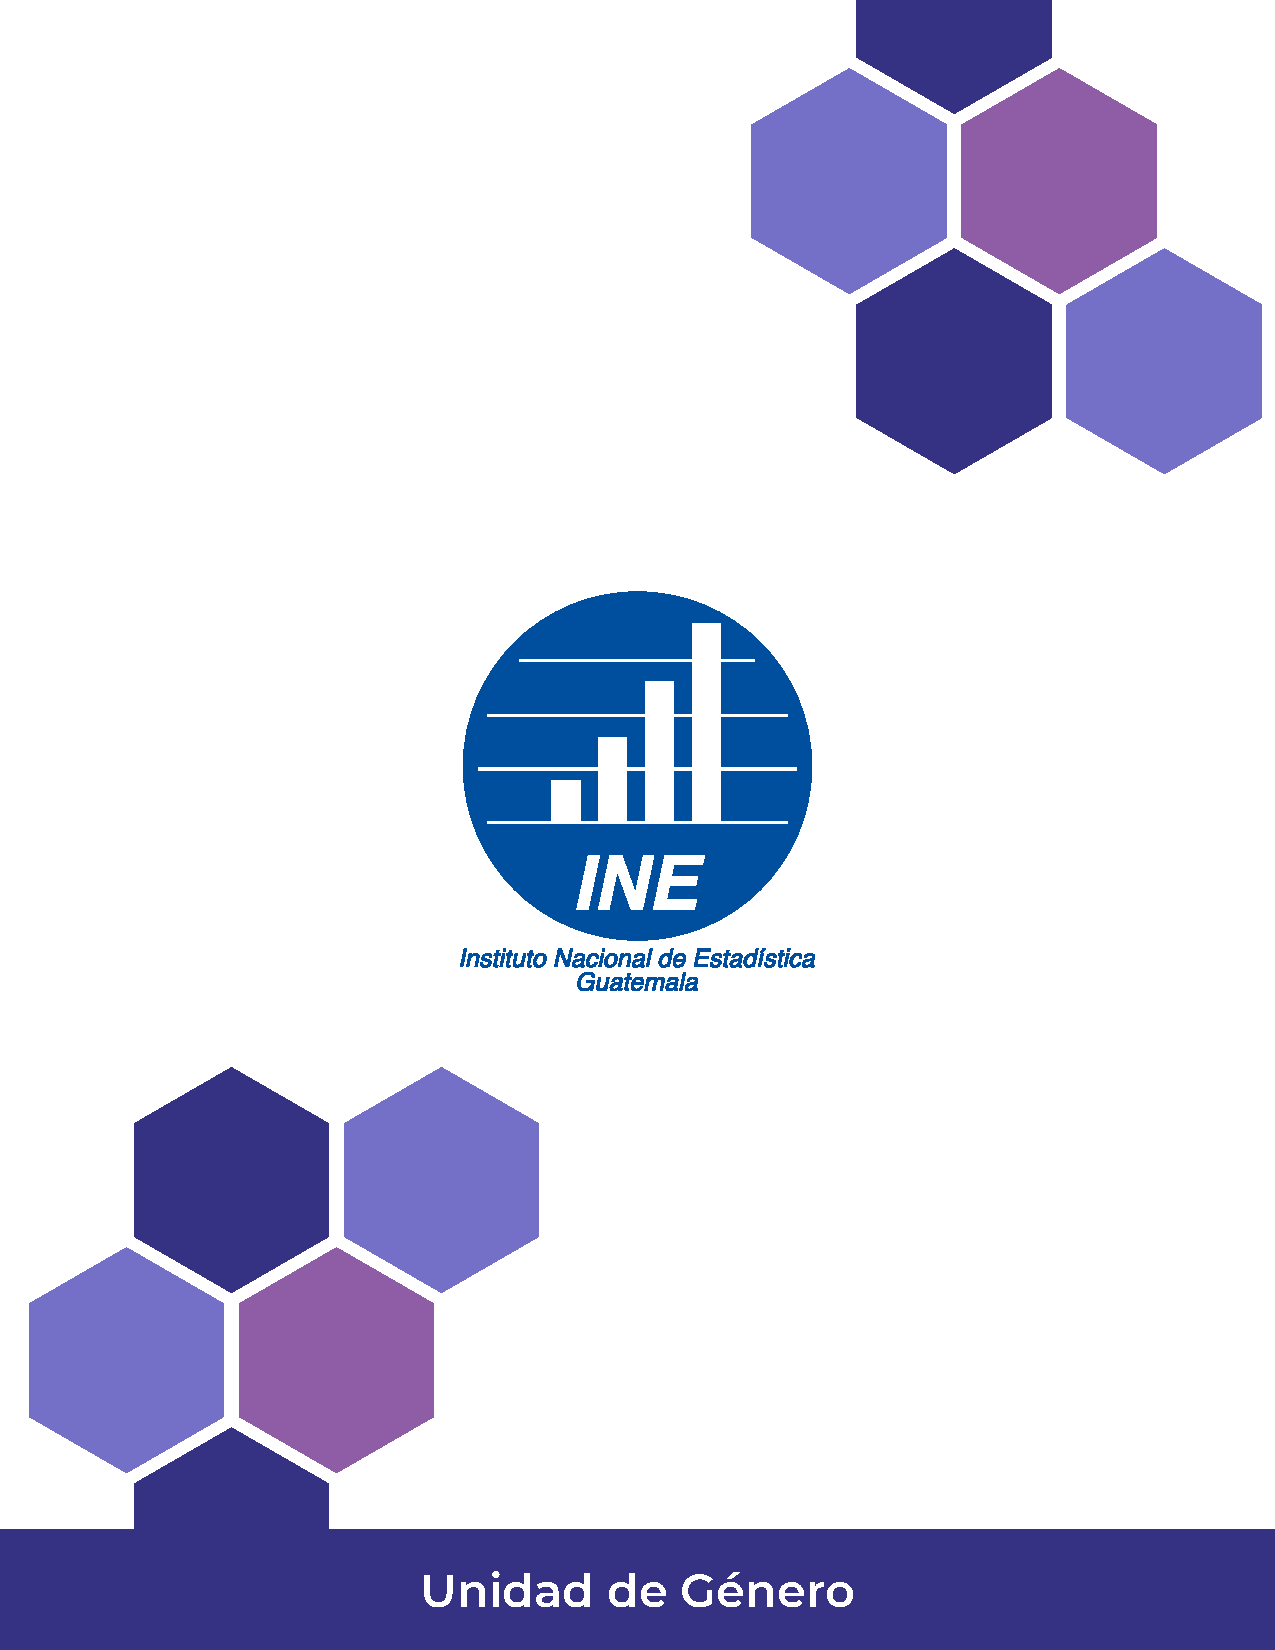
\includepdf{Plantilla/Contraportada_CEEG_2022.pdf}
	
	
\end{document}
	